\documentclass[11pt,a4paper]{article}
\usepackage{polski}
\usepackage[utf8]{inputenc}
\usepackage[titletoc]{appendix}
\usepackage{mathtools}
\usepackage{float}

\usepackage[pdftex]{hyperref}
\usepackage{breakurl}

% by użyć polskich znaków w systemach Linux 
% używamy kodowania "latin2" lub "utf8", dla Windows "cp1250"

% ustawienia marginesow
\usepackage[cm]{fullpage}
\usepackage[top=2.5cm, bottom=2.5cm, left=2.5cm, right=2.5cm]{geometry}

% ustawienia obrazow %
\usepackage{graphicx}
\graphicspath{ {./assets/images/} }
\DeclareGraphicsExtensions{.pdf,.png,.jpg}

% listing kodu
\usepackage{listings}
\usepackage{color}

\definecolor{lightgray}{rgb}{.9,.9,.9}
\definecolor{darkgray}{rgb}{.4,.4,.4}
\definecolor{purple}{rgb}{0.65, 0.12, 0.82}

\lstdefinelanguage{JavaScript}{
  keywords={typeof, new, true, false, catch, function, return, null, catch, switch, var, if, in, while, do, else, case, break},
  keywordstyle=\color{blue}\bfseries,
  ndkeywords={class, export, boolean, throw, implements, import, this},
  ndkeywordstyle=\color{darkgray}\bfseries,
  identifierstyle=\color{black},
  sensitive=false,
  comment=[l]{//},
  morecomment=[s]{/*}{*/},
  commentstyle=\color{purple}\ttfamily,
  stringstyle=\color{red}\ttfamily,
  morestring=[b]',
  morestring=[b]"
}

\lstset{
   language=JavaScript,
   extendedchars=true,
   basicstyle=\small\tt,
   showstringspaces=false,
   showspaces=false,
   numbers=left,
   numberstyle=\footnotesize,
   numbersep=9pt,
   tabsize=4,
   breaklines=true,
   showtabs=false,
   captionpos=b,
   belowskip=1.5em,
   aboveskip=1.5em
}

% document settings
\begin{document}

\begin{titlepage}
    \begin{center}
        
\includegraphics[width=4cm]{assets/images/polsl.jpg}\\[1cm]
        \textsc{\LARGE{Politechnika Śląska}}\\[0.5cm]
        \textsc{\LARGE{Wydział Automatyki, Elektroniki i~Informatyki}}\\[0.5cm]
        \textsc{\LARGE{Kierunek Informatyka}}\\[2.5cm]
        \LARGE{Projekt inżynierski}\\[1cm]
        \begingroup
            \fontsize{14pt}{17pt}\selectfont
            Zdalne sterowanie ze smartfona grą marketingową na interaktywnym bilboardzie LED
        \endgroup
    \end{center}
    \vspace{5cm}
    \begingroup
        \fontsize{14pt}{17pt}\selectfont
        \textbf{Autorzy:} Piotr Pelczar i~Kamil Badyla\\
        \textbf{Kierujący pracą:} dr inż. Przemysław Szmal\\
    \endgroup

    \vspace{3.5cm}
    \begingroup
        \fontsize{12pt}{14pt}\selectfont
        \begin{center}
        Gliwice, styczeń 2013
        \end{center}
    \endgroup
\end{titlepage}

\tableofcontents

% pierwsza sekcja
\section{Tekst}label{sectekst}
LaTeX ułatwia autorowi tekstu zarządzanie 
numerowaniem sekcji, wypunktowaniami oraz odwołaniami 
do tabel, rysunków i~innych elementów. W~łatwy sposób 
możemy się odwołać do wzoru \ref{eqnwzor1}.

% druga sekcja
\section{Matematyka}label{secmatematyka}
Poniższy wzór prezentuje możliwości LaTeX w~zakresie 
składu formuł matematycznych. Wzory są numerowane 
automatycznie, podobnie jak inne elementy o~których 
mowa w~sekcji~\ref{sectekst}.
\begin{equation}
E = mc^2,
\label{eqnwzor1}
\end{equation}
gdzie
\begin{equation}
m = frac{m_0}{sqrt{1-frac{v^2}{c^2}}}.
\end{equation}

\section{Cel}
Celem realizacji naszego projektu jest stworzenie platformy pozwalającej uruchamiać aplikację na wielu rozproszonych monitorach sterowanych przez urządzenia wyposażone w przeglądarkę internetową, oraz bezprzewodową kartę sieciową.  
Istotną zaletą systemu jest całkowita niezależność systemu od marki czy modelu ekranu. Bowiem istniejące rozwiązania na rynku są powiązane z jednym systemem operacyjnym i jedną marką.

\section{Założenia wstępne, określenie wymagań}

\subsection{Wymagania funkcjonalne}



\subsection{Wymagania niefunkcjonalne}



%\section{Motywacja}

TODO:
Dlaczego projekt powstaje? Uzasadnienie.


\newpage
\section{Analiza}
\label{sec:analyse}

\subsection{Klient webowy - pilot uruchomiony na urządzeniu mobilnym}

Kluczowym z punktu widzenia systemu jest poprawnie działający, uniwersalny klient webowy w postaci strony internetowej wyświetlanej w przeglądarce na urządzeniu mobilnym klienta końcowego. Biorąc pod uwagę różnorodność rozdzielczości ekranów, gęstości pikseli (ang. \emph{pixel density}), szybkości wykorzystywanych łącz, wsparcia przeglądarek internetowych na urządzeniach mobilnych dla dyrektyw CSS 3\footnote{CSS (ang. \emph{Cascading Style Sheets}) kaskadowe arkusze stylów, opisujące sposób wyświetlania elementów strony internetowej)}, SVG\footnote{SVG (ang. \emph{Scalable Vector Graphics}) format grafiki wektorowej} rozpoznano szereg problemów oraz zaproponowano rozwiązania.

\subsection{Wykrywanie gestów telefonu komórkowego}
\label{sub:touch-detection}

Pojawienie się na rynku urządzeń dotykowych postawiły przed twórcami interfejsów nowe wyzwania, a projektantom mobilnych przeglądarek internetowych wyzwanie obsługi gestów wykonywanych palcami na ekranie i ich interpretacje na istniejące już, dobrze zakorzenione standardy obsługi zdarzeń myszy.

Przeglądarki internetowe uruchamiane na urządzeniach mobilnych, które przewidują dotykowy sposób komunikacji z interfejsem aplikacji internetowej zazwyczaj odwzorowują dotyk jako zdarzenia myszy (ang. \emph{mouse events}), aby umożliwić interakcję z uruchomioną na ekranie aplikacją. Niestety interpretacja dotyku jako zdarzeń myszy ma pewne ograniczenia użyteczności związane z fizycznym dostępem do treści. Co więcej, w przeglądarce internetowej nie ma możliwości obsługi wielu kursorów jako dotyku kilku palców jednocześnie, ze względu na ograniczenia interfejsu zdarzeń myszy, niezależnie od możliwości urządzenia. Oba te ograniczenia, na poziomie systemowym oraz ze względu na wsteczną zgodność standardów rodzą problemy z obsługą dotyku jako zdarzeń.

\subsubsection{W3C Touch Events specification}

Specyfikacja zdarzeń dotyku (\emph{Touch Events specification}\cite{touch-events-w3c}) opracowana przez W3C\footnote{W3C - World Wide Web Consortium} rozwiązuje powyższe problemy definiując interfejsy umożliwiające aplikacjom bezpośrednią obsługę zdarzeń gestów, z możliwością interpretacji wielu dotyków jednocześnie dla urządzeń zdolnych do ich obsługi. Jej pierwsza wersja (\emph{Proposed Recommendation}) powstała już 5 maja 2011, aż po pięciu poprawkach (przechodząc przez statusy \emph{Working Draft} oraz \emph{Candidate Recommendation}) uzyskała status \emph{W3C Recommendation}.

Definiuje ona interfejs punktu dotyku \emph{Touch} jako obiekt niezmienny (ang. \emph{immutable object}\footnote{Immutable object - Obiekt niezmienny raz utworzony, nie może zmieniać swojego stanu}):

\lstset{language=Octave}
\begin{lstlisting}
interface Touch {
    readonly    attribute long        identifier;
    readonly    attribute EventTarget target;
    readonly    attribute long        screenX;
    readonly    attribute long        screenY;
    readonly    attribute long        clientX;
    readonly    attribute long        clientY;
    readonly    attribute long        pageX;
    readonly    attribute long        pageY;
};
\end{lstlisting}

\begin{description}
  \item[identifier] \hfill \\
  Unikatowy identyfikator punktu dotyku względem pozostałych identyfikatorów już aktywnych\footnote{Można wyobrazić sobie sytuację, gdy nowy punkt dotyku pojawia się, gdy użytkownik dotykał powierzchnię w innych miejscach} punktów dotyku. Każdy punkt dotyku otrzymuje identyfikator w momencie jego zarejestrowania.
  \item[target] \hfill \\
  Obiekt na powierzchni który został wskazany przez punkt dotyku w momencie jego zarejestrowania. Nawet, jeżeli punkt dotyku się przesuwa wskazując inne obiekty, target nie ulega zmianie\footnote{Można wykorzystać ten fakt do zmiany położenia zgodnie ze zmianą pozycji punktu dotyku, np. do przesuwania obiektów}.
  \item[screenX, screenY] \hfill \\
  Współrzędne punktu dotyku względem punktu zerowego ekranu.
  \item[clientX, clientY] \hfill \\
  Współrzędne punktu dotyku względem punktu zerowego powierzchni rzutni na której wyświetlana jest strona internetowa, z wyłączeniem przesunięcia punktu widoczności.
  \item[pageX, pageY] \hfill \\
  Współrzędne punktu dotyku względem punktu zerowego powierzchni rzutni na której wyświetlana jest strona internetowa, z uwzględnieniem przesunięcia punktu widoczności (suma przesunięcia oraz pozycji punktu dotyku na widocznej części rzutni).
\end{description}

Ponadto do obsługi wielu punktów dotyku pojawiających się równolegle zdefiniowano interfejs \lstinline{TouchList} zawierający listę punktów dotyku:

\lstset{language=Octave}
\begin{lstlisting}
interface TouchList {
    readonly    attribute unsigned long length;
    getter Touch? item (unsigned long index);
};
\end{lstlisting}

Aby reagować na zdefiniowane zdarzenia, należy zarejestrować procedurę obsługi zdarzenia. Dostępne są następujące zdarzenia:

\begin{description}
  \item[touchstart] \hfill \\
  Zdarzenie jest wyzwalane, gdy wystąpi pojawienie się nowego punktu dotyku. Jego domyślna implementacja nie jest określona.
  \item[touchend] \hfill \\
  Zdarzenie jest wyzwalane, gdy wystąpi zaniknięcie punktu dotyku. Jego domyślna implementacja zakłada, że wyzwalane jest zdarzenie \lstinline{mousemove}, jeżeli punkt dotyku się kiedykolwiek przemieścił lub wyzwolenie zdarzeń \lstinline{mousedown}, \lstinline{mouseup}, \lstinline{click}, gdy punkt nie zmienił swojego położenia\footnote{Imitacja kliknięcia myszą na urządzeniach dotykowych}.
  \item[touchmove] \hfill \\
  Zdarzenie jest wyzwalane, gdy nastąpi zmiana położenia punktu dotyku.
  \item[touchcancel] \hfill \\
  Zdarzenie jest wyzwalane, gdy punkt dotyku opuszcza dostępną rzutnię lub gdy występuje błąd implementacji. Niezdefiniowane zachowanie.
\end{description}

\subsubsection{Respektowanie standardu Touch Events przez producentów przeglądarek}
\label{subsec:w3c-touch-events-implementations}

Pojawienie się propozycji standardu nie gwarantuje, że producenci popularnych przeglądarek internetowych zaimplementują daną funkcjonalność wg podanej specyfikacji, bądź czy obsługa w ogóle występuje. W chwili obecnej biorąc pod uwagę przeglądarki internetowe dla urządzeń mobilnych, standard jest wspierany przez\cite{caniuse-touch-events}:

\begin{enumerate}
  \item \textbf{iOS Safari}\cite{browser-ios-safari} \footnote{\cite{browser-ios-safari} Rozdział \em{Handling events}, \url{https://developer.apple.com/library/ios/documentation/AppleApplications/Reference/SafariWebContent/HandlingEvents/HandlingEvents.html}}, natywna przeglądarka systemu iOS firmy Apple;
  \item \textbf{Android Browser}, natywna przeglądarka systemu Android;
  \item \textbf{Blackberry Browser},
  \item \textbf{Firefox} - określa własny, bardzo podobny standard, dzięki któremu można osiągnąć te same efekty\cite{browser-firefox} \footnote{\cite{browser-firefox} Rozdział \em{Touch events}, \url{https://developer.mozilla.org/en-US/docs/Web/Guide/Events/Touch_events}}.
\end{enumerate}

Przeglądarki nie wspierające standardu:

\begin{enumerate}
  \item \textbf{Opera Mini},
  \item \textbf{IE Mobile}, własny standard, niekompatybilny\cite{browser-ie} \footnote{\cite{browser-ie} Rozdział \em{Pointer and gesture events}, \url{http://msdn.microsoft.com/en-us/library/ie/hh673557(v=vs.85).aspx}}.
\end{enumerate}

\subsection{Pamięć podręczna Web Storage}
\label{subsub:webstorage}

Klient webowy uruchomiony na urządzeniu mobilnym zawiera pliki z kodem JavaScript, które są pobierane do przeglądarki internetowej celem ich interpretacji i późniejszego wykonania. Ze względu na specyfikę sieci 3G: mniejsza przepustowość (ang. \emph{bandwidth}), koszt transferu (ponoszony przez użytkownika końcowego), większe opóźnienia (ang. \emph{latency}) niezbędnym jest zapamiętywanie lokalnie pobranych plików, celem ich ponownego otwarcia z lokalnej przestrzeni dyskowej urządzenia, bez konieczności dostępu do nich przez sieć.

Przeglądarki internetowe na urządzeniach mobilnych wspierają pamięć tymczasową \emph{cache} protokołu HTTP opisaną w dokumencie RFC-2616 \emph{Hypertext Transfer Protocol - HTTP/1.1}\cite{http-rfc} \footnote{Rozdział 13, \emph{Caching in HTTP}}. Można by było zadać pytanie, czy pamięć jest zachowywana po zamknięciu przeglądarki na urządzeniu mobilnym jako aplikacji, przy blokowaniu i wyłączaniu telefonu. Wykonane testy dowodzą, że przeglądarki internetowe na urządzeniach mobilnych wykazują poprawne zachowanie\cite{http-cache-mobile-benchmark}.

Można by było zaprzestać na serwowaniu plików JavaScript z nagłówkiem \lstinline{Cache-Control} oraz \lstinline{Expires} na bardzo odległy czas, przykładowo:

\lstset{language=Octave}
\begin{lstlisting}
Cache-Control: max-age=315360000, must-revalidate
Expires: Mon, 30 Oct 2023 14:19:41 GMT
\end{lstlisting}

\subsubsection{Wydajność Web Storage}
\label{subsub:webstorage-performance}

Zaproponowany standard W3C \emph{Web Storage}\cite{webstorage}\footnote{W3C Recommendation, {\em Web Storage}, \url{http://www.w3.org/TR/webstorage/}}, który również zapewnia przechowywanie danych lokalnie, dał początek testom związanych z szybkością ładowania plików z obu pamięci podręcznych. Local Storage to pamięć asocjacyjna klucz-wartość (ang. \emph{key-value storage}), gdzie zarówno klucz, jak i wartość są ciągiem znaków. Wartości JavaScript nie będące ciągiem znaków są na niego rzutowane.

Co prawda, w swoim zamierzeniu Web Storage nie miał na celu przechowywanie plików wchodzących w skład strony internetowej, ale posiada interfejs, który umożliwia wykorzystanie go właśnie w ten sposób. Wykonane testy wykazały, że ładowanie danych z Web Storage (dokładniej \emph{Local Storage}) jest nawet do 5 razy szybsze, niż w przypadku ładowania danych z pamięci podręcznej przeglądarki (\emph{Native cache})\cite{http-cache-mobile-benchmark}\footnote{Testy dotyczące przeglądarek internetowych na urządzeniach mobilnych opublikowanych 13 maja 2013 przez Petera McLachlana}:

\begin{figure}[h!]
  \caption[Porównanie czasu ładowania danych z cache przeglądarki oraz Web Storage]{Czerwoną kreską oznaczono średnią.}
  \centering
    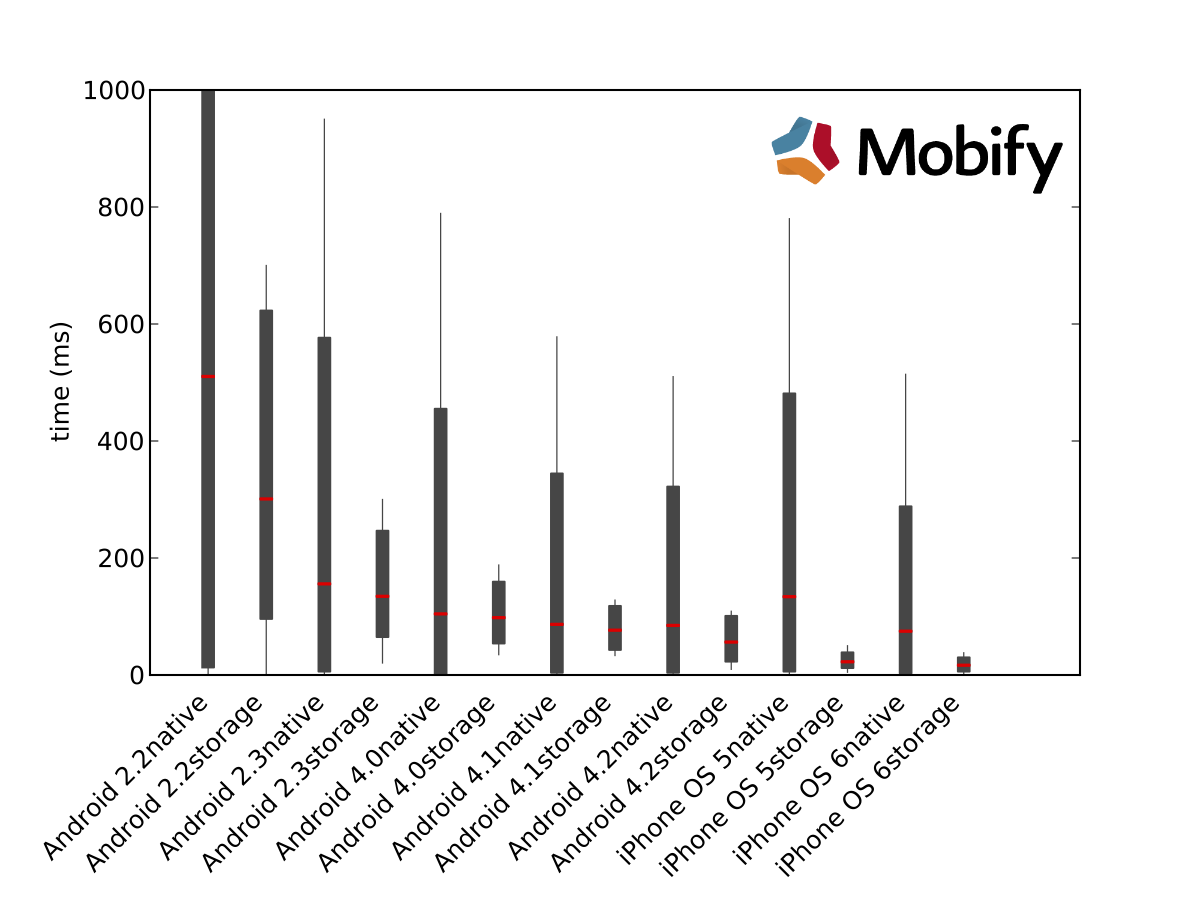
\includegraphics[width=\textwidth]{localstorage-benchmark}
\end{figure}

\begin{center}
    \begin{tabular}{ | l | p{2.5cm} | p{2.5cm} | p{2.5cm} | p{2.5cm} |}
    \hline
	Smartphone OS & localStorage \newline śr. (ms) & native browser \newline śr. (ms) & localstorage \newline odch. st. & native browser \newline odch. st. \\ \hline
	Android 2.2 & 299.94 & 509.32 & 164.76 & 537.95 \\ \hline
	Android 2.3 & 133.50 & 154.76 & 57.65 & 215.13 \\ \hline
	Android 4.0 & 97.05 & 103.44 & 31.80 & 179.36 \\ \hline
	Android 4.1 & 75.60 & 85.57 & 21.60 & 132.03 \\ \hline
	Android 4.2 & 55.28 & 83.76 & 23.28 & 121.51 \\ \hline
	iPhone iOS5 & 21.61 & 132.90 & 8.64 & 177.69 \\ \hline
	iPhone iOS6 & 15.71 & 73.86 & 7.27 & 109.32 \\ \hline
    \hline
    \end{tabular}
\end{center}

W przypadku Local Storage zarówno średni czas ładowania, jak i wariancja i odchylenie standardowe jest znacznie mniejsze.

Dokument standardu W3C\cite{webstorage} definiuje sposób dostępu do danych z pamięci lokalnej przeglądarki. Propozycja wynikła z faktu, iż dane zachowane lokalnie w przeglądarce internetowej przed jego pojawieniem się, implementowane za pomocą mechanizmu ciasteczek (ang. \emph{Cookies}) brały udział w transmisji w protokole HTTP jako dane nagłówkowe wychodzące od strony klienta do serwera, co nie było pożądane ze względu na dodatkowy narzut transmisji. Ponadto serwer jest świadom istnienia danych lokalnych i jest w stanie je odebrać (nagłówek HTTP \lstinline{Cookie: } podczas wysyłania żądania do serwera) oraz, co gorsza modyfikować (nagłówek HTTP \lstinline{Set-Cookie: } podczas wysyłania odpowiedzi od serwera).

Przykładowe żądanie HTTP z ciasteczkiem:
\lstset{language=Octave}
\begin{lstlisting}
GET / HTTP/1.1
Host: www.example.org
Cookie: name=value; name2=value2
Accept: */*
\end{lstlisting}

Przykładowa odpowiedź HTTP z modyfikacją ciasteczka:
\lstset{language=Octave}
\begin{lstlisting}
HTTP/1.0 200 OK
Content-type: text/html
Set-Cookie: name=value
Set-Cookie: name2=MODIFIED_VALIE; Expires=Wed, 09 Jun 2021 10:18:14 GMT

(content of page)
\end{lstlisting}

Standard definiuje pamięć jako interfejs \emph{Storage}, na którym można dokonywać operacji odczytu, zapisu, usunięcia.

\lstset{language=Octave}
\begin{lstlisting}
interface Storage {
  readonly attribute unsigned long length;
  DOMString? key(unsigned long index);
  getter DOMString? getItem(DOMString key);
  setter creator void setItem(DOMString key, DOMString value);
  deleter void removeItem(DOMString key);
  void clear();
};
\end{lstlisting}

Istnieją dwa rodzaje pamięci:

\begin{description}
  \item[Local Storage] \hfill \\
  Przypisany dla danego źródła \emph{Origin}\footnote{Origin to zestaw wartości w postaci: \emph{protocol://domain:port}, gdzie \emph{protocol} to skrótowa nazwa protokołu (np http, https), \emph{domain} to nazwa hosta oraz \emph{port} to numer portu, pod którym jest uruchomiona dana usługa} a trybucie \emph{document} pamięć typu \emph{Storage}. Oznacza to, że każda strona internetowa otwarta w przeglądarce posiada swoją niezależną pamięć podręczną, niedostępną dla stron internetowych uruchomionych z innego adresu (protokół, nazwa hosta, numer portu). \emph{Same Origin Policy} zapewnia, że jedna pamięć może być dzielona tylko i wyłącznie między dokumentami otwartymi przez przeglądarkę dla tej samej nazwy hosta, uruchomiona na wybranym, określonym porcie oraz przekazywana jednym określonym protokołem (np. http, czy https). Dla każdej różnej kombinacji tworzona jest oddzielna pamięć, a dokumenty nie mają dostępu do swoich pamięci na wzajem. Pamięć \emph{Local Storage} ma nieograniczony czas życia, nie ulega zdezaktualizowaniu, dopóki nie zabraknie limitowanego miejsca\footnote{Ilość miejsca jest różna dla przeglądarek} lub użytkownik nie wyczyści danych przeglądarki ręcznie.
  \item[Session Storage] \hfill \\
  Ma te same właściwości, jak \emph{Local Storage} za wyjętkiem tej, że pamięć jest czyszczona po zamknięciu sesji, tj. po zamknięciu wszystkich okien dla danego \emph{Origin}.
\end{description}

\subsubsection{Respektowanie standardu Web Storage przez producentów przeglądarek}

Zaraz po wprowadzeniu propozycji Web Storage, producenci przeglądarek internetowych szybko wprowadzili nową, spójną funkcjonalność. Tendencja utrzymuje się do dziś. Przeglądarki mobilne wspierające standard\cite{caniuse-webstorage}:

\begin{enumerate}
  \item iOS Safari,
  \item Android Browser,
  \item Blackberry Browser,
  \item Opera Mobile,
  \item Chrome for Android,
  \item Firefox for Android,
  \item IE Mobile.
\end{enumerate}

Przeglądarki nie wspierające standardu:

\begin{enumerate}
  \item Opera Mini
\end{enumerate}

\subsection{Projektowanie stron internetowych zgodnie z Responsive Web Design}
\label{subsubsec:rwd}

\emph{Responsive Web Design} (RWD) to sposób projektowania stron internetowych przyjaznych do przeglądania oraz obsługiwania na szerokiej gamie rozdzielczości ekranów (począwszy na urządzeniach mobilnych, po netbooki, komputery jak i monitory z dużą rozdzielczością)\cite{rwd}; rozumianej jako brak konieczności skalowania, przewijania pasków przez użytkownika. Zaprojektowane w ten sposób strony internetowe potrafią zmieniać swój układ, rozmiar grafik, czcionek w zależności od wymiarów widocznej powierzchni ekranu (ang. \emph{viewport}).

\subsubsection{Viewport}

Viewport to widoczna część strony internetowej w oknie przeglądarki. W ramach tej części wykonywana jest projekcja rzutni, na której generowana jest strona internetowa w graficznej postaci. Jeżeli rozmiar rzutni strony internetowej jest większy niż viewport, użytkownik nawiguje się po jej zawartości przeciągając pasek przesówania (horyzontalny i/lub wertykalny).

Na rysunkach poniżej prezentowany jest przykładowy viewport w kontekście wyświetlenia strony internetowej:

\begin{figure}[h!]
  \caption[Apple default viewport w Safari iOS]{Domyślny viewport iOS Safari na urządzeniu firmy Apple.}
  \centering
    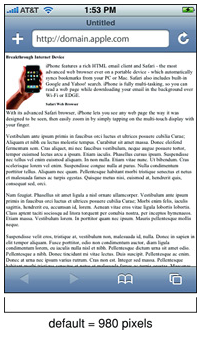
\includegraphics[scale=0.75]{viewport-default.png} \\
    Domyślnie w przeglądarce iOS Safari viewport wynosi 980 pikseli szerokości, mimo, iż ekran optymalnie wyświetla 320 pikseli. Aby przedstawić całą stronę internetową szerokość jest dobierana automatycznie.
\end{figure}

Podczas projektowania interfejsu strony internetowej wyświetlanej na stronie internetowej istotne jest okreslenie viewportu, aby uniknąć nieoczekiwanemu przyjęciu domyślnych wartości, bowiem strategie ich okreslania są różne. Niektóre przeglądarki dopasowują szerokość viewportu do najszerszego elementu strony internetowej, co powoduje, że tekst i elementy interaktywne mogą być niewidoczne. Aby przyjąć szerokość viewportu zgodne z szerokością przeglądarki internetowej na urządzeniu, należy zdefiniować wartość jako \lstinline{device-width}, wówczas szerokość strony zostanie przycięta, a w przypadku projektowania interfejsu zgodnie z zasadą Responsive Web Design (opisanum w podsekcji \ref{subsubsec:rwd}), istnieje możliwość określenia dedykowanych arkuszy styli definiujących wygląd strony w zależności od szerokości viewportu (który nie może być zmieniany na urządzeniu mobilnym, a w przypadku przeglądarki uruchomionej na komputerze - tak, poprzez zmianę rozmiaru okna).

\begin{figure}[h!]
  \caption[Apple fixed viewport w Safari iOS]{Ustawiony viewport iOS Safari na urządzeniu firmy Apple}
  \centering
    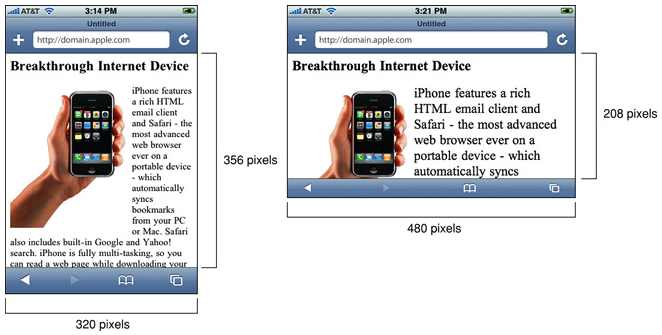
\includegraphics[scale=0.75]{viewport-adjusted.png} \\
    Viewport można regulować ustawiając stałe wartości, np 320px lub \lstinline{device-width} jako szerokość okna przeglądarki.
\end{figure}

\lstset{language=HTML}
\begin{lstlisting}
<meta name="viewport" content="width=device-width" />
\end{lstlisting}

\subsubsection{Cascading Style Sheet - Media Queries}

Znane są rozszerzenia kaskadowych arkuszy styli (ang. \emph{Cascading Style Sheet}, w skrócie \emph{CSS}) z wersji 2.1\cite{css21}, gdzie za pomocą atrybutu \emph{@media} istnieje możliwość zdefiniowania, jakiego typu urządzenia dotyczy wybrany arkusz styli\footnote{\cite{css21}, Rozdział \emph{Media types}}, tzw \emph{Media Queries}, np:

\begin{description}
  \item[all] \hfill \\
  Wszystkie urzadzenia
  \item[print] \hfill \\
  Dla urządzeń drukujących lub stron na ekranie wyświetlanych w trybie podglądu do wydruku.
  \item[handheld] \hfill \\
  Dla urządzeń kieszonkowych o zmniejszonej rozdzielczości ekranu.
  \item[projection] \hfill \\
  Dla urządzeń, które wyświetlają stronę w trybie prezentacyjnym, np projektorów.
  \item[tty] \hfill \\
  Dla urządzeń o ściśle określonym obszarze na wyświetlanie znaków, np. terminale, urządzenia przenośne z okraniczonym tekstowym wyświetlaczem.
\end{description}

Sposob załączania arkusza w zależności od jego przeznaczenia jest następujący dla dokumentu HTML:

\lstset{language=HTML}
\begin{lstlisting}
<link rel="stylesheet" type="text/css" href="layout.css"
  media="screen" />
<link rel="stylesheet" type="text/css" href="print.css"
  media="print" />
\end{lstlisting}

Lub bezpośrednio w arkuszu stylów:

\lstset{language=Octave}
\begin{lstlisting}
@media print {
  body { font-size: 10pt }
}
@media screen {
  body { font-size: 13px }
}
@media screen, print {
  body { line-height: 1.2 }
}
\end{lstlisting}

Nie jest to jednak wystarczające w kontekście dostosowania strony internetowej do rozmiarów i rozdzielczości okna przeglądarki. W CSS w wersji 3.1 wprowadzono możliwość załączania styli w zależności od rozdzielczości dostępnej powierzchni (\emph{viewport}) za pomocą rozszerzonego o tę możliwość \emph{Media Queries}\cite{css3}\footnote{\cite{css3} Rozdział \emph{Media Queries}, http://www.w3.org/TR/css3-mediaqueries/}.

Pojawiła się między innymi wartość atrybutu \lstinline{@media}: \lstinline{device-width} oraz \lstinline{device-height} z przedrostkami \lstinline{min-} i \lstinline{max-}, co w pełni wyczerpuje potrzeby projektowania stron internetowych zgodnie z RWD.

Przykładowy kod ładujący arkusz styli dla urządzeń o maksymalnej szerokości 480px:

\lstset{language=Octave}
\begin{lstlisting}
<link rel="stylesheet" type="text/css"
  media="screen and (max-device-width: 480px)"
  href="landscape.css" />
\end{lstlisting}


\subsection{Serwer}

Klient webowy uruchamiany w przeglądarce internetowej na urządzeniu mobilnym użytkownika końcowego łączy się z serwerem przez sieć\footnote{Diagram komponentów w dodatku \ref{app:network_diagram_app}}, odpowiadającym za poprawne działanie systemu. Korzystając z nowych możliwości przeglądarek internetwoych zaimplementowano dwustronną komunikację (ang. \emph{full duplex communication}) przy użyciu mechanizmu \emph{Web Sockets}\cite{websockets-rfc} opisaną w podsekcji \ref{subsub:websockets}. Dla urządzeń nie obsługujących standardu Web Sockets, przy użyciu biblioteki \emph{Socket.io} (opisanej w podsekcji \ref{subsub:socketio}) dostępne są inne mechanizmy (przegląd w podsekcji \ref{sub:communication-methods}) dwustronnej komunikacji nie wykazujące tak szybkiego działania.

\subsection{Komunikacja między klientem webowym, a serwerem}

W obu aplikacjach, zarówno w grze PONG, jak i w pilocie sterującym zdalnym monitorem, komunikacja między rozproszonym systemem jest oparta o asynchroniczną wymianę komunikatów (ang. \emph{Asynchronous Message-oriented middleware - MOM})\cite{message-oriented-middleware}.

Przeprowadzano dywagację na temat skalowania stworzonego systemu opisaną w podsekcji \ref{subsub:scalability}. W obliczu skalowalności klienci łączą się do centralnego serwera, który rozdysponuje ruch sieciowy pomiędzy dostępne serwery (ang. \emph{nodes}) obsługujące żądania. W kontekście rozproszenia systemu, architektura MOM polega na asynchronicznym modelu wymiany komunikatów, w przeciwieństwie do modelu żądanie-odpowiedź (\emph{request-response model}). W asynchronicznych systemach kolejki komunikatów pełnią rolę tymczasowego bufora, kiedy odbiorca wiadomości jest zajęty lub niepodłączony do sieci. W dodatku istnieje możliwość stworzenia kolejek trwałych (ang. \emph{persistent queues}), w których wiadomości są zapisywane w pamięci trwałej (np. na dysku) zachowania ich kopii, dzięki czemu nadawca i odbiorca wiadomości nie musi być dostępny w sieci w tym samym czasie - mechanizm ten nazywany jest asynchroniczną dostawa (ang. \emph{asynchronous delivery}). Oznacza to, że gdy odbiorca wiadomości jest niedostępny, wysyłający wiadomości może pracować, a wiadomości zostaną odłożone w kolejce celem późniejszej dostawy, kiedy odbiorca będzie dostępny.

\begin{figure}[H]
  \centering
    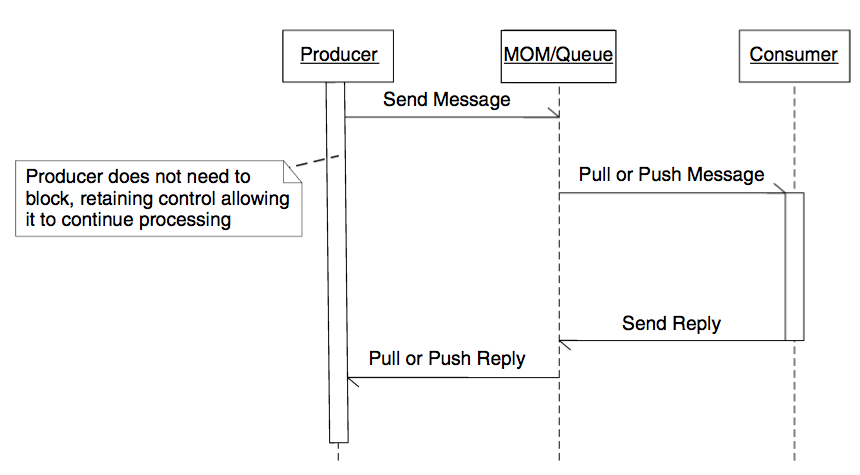
\includegraphics[width=\linewidth]{mom-flow.png}
  \caption[Model asynchronicznej interakcji w systemach opartych o wymianę komunikatów]{Model asynchronicznej interakcji w systemach opartych o wymianę komunikatów}
    Diagram UML przepływu przedstawiający model producenta i konsumenta wiadomości połączonego przez system kolejek (źródło: Edward Curry, \emph{Message-Oriented Middleware}\cite{message-oriented-middleware})
\end{figure}

\begin{figure}[H]
  \centering
    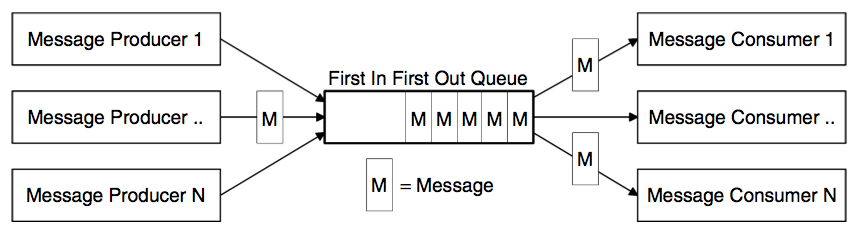
\includegraphics[width=\linewidth]{mom-queue.png}
  \caption[Schemat działania kolejki w systemach opartych o wymianę komunikatów]{Schemat działania kolejki w systemach opartych o wymianę komunikatów}
    Diagram przedstawiający model producenta i konsumenta wiadomości połączonego przez system kolejek FIFO, (źródło: Edward Curry, \emph{Message-Oriented Middleware}\cite{message-oriented-middleware})
\end{figure}

\subsection{Komunikacja HTTP - model Comet}
\label{sub:communication-methods}

Protokół HTTP\footnote{Hypertext Transfer Protocol} przewiduje komunikację inicjowaną przez klienta do serwera\cite{http-rfc}. Klient wysyła żądanie (ang. \emph{request}) złożone z nagłówków (ang. \emph{headers}) oraz treści (ang. \emph{body} lub \emph{content}), natomiast serwer zwraca odpowiedź również w postaci nagłówków oraz treści. Każde żądanie jest bezstanowe, swego rodzaju transakcją, to znaczy, że nie zależy od poprzedniego, ani kolejnego. Aby zapewnić transakcyjność stosuje się mechanizmy podtrzymania sesji użytkownika za pomocą przesyłania w nagłówkach ciasteczek zawierający unikatowy identyfikator sesji znany zarówno po stronie klienta, jak i serwera - tym sposobem serwer jest w stanie zidentyfikować następujące po sobie bezstanowe żądania. Istotnym minusem w kontekście prowadzenia komunikacji w protokole HTTP jest to, że serwer nie może zainicjować wysłania danych do przeglądarki, bowiem połączenie jest zamykane zaraz po odesłaniu odpowiedzi. Komunikacja jest jednostronna (ang. \emph{half-duplex communication}).

Przykładowe zapytanie:
\lstset{language=Octave}
\begin{lstlisting}
GET /path/file.html HTTP/1.1\r\n
Host: www.host1.com:80\r\n
\r\n
\end{lstlisting}

Przykładowa odpowiedź:
\lstset{language=Octave}
\begin{lstlisting}
HTTP/1.1 200 OK\r\n
Date: Fri, 31 Dec 1999 23:59:59 GMT\r\n
Content-Type: text/plain\r\n
Transfer-Encoding: chunked\r\n
\r\n \#\# oznacza pusta linie
TUTAJ TRESC
\end{lstlisting}

Aby zapewnić komunikację dwustronną (ang. \emph{full-duplex communication}) (tj. aby serwer mógł wysyłać wiadomości do przeglądarki internetowej w trybie \emph{server push}) stosuje się wiele zabiegów, znanych ogólnie pod pojęciem \emph{Comet} (modelu komunikacji polegającym na wykorzystaniu zawieszonych połączeń HTTP, ang. \emph{long-held HTTP requests}), których przegląd jest zamieszczony poniżej. Inne znane nazwy tożsame z Comet: \emph{Ajax Push},\footnote{ICEfaces.org [Data dostępu: 27 grudnia 2013]} \emph{Reverse Ajax}\footnote{Crane, Dave; McCarthy, Phil (Lipiec 2008). \emph{Comet and Reverse Ajax: The Next Generation Ajax 2.0}. Apress. ISBN 1-59059-998-5}, \emph{Two-way-web}, \emph{HTTP Streaming}, \footnote{Mahemoff, Michael (Czerwiec 2006). \emph{Web Remoting}. Ajax Design Patterns. O'Reilly Media. s. 19; 85. ISBN 0-596-10180-5}, oraz \emph{HTTP server push}\footnote{Double, Chris (2005-11-05). \emph{"More on Ajax and server push". Different ways of doing server push.}}.

\subsubsection{Komunikacja HTTP persistent connection}
\label{subsub:http-persistent-connection}

Protokół HTTP w wersji 1.0 umożliwia tworzenie stałych połączeń (ang. \emph{persistent connection}) przez przesłanie nagłówka Connection: Keep-Alive, serwer w ramach odpowiedzi odsyła ten sam nagłówek, a od wersji protokołu 1.1 Keep-Alive jest uznawane za domyślne i nie jest konieczne wysłanie nagłówka. Otwarte połączenie przez przeglądarkę internetową nie zamyka go tuż po otrzymaniu odpowiedzi od serwera, a podtrzymuje je mogąc wysłać w ramach niego kilka żądań. Optymalizacja ma na celu zmniejszenie czasu wykonywania żądań o czas otwarcia połączenia po stronie przeglądarki internetowej oraz serwera. Korzyści jest znacznie więcej:

\begin{itemize}
	\item mniejsze zużycie procesora i pamięci operacyjnej,
	\item możliwość wykonania kilku żądań i odpowiedzi jedno po drugim (ang. \emph{pipelining}),
	\item zmniejszenie ruchu sieci (mniej połączeń TCP),
	\item zmniejszone opóźnienie (ang. \emph{latency}) związane z nawiązaniem połączenia z odległym hostem,
	\item w przypadku żądań HTTPS\footnote{Secured HTTP, połączenie podpisane certyfikatem SSL} zmniejsza się liczba obiegów sieci (ang. \emph{network round-trips}) celem wymiany kluczy publicznych oraz certyfikatu.
\end{itemize}

\begin{figure}[H]
  \centering
    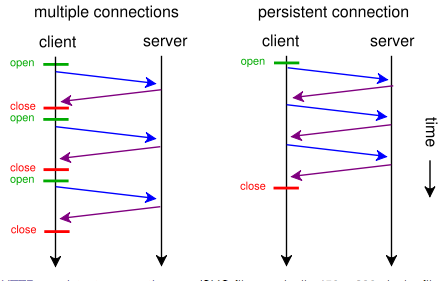
\includegraphics[scale=0.65]{http-persistent-connection.png}
  \caption[HTTP Persistent Connection]{HTTP Persistent Connection}
    Rysunek przedstawia wysyłanie kolejnych żądań HTTP w ramach osobnych połączeń (domyślnie HTTP 1.0, po lewej stronie) oraz w ramach jednego połączenia (persistent connection, po prawej). Źródło: \url{http://en.wikipedia.org/wiki/HTTP_persistent_connection}.
\end{figure}

\subsubsection{HTTP Server Push, Pushlet, JSONP Pooling oraz Script Tag \mbox{long pooling}, Hidden IFRAME}

Powstanie \emph{persistent connections} (opisanego w podsekcji \ref{subsub:http-persistent-connection}) umożliwiło wypracowanie mechanizmów umożliwiających komunikację ze strony od serwera do klienta w trybie push:

\begin{description}
  \item[HTTP Server Push] \hfill \\
  Mechanizm polega na tym, że klient inicjuje żądanie, serwer natomiast podtrzymuje je w trybie zawieszonym (nie odsyła odpowiedzi, połączenie pozostaje otwarte), a gdy wystąpi zdarzenie, może zostać ono wysłane do klienta w trybie natychmiastowym. Jeżeli zachodzi zdarzenie, a klient nie jest podłączony, może zostać dodane do kolejki do wysłania przy następnym żądaniu klienta. Po otrzymaniu odpowiedzi i zerwaniu połączenia klient inicjuje nowe żądanie, powtarzając cały proces w pętli. Zwalnia to z konieczności periodycznego sprawdzania, czy zaszły jakieś zdarzenia na serwerze poprzez odpytywania serwera (ang. \emph{pooling}).

  \begin{figure}[H]
    \centering
      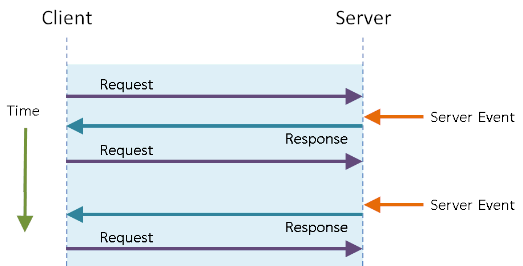
\includegraphics[scale=0.75]{http-server-push.png}
    \caption[Zasada działania HTTP Server Push]{Zasada działania HTTP Server Push}
  \end{figure}

  \begin{figure}[H]
    \centering
      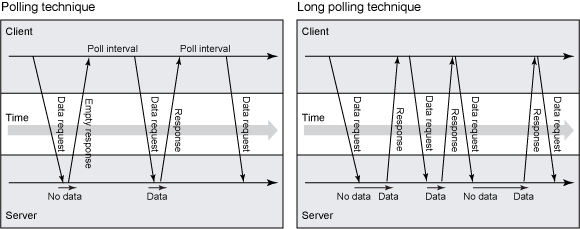
\includegraphics[scale=0.65]{http-pooling-vs-longpooling.jpg}
    \caption[Porównanie HTTP Pooling oraz HTTP Long Pooling]{Porównanie HTTP Pooling oraz HTTP Long Pooling}
  \end{figure}

  \item[Pushlet] \hfill \\
  Podejście polegające na podtrzymaniu zainicjowanego połączenia przez klienta w trybie zawieszonym w stanie ciągłego ładowania odpowiedzi (serwer nigdy nie zamyka połączenia). Umożliwia to ciągłe dostarczanie treści do odpowiedzi, która jest interpretowana przez przeglądarkę, np w postaci kodu JavaScript, osiągając w ten sposób możliwość wysyłania odpowiedzi z serwera do klienta. W ten sposób po stronie klienta nie jest konieczne uruchomienie appletu Java lub kodu Flash, które dostarczają opcję otwarcia połączenia, natomiast wymagają zezwolenia od użytkownika.

  \item[XHR Pooling] \hfill \\
  Możliwe jest posłużenie się obiektem \lstinline{XMLHttpRequest} (\emph{XHR})\cite{xhr-rfc} wykorzystywanym w aplikacjach AJAX (ang. \emph{Asynchronous JavaScript and XML}), który umożliwia asynchroniczne odbieranie framgmentów treści strony bez konieczności odświeżenia całej jej zawartości (ponowienia żądania i odpowiedzi). Dane mogą być odbierane w dowolnym formacie, co umożliwia wykorzystanie mechanizmu Comet.\\

  W 1995 roku przeglądarka Netscape Navigator wprowadziła mechanizm który umożliwił serwerowi odświeżanie zawartości obrazka lub kodu HTML za pomocą wysyłania odpowiedzi wieloczęściowej (ang. \emph{multipart response}) oznaczając ją nagłówkiem

\lstinline{Content-type: multipart/x-mixed-replace}\cite{xhr-rfc}

  Po stronie serwera, każde zdarzenie, które ma być wysłane do klienta, jest kolejną częścią odpowiedzi HTTP, odbierane po stronie klienta i interpretowane w wywoływanej funkcji wskazanej jako \lstinline{onreadystatechange callback} wykonywanej za każdym razem, gdy pojawią się nowe dane. Umożliwia to dosyłanie dowolnych porcji danych.

  \item[Hidden IFRAME] \hfill \\
  Technika znana również pod nazwą \emph{forever frame}, polegająca na umieszczeniu w kodzie strony www ukrytej ramki (umożliwiającej wstawienie dokumentu HTML pochodzącego z innej strony internetowej) wykorzystującej mechanizm Pushlet. Gdy wystąpi zdarzenie na serwerze, może ono zostać wysłane jako treść odpowiedzi w postaci tagu HTML
  \lstinline{<script>}
  wypełnionego treścią wykonywalnego kodu JavaScript, który jest natychmiastowo interpretowany przez przeglądarkę. Dokument HTML przyrasta o nowe tagi \lstinline{<script>}. Podstawową zaletą tego rozwiązania jest to, że jest obsługiwane przez każdą przeglądarkę.

  \item[Script Tag long pooling] \hfill \\
  Wszystkie wyżej wymienione sposoby komunikacji w trybie push od strony serwera wykorzystujące protokół HTTP nie są zdolne do wykonania żądania inicjującego przez klienta pod adres wskazujący na inną domenę, niż otwarta przez użytkownika ze względu na \emph{Same Origin Policy}, bowiem nie można wykonywać połączeń XHR poza domenę\footnote{SLDs - second-level domains} oraz przechwytywać zdarzeń JavaScript z ramki IFRAME z innej domeny. Istnieje sposób na odebranie danych spoza domeny za pomocą załadowania kodu JavaScript przy użyciu tagu \lstinline{<script>}, który może wskazywać dowolny adres URL wykorzystując technikę Pushlet oraz reagować na każdorazowe kolejne doładowanie danych w postaci fragmentu kodu JavaScript, który jest natychmiastowo wykonywany po stronie przeglądarki użytkownika.
  
  \item[JSONP Pooling] \hfill \\
  Oparta na technice \emph{Script Tag long pooling} polegająca na doładowywaniu kodu JavaScript zawierającego dane w postaci JSON\footnote{JSON - JavaScript Object Notation} przekazywane jako argument nazwanej wcześniej przez programistę funkcji\footnote{do adresu URL przekazuje się argument, którego wartością jest nazwa funkcji} w postaci obiektu JavaScript.
  
  Przykład wywołania JSONP Pooling ze wskazaniem funkcji \lstinline{parseResponse()} w atrybucie \emph{functionName}:
\lstset{language=HTML}
\begin{lstlisting}
  <script type="application/javascript"
     src="http://example.com/?functionName=parseResponse">
  </script>
\end{lstlisting}
  
  Jako argument zapytania zostanie wysłana nazwa funkcji, którą serwer umieszcza w odpowiedzi. Jako treść kodu JavaScript wywołuje wskazaną funkcję. Przykładowa odpowiedź serwera:

\lstset{language=JavaScript}
\begin{lstlisting}
   parseResponse({"Name": "Foo", "Id": 1234, "Rank": 7});
\end{lstlisting}

\end{description}

\subsubsection{Metody oparte o wykorzystanie Flash i Java Applets}

Wykorzystując możliwości osadzanych niewidocznych (lub małych, 1x1 pikseli\footnote{one-pixel element}) elementów Flash oraz appletów Java możliwe jest otwarcie połączenie TCP bezpośrednio z tych elementów, a komunikacja z przeglądarką internetową odbywa się za pomocą wywoływania funkcji JavaScript z przekazywanymi danymi. Niestety, Flash oraz applety Java nie są obsługiwane przez większość przeglądarek na urządzeniach mobilnych, a każda interakcja często jest poprzedzona zgodą klienta.

\subsubsection{Web Sockets}
\label{subsub:websockets}

Opisane w sekcji \ref{sub:communication-methods} metody nie zapewniają komunikacji dwukierunkowej (ang. \emph{full-duplex} lub \emph{bi-directional communication}) za pomocą jednego połączenia TCP. Wychodząc na przeciw oczekiwaniom twórców witryn www czasu rzeczywistego, wprowadzony został mechanizm \emph{Web Sockets} ustandaryzowany przez IETF\footnote{Internet Engineering Task Force} w dokumencie RFC-6455\cite{websockets-rfc} umożliwiający nawiązanie połączenia TCP wprost z przeglądarki internetowej. W chwili obecnej większość przeglądarek internetowych jest zgodna standardem Web Sockets\cite{caniuse-websockets}, w tym przeglądarki na urządzeniach mobilnych.

\begin{figure}[H]
  \centering
    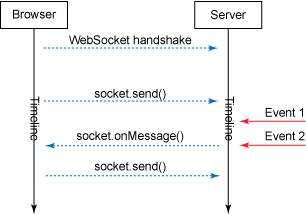
\includegraphics[scale=0.75]{websockets-flow.jpg}
  \caption[Zasada działania protokołu Web Sockets]{Zasada działania protokołu Web Sockets}
\end{figure}

Protokół Web Sockets został zaprojektowany dla przeglądarek internetowych, natomiast może być użyty w jakiejkolwiek aplikacji. Opiera się na protokole HTTP do czasu przełączenia za pomocą \emph{Upgrade Request} do etapu \emph{handshake}, a następnie na właściwą wymianę danych. Aby ustanowić połączenie w protokole Web Sockets, klient wysyła żądanie w protokole HTTP:

\lstset{language=Octave}
\begin{lstlisting}
GET /chat HTTP/1.1
Host: server.example.com
Upgrade: websocket
Connection: Upgrade
Sec-WebSocket-Key: dGhlIHNhbXBsZSBub25jZQ==
Origin: http://example.com
Sec-WebSocket-Protocol: chat, superchat
Sec-WebSocket-Version: 13
\end{lstlisting}

Klient wysyła nagłówek \lstinline{Sec-WebSocket-Key} o wartości będącej wartością losową zakodowaną jako base64\footnote{Jeden ze sposobów kodowania ciągów bajtów}.

Serwer wysyła odpowiedź \emph{101 Switching Protocols}:

\lstset{language=Octave}
\begin{lstlisting}
HTTP/1.1 101 Switching Protocols
Upgrade: websocket
Connection: Upgrade
Sec-WebSocket-Accept: s3pPLMBiTxaQ9kYGzzhZRbK+xOo=
Sec-WebSocket-Protocol: chat
\end{lstlisting}

W odpowiedzi na nagłówek \lstinline{Sec-WebSocket-Key} serwer odsyła nagłówek \lstinline{Sec-WebSocket-Accept} o wartości będącą równą:

\vspace*{1\baselineskip}
\lstinline{base64(sha1( klucz ))}
\vspace*{1\baselineskip}

Wartość \emph{klucz} to sklejenie ciągu znaków pochodzących z wartości \lstinline{Sec-WebSocket-Key} oraz stałej, ustalonej wartości \lstinline{258EAFA5-E914-47DA-95CA-C5AB0DC85B11}.

Od tego momentu rozpoczyna się transmisja w protokole Web Socekts, w którym przesyłane są ramki w trybie full-duplex:

\begin{figure}[H]
  \centering
    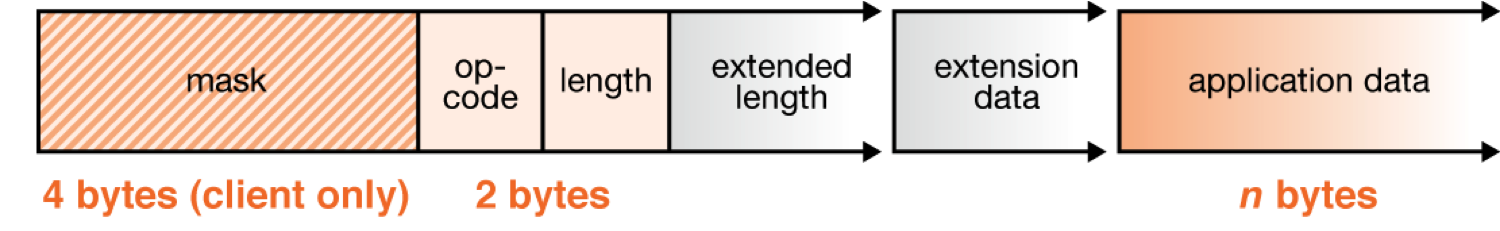
\includegraphics[scale=0.65]{WebSocketFrame.png}
  \caption[Ramka protokołu Web Sockets]{Ramka protokołu Web Sockets}
\end{figure}

\subsection{Skalowanie}
\label{subsub:scalability}

Podczas budowy systemu zauważono konieczność skalowania aplikacji przy jednoczesnym dostępie wielu użytkowników. Aby odciążyć serwer gry przy rozsyłaniu komunikatów o stanie gry do wszystkich podłączonych klientów, można wprowadzić warstwę pośrednią w postaci węzłów odpowiedzialnych za utrzymanie połączeń z klientami i przekazywanie im zstępująco i wstępująco wiadomości. Klienci łączą się bezpośrednio z węzłami pośrednimi (jak zobrazowano na diagramie w dodatku \ref{app:network_diagram_app} oraz \ref{app:pong_comp_diagram}). Za rozłożenie\footnote{Rozumiane jako równomierne zbalansowanie} ruchu sieciowego pomiędzy węzłami odpowiedzialny jest Load Balancer.

Rozróżniane są Load Balancery w dwóch kategoriach w zależności od warstwy działania w modelu sieciowym ISO/OSI:
\begin{itemize}
	\item Działające w warstwie 4. - sieciowej, tzw. sprzętowe (ang. \emph{hardware L4 load balancing}). Analizuje ramki ruchu sieciowego, szybkie w działaniu.
	\item Działające w warstwie 7. - aplikacji, tzw. programowe (ang. \emph{software L7 load balancing}). Pozwala na zaawansowaną analizę logiczną ruchu sieciowego, tańsze, ale wolniejsze.
\end{itemize}

Znanym programowym load balancerem jest HAProxy, który umożliwia podzielenie ruchu pomiędzy bliźniacze aplikacje przy użyciu kilku algorytmów\cite{haproxy-conf}:

\begin{description}
  \item[roundrobin] \hfill \\
  Algorytm zakłada wybór serwera na zasadzie karuzeli, jeden po drugim, uwzględniając przypisane wagi. Sprawiedliwy dla krótko trwających połączeń o przybliżonym czasie obsługi, np. większość żądań w protokole HTTP.
  \item[leastconn] \hfill \\
  W algorytmie wybierany jest serwer, który w danym momencie posiada najmniej otwartych połączeń. Sprawiedliwy dla długo trwających połączeń o niejednostajnym czasie obsługi, np. LDAP, połączenia serwerów bazodanowych.
  \item[source] \hfill \\
  W algorytmie adres IP, z którego obsługiwane jest połączenie, jest argumentem funkcji mieszającej, której wynik jest podzielony przez sumę wszystkich wag przypisanym serwerom pomiędzy którymi przydzielany jest ruch. Dzięki temu jeden użytkownik zawsze trafi na ten sam serwer.
  \item[uri] \hfill \\
  W algorytmie adres \emph{URI}\footnote{Część adresu URL przez znakiem zapytania} jest argumentem funkcji mieszającej, której wynik jest podzielony przez sumę wszystkich wag. Zapewnia to, że żądania z danego adresu trafią zawsze na jeden serwer. Strategia przydatna do zwiększenia ograniczonej pamięci cache uwzględniającej jako klucz skojarzeniowy adresy URI, aby zwiększyć liczbę trafień do pamięci cache (ang. \emph{cache rate}).
  \item[url param] \hfill \\
  Analogicznie do uri, natomiast argument funkcji mieszającej stanowi jeden, wybrany \emph{url param}\footnote{Część adresu URL po znaku zapytania}.
\end{description}

\subsection{CDN - Content Delivery Network}
\label{subsub:cdn}

\subsubsection{Serwowanie statycznej treści}

Aby zmniejszyć czas ładowania statycznych części składowych stron internetowych, umieszcza się je na wielu serwerach CDN\footnote{Content Delivery Network}. Celem ma być szybszy dostęp do statycznych treści, np. wybór najbliższego geograficznie serwera lub serwera, który ze względu na uszkodzenia sieci odpowiada szybciej względem innych serwerów.

W ramach pracy dyplomowej skonfigurowany został serwer CDN oparty na Varnish Cache, który udostępnia mechanizm możliwości umieszczenia odpowiedzi HTTP bezpośrednio w pamięci RAM, aby przy ponownym połączniu nie nastąpił odczyt z dysku lub uruchomienie aplikacji w celu wygenerowania odpowiedzi HTTP. Model, w którym działa Varnish, nazywa się man-in-the-middle, a wykorzystany jest mechanizm \emph{reverse proxy}.

\subsubsection{Reverse Proxy w protokole HTTP}

W przypadku rozkładu ruchu korzysta się z serwerów proxy, które przekazują żądanie klientów na inne serwery. W przypadku optymalizacji serwowania statycznej treści (ang. \emph{static content delivery}) korzysta się z odwrotnego modelu - \emph{reverse} proxy. Przyglądając się możliwościom wykorzystania zapamiętywania odpowiedzi wygenerowanej przez serwer w protokole HTTP\cite{http-rfc}\footnote{\cite{http-rfc}, rozdział \emph{Caching in HTTP}} przez klientów, dla których pamięć cache jest indywidualna i serwowanie statycznej treści odbywa się dla każdego z nich indywidualnie, powstaje wątpliwość, czy można zapobiec nadmiernym odczytom z dysków.

Protokół HTTP zapewnia dwa modele zapamiętywania w pamięci cache przesłanej odpowiedzi:

\begin{description}
  \item[Expiration model] \hfill \\
  Model oparty o czas ważności odpowiedzi. Serwer wraz z odpowiedzią przesyła w nagłówku \lstinline{Expires} datę jej ważności, która jest skojarzona bezpośrednio z adresem URL, do którego przesłane zostało żądanie. W przypadku ponownego wysłania zapytania, przeglądarka użytkownika może wczytać treść odpowiedzi z lokalnej pamięci cache, aby skrócić czas ładowania strony, o ile czas ważności odpowiedzi nie minął.
  \item[Validation model] \hfill \\
  Model oparty o poprawność odpowiedzi. Serwer wraz z odpowiedzią przesyła w nagłówku \lstinline{Last-Modified} datę ostatniej modyfikacji odpowiedzi (np. datę modyfikacji pliku). Przy ponownym żądaniu przeglądarka wysyła zapytanie o plik pod wskazany adres URL wraz z uprzednio przesłaną datą. W przypadku, gdy data jest taka sama, serwer odpowiada wyłącznie nagłówkiem \lstinline{304 (Not Modified)} nie przesyłając w odpowiedzi treści statycznej treści. Umożliwia to zredukowanie liczby odczytów z dysku serwera.
\end{description}

W modelu reverse-proxy zamiast odwoływać się do lokalnych pamięci cache użytkowników, kreuje się wirtualnego, globalengo użytkownika z pamięcią cache, który jest widziany jako serwer dla wszystkich klientów, w ten sposób pamięć cache jest wspólna dla wszystkich, co dodatkowo redukuje obciążenie serwera związane z odczytem statycznych plików z dysków. Globalna pamięć może być przechowywana w pamięci RAM, aby szybciej dostarczać treści.

\begin{figure}[H]
  \centering
    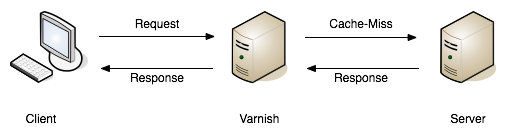
\includegraphics[scale=0.75]{varnish-miss.png} \\
    Rysunek przedstawia przypadek, gdy Varnish nie znalazł wpisu w cache oraz przekazuje żądanie do serwera aplikacji, aby otrzymać odpowiedź.
  \caption[Varnish cache miss]{Varnish cache miss}
\end{figure}

\begin{figure}[H]
  \centering
    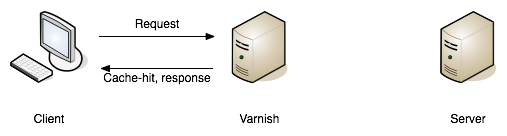
\includegraphics[scale=0.75]{varnish-hit.png} \\
    Rysunek przedstawia przypadek, gdy Varnish znalazł wpis w cache, nie jest konieczne przekazanie połączenia do serwera aplikacji, odpowiedź jest wczytywana prosto z pamięci RAM.
  \caption[Varnish cache hit]{Varnish cache hit}
\end{figure}


\subsection{Wybór komputera wyświetlającego obraz na ekranie}
\label{sec:Komputer wyświetlający obraz na ekranie}

Klient to komputer podłączony bezpośrednio do ekranu wyświetlającego obraz. Istotnymi cechami takiego urządzenia są przede wszystkim:
\begin{itemize}
	\item niska cena
	\item wystarczająca moc obliczeniowa do uruchomienia przeglądarki, oraz prostej gry w technologi Flash, lub HTML5
	\item duża dostępność
	\item mały rozmiar
\end{itemize}

Głównym zadaniem klientów jest komunikacja serwerem poprzez sieć Ethernet w celu wyświetlania obrazu na podłączonym do klienta ekranie, oraz możliwość sterowania urządzeniami wejścia (klawiatura, myszka) poprzez udostępniony interfejs w sieci Ethernet.

Jeśli chodzi o wybór architektury procesora wybór był całkiem prosty, za sprawą sporej liczby dostępnych urządzeń dostępnych w tej architekturze (32 bitowa architektura ARM\footnote{Advanced RISC Machine} jest najczęściej stosowaną architekturą w urządzeniach mobilnych\cite{acm}), jak i uzasadnioną ich popularnością. Architektura ARM cechuje cię niskim poborem energii, dużą niezawodnością w systemach wbudowanych, oraz dla praktycznie wszystkich dostępnych na rynku procesorów możliwością instalacji w pełni funkcjonalnego systemu operacyjnego.
Procesory oparte o architekturę ARM przetwarzają instrukcje z wykorzystaniem mechanizmu potokowania. Procesor może wykonywać trzy rodzaje instrukcji:
\begin{itemize}
	\item 32-bitowe ARM
	\item 64-bitowe ARM (Apple A7)
	\item 16-bitowe Thumb (oraz Thumb2)
\end{itemize}

\par
Firma ARM projektuje rdzenie procesorów i sprzedaje je producentom. Producenci z kolei tworzą urządzenia typu SoC\footnote{System on Chip} - dodawane są bloki funkcyjne, jednostki wektorowe czy procesory sygnałowe. Istnieje też spora lista firm, które projektują swoje rdzenie wykorzystujące zbiór instrukcji ARM m.in. Apple, XScale, czy Faraday.

\par
Istotną cechą, którą powinien posiadać procesor ARM jest jednostka MMU\footnote{Memory Managment Unit}. Jest to jednostka odpowiadająca za dostęp do zewnętrznej pamięci, translacje adresu wirtualnego na fizyczny, oraz kontroli uprawnień dostępu do pamięci. Wiele rdzeni ARM nie jest wyposażonych w tą jednostkę, która staje się obligatoryjna podczas gdy chcemy zainstalować system operacyjny Linux. 
\par

Po wyborze architektury procesora należy wybrać rodzinę procesora. Rodzina Cortex jest kolejną generacją procesorów po ARM7, ARM9, czy ARM11.

\begin{figure}
\begin{center}
	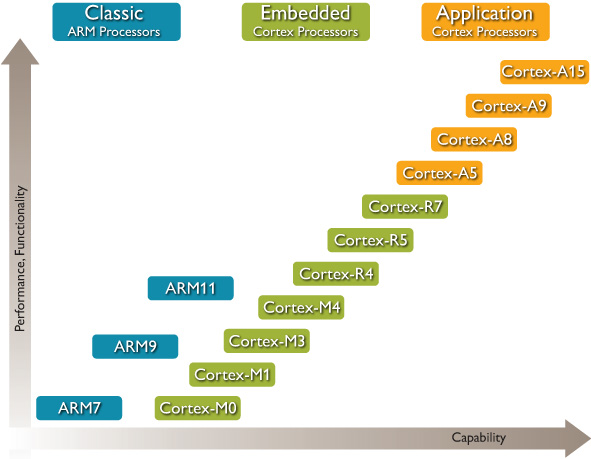
\includegraphics[scale=0.6]{ARM_Comparison}
\end{center}
\caption{Porównanie rodzin architektury ARM}
\label{fig:ARM_Comp}
\end{figure}

Zgodnie z tym co można zauważyć na rysunku~\ref{fig:ARM_Comp} architektura Cortex jest rodziną cechującą się wyższym od swoich poprzedników współczynnikiem wydajności na cykl zegara i niższym zużyciem energii.

Na rynku można wyodrębnić 3 główne chipy bazujące na architekturze ARM:
\begin{itemize}
	\item Allwinner (sunxi)
	Przykładowe produkty:
	\begin{itemize}
		\item Hackberry A10
		\item MK802
	\end{itemize}

	Chipy Allwinnera charakteryzują się stosunkowo najniższą ceną, oba przedstawione wyżej modele bazują na rdzeniu Cortex-A8 taktowane zegarem 1GHz, oraz dysponujące 1GB pamięci operacyjnej. Wyposażone są także w procesor graficzny ARM Mali 400
	
	\item Freescale i.MX6 (imx)
	Przykładowe produkty:
	\begin{itemize}
		\item MarS
		\item IMX53QSB
	\end{itemize}
	\item TI OMAP3/4
	Przykładowe produkty:
		\begin{itemize}
			\item Beaglebone Black
			\item Panda Board
		\end{itemize}
	Ta rodzina zyskała bardzo dużą popularność. Chipy OMAP3 wyposażone są w zmiennoprzecinkową jednostkę oraz zestaw instrukcji wektorowych NEON. Główną cechą tego rozwiązania jest dużo wydajność operacji przy zachowaniu prostoty ich programowania.
\end{itemize}

\subsection{System operacyjny dla komputera wyświetlającego obraz na ekranie.}

Nie dysponując zbyt dużą mocą obliczeniową, małą pamięcią operacyjną, oraz niewielką przestrzenią dyskową należy dobrze dobrać, oraz skonfigurować system operacyjny. Do tego celu wybrano dystrybucje linuksa - Debian. Cechuje się ona przede wszystkim wysoką stabilnością (bardzo często wybierana jako system serwerowy), oraz sporą społecznością programistów rozwijających tą dystrybucje co przekłada się na mnogość dostępnych pakietów przygotowanych specjalnie dla tej wersji systemu Linux. Wreszcie system Debian jest wysoce konfigurowalny - oparty o jądro Linux, daje użytkownikowi możliwość zbudowania systemu od podstaw. Dlatego też jako system docelowy i główny wybraliśmy dystrybucje Debian.

\begin{figure}
\begin{center}
    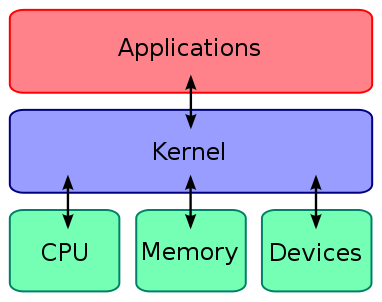
\includegraphics[scale=0.5]{kernel}
\end{center}
\caption{Działanie jądra systemu Linux}
\label{fig:kernel}
\end{figure}

Jądro \footnote{ang. \emph{Kernel}} systemu Linux jest centralnym miejscem systemu operacyjnego. Jak zaprezentowano na rysunku ~\ref{fig:kernel} jest ono najniżej usytuowaną warstwą systemu operacyjnego odpowiadającą za komunikację z procesorem, pamięcią, czy urządzeniami zewnętrznymi. Kernel m.in. przydziela odpowiednią ilość pamięci operacyjnej dla każdej aplikacji, obsługuje komunikaty i komunikacje między procesorową.

Pierwotnym twórcą jądra Linux jest programista pochodzenia duńskiego Linus Torvalds, natomiast obecnie jądro systemu Linux jest rozwijane przez programistów z całego świata. Jego aktualną wersje można pobrać z oficjalnego otwartego repozytorium github.


\par








\subsection{Serwer zarządzania infrastrukturą}

Większość języków programowania, technologii spełnia wymagania niefunkcjonalne dla serwera zarządzania infrastrukturą. Z racji tego, że wymagania niefunkcjonalne dla serwera zarządzania infrastrukturą nie zawężały mocno kręgu poszukiwań, dodatkowymi kryteriami jakie zostały narzucone były:

\begin{itemize}
	\item skalowalność
	\item szybkość wykonania (ang. \emph{execution time})
	\item szybkość programowania (ang. \emph{development time})
\end{itemize}

\subsubsection{Język programowania}

Biorąc pod uwagę powyższe wymagania wybrano język scala.


\begin{description}
	\item[Dlaczego scala?] \hfill \par 
	\begin{description}
		\item[Zwięzła] \hfill \par
			Programy w scali zajmują ok. 30\%-50\% mniej kodu aniżeli te same napisane w języku Java.
		\item[Portowalna] \hfill \par
			Kod napisy w języku scala kompilowany jest do kodu bajtowego, i uruchamiany na JVM\footnote{Wirtualna Maszyna Javy ang. \emph{Java Virtual Machine}}. Dzięki czemu może korzystać z bibliotek napisanych w języku Java.
		\item[Hybrydowa] \hfill \par
			Język scala łączy w sobie dwa najpopularniejsze paradygmaty programowania jest zarazem imperatywna jak i w pełni funkcjonalna.
		\item[Statyczne typowana] \hfill \par
			Scala jest statycznie typowana w przeciwieństwie do języków skryptowych takich jak Ruby, czy Python, co wprowadza większy porządek w kodzie, bezpieczne refaktoryzowanie, czy pomaga w generowaniu lepszej dokumentacji. Dodatkowo w przeciwieństwie do języka java, scala posiada świetny mechanizm domniemywania typów.
		\item[Skalowalna] \hfill \par
			Dostarcza wiele funkcjonalności usprawniających równoleglizacje kodu, przede wszystkim ma niezmienne typy, i równoległość opartą na modelu aktorów (eng. \emph{actor based concurrency}).
	\end{description}
\end{description}


\subsubsection{Framework}

Jako framework została wybrany Play! 2.

\begin{description}
	\item[Czym jest Play! ?]\hfill \\
		W skład frameworka Play! prócz samej biblioteki programistycznej wchodzi m.in. wydajny serwer HTTP JBoss Netty, wiele skryptów do zarządzania aplikacją, oraz wbudowany kompilator Java. Framework play jest oparty na wzorcu MVC\footnote{Model Widok Kontroler ang. \emph{Model View Controller}}. Play nie zyskał zbyt wielkiej popularnej w wersji 1.x, natomiast od momentu kiedy został przepisany na język scala (od wersji 2.x) jest on coraz częściej wybierany przez programistów i analityków. 
	\item[Dlaczego Play! ?]\hfill \\
		\begin{description}
			\item[bezstanowy] \hfill \\ nie ma wydzielonego fragmentu przestrzeni na serwerze, która jest ściśle powiązana z zalogowanym użytkownikiem. Na pierwszy rzut oka wydaję się to być wadą, natomiast niesie to ze sobą szereg plusów jak np. świetna skalowalność aplikacji (nie ma potrzeby zapewniania zgodności spójności sesji pomiędzy serwerami).
			\item[reaktywny] \hfill \\ oparty o programowanie reaktywne\footnote{ang. \emph{Reactive Programming} paradygmat programowania zakładający że oprogramowanie jest zawsze responsywne na nadchodzące zdarzenia.}		
			\item[zorientowany na zdarzenia, a nie żądania] \hfill \\ wątek nie jest przypisany od początku do końca do jednego żądania
			\item[przyjazny dla developera] \hfill \\ po przeładowaniu przeglądarki, zmieniony kod jest rekompilowany, a ewentualne błędy podczas uruchomienia są wyświetlane w przeglądarce wraz z stosem wywołań.
			\item[skalowalny] \hfill \\ od wersji 2.0 oparty na modelu aktorów, co daje wysoką skalowalność. 
		\end{description}
\end{description}







\newpage
\section{Narzędzia}
\label{sec:tools}

\subsection{Narzędzia wspomagające zarządzanie projektem}

\subsubsection{GIT}
\label{sub:GIT}
GIT to rozproszony system kontroli wersji. System ten pozwala na bezproblemową synchronizację pracy między stacjami roboczymi. Dzięki temu, że jest on rozproszony, nie jest konieczne wyznaczanie głównego serwera, przez który synchronizowany jest kod źródłowy, a każdy z klientów może pełnić rolę serwera do którego wysyłane są zmiany plików objętych systemem kontroli wersji.

Przy realizacji pracy dyplomowej GIT pomógł rozwiązywać konflikty w treści kodu źródłowego, ciągłe nadpisywanie treści plików powstałe w wyniku pracy kilku osób. Do przechowania kodu źródłowego na serwerze zdalnym wykorzystana została darmowa powierzchnia serwisów GitHub oraz Bitbucket. Na Githubie umieszczone zostały aplikacje stworzone w ramach projektu oraz praca dypomowa napisana w LaTeX-u.


\subsubsection{Asana}
\label{sub:Asana}

Praca w zespole wymagała skorzystania narzędzia wspomagającego komunikację oraz kontrolę wykonywania zadań. Asana to system zarządzania projektem umożliwiający rozdzielanie zadań pomiędzy członków zespołu przypisanych do projektu, śledzenie postępów prac, ustalanie przypomnień oraz terminów. System wspomaga komunikację, dzieli obszary zainteresowań na podprojekty, umożliwia oznaczenie zagadnień słowami kluczowymi oraz udostępnia wyszukiwarkę. Narzędzie oparte o model SaaS (ang. Software as a Service) dostępne przez przeglądarkę internetową bez konieczności instalacji oprogramowania.

W projekcie narzędzie wykorzystane zostało do monitorowania postępów prac oraz do tworzenia bazy wiedzy.

\subsection{Narzędzia programistyczne}

\subsubsection{Vim}
\label{sub:Vim}
Prawdopodobnie najpopularniejszy konsolowy edytor tekstu. Vim jest klonem edytora vi, z wieloma nowymi funkcjami. Przede wszystkim jest to modalny edytor tesktu tzn. że posiada więcej niż jeden tryb pracy (INPUT, COMMAND, VISUAL). Dzięki swojej prostocie, szybkości, oraz mnogości wtyczek ten konsolowy edytor jest wciąż bardzo popularny i używany w zastępstwie wielu zintegrowanych środowisk programistycznych jak np. Eclipse czy VisualStudio.  

\subsection{Technologia wykorzystana w pilotach}

\subsubsection{jQuery Mobile}
\label{subsub:tool-jquery-mobile}

Brak respektowania standardów (podsekcja \ref{subsec:w3c-touch-events-implementations}) stwarza problemy związane z obsługą gestów na urządzeniach mobilnych. Aby zapewnić poprawne funkcjonowanie, należy śledzić zmiany wprowadzane w implementacjach przeglądarek przez producentów oraz ewentualne zmiany w standardach. W projekcie wykorzystana została biblioteka \emph{jQuery Mobile} posiadająca dużą społeczność\footnote{Ponad 10 tyś poprawek, 36 wersji, 204 osób wnoszących wkład w rozwój biblioteki [Stan na 22 grudnia 2013]}. Wśród wspieranych przeglądarek znajdują się wymienione jako niewspierające standardu z podsekcji ~\ref{subsec:w3c-touch-events-implementations}.

Biblioteka wykorzystywana w zakresie poruszania punktów dotyku definiuje \emph{wirtualną mysz} (oznaczoną \lstinline{vmouse}) jako dotyk na urządzeniu mobilnym. Zdarzenia obsługujące wirtualną mysz są wyzwalane dla myszy komputerowej oraz dla panelu dotykowego.

Zdarzenie \lstinline{vmousemove} symuluje zdarzenia \lstinline{onmousemove} oraz \lstinline{touchmove}. Przykład użycia:

\lstset{language=JavaScript}
\begin{lstlisting}
$(document).on('vmousemove', function(e) {
	// Zapobieganie dalszej propagacji zdarzenia
	// po przechwyceniu, strona nie bedzie przewijana.
	e.preventDefault();
	
	// Pobieranie pozycji kursora z obiektu zdarzenia.
	var x = e.pageX
	var y = e.pageY
	
	console.log(x, y) // wypisz dane na konsoli
})
\end{lstlisting}

\subsubsection{Użycie biblioteki basket.js}
\label{subsub:tools-basketjs}

Zgodnie z analizą dokonaną w rozdziale \ref{subsub:webstorage-performance}, wszystkie skrypty JavaScript pilota są umieszczone z lokalnej pamięci przeglądarki internetowej Web Storage na telefonie komórkowym. W tym celu opracowana została biblioteka \emph{basket.js} oferująca asynchroniczne ładowanie kodu JavaScript z rozwiązywaniem zależności między plikami oraz roztrzyganiem wyścigów\footnote{W asynchronicznym modelu programowania kolejne kawałki kodu nie wykonują się sekwencyjnie, co może doprowadzić do błędów wynikających z zależności między nimi.}.Biblioteka basket.js jako interfejsu dla programisty używa wzorca projektowego \emph{Promise}.

Dla ułatwienia zarządzania kodem wykonującym się asynchronicznie stosuje się najczęściej trzy wzorce projektowe: Callback, Events i Promise.

\begin{description}
  \item[ Wzorzec Callback] \hfill \\
  Polega na zarejestrowaniu funkcji, do której przechodzi się zaraz po wykonaniu asynchronicznej operacji. Przykład:
  \lstset{language=Octave}
  \begin{lstlisting}
  database.query("SELECT * FROM table;", function(data), {
  	console.log(data) // wiersze do wypisania
  })
  \end{lstlisting}
  \lstinline{function(data)} to sygnatura anonimowej\footnote{Anonimowej - nie posiadającej identyfikatora, w konsekwencji nie można jej ponownie użyć.} funkcji. Zamiast sygnatury może zostać podany identyfikator wcześniej zadeklarowanej funkcji. Minusem tego rozwiązania jest fakt, że istnieje tylko jedna funkcja, która reaguje na zakończenie operacji, co w niektórych przypadkach może stwarzać kłopoty. Drugim minusem tego rozwiązania jest to, że zarówno w przypadku błędu, jak i powodzenia, wykonywana jest ta sama funkcja.
  \item[Wzorzec Events] \hfill \\
  Jako środek zaradczy na reagowanie tylko jedną funkcją na zakończenie operacji przychodzi wzorzec projektowy \emph{Events} (ang. zdarzenia), który domyślnie implementuje funkcję, która w pętli iteracyjnie wykonuje wszystkie funkcje zarejestrowane jako callback. Innymi słowy, istnieje wiele funkcji callback, które reagują na dane zdarzenie, na przykład:\\

  

  Wzorzec projektowy nie rozwiązuje natomiast problemu, iż w przypadku powodzenia lub niepowodzenia operacji, wykonuje się ten sam zestaw funkcji callback. Z wykonania wielu funkcji callback w systemach, gdzie mogą one być wykonywane równolegle, wzorzec projektowy posiada wadę wynikającą z synchronizacji funkcji.
  \lstset{language=Octave}
  \begin{lstlisting}
  var funkcja1 = function() {
  	console.log('zaszlo zdarzenie klikniecia')
  }
  element.on('click', funkcja1)
  element.on('click', function() {
  	console.log('zaszlo zdarzenie klikniecia')
  })
  \end{lstlisting}
  \item[Promise] \hfill \\
  Jest to wzorzec projektowy deklarujący strukturę funkcji reprezentującą zdarzenie, które zajdzie w przyszłości. Pozwala to na wykonywanie funkcji zarówno jako Events, jak i Callback, bowiem obiekty mogą być łączone w synchroniczny łańcuch.
\end{description}

Przykład użycia biblioteki basket.js jako wzorca projektowego Promise:

\lstset{language=JavaScript}
\begin{lstlisting}
basket
    .require(
		{ url: 'assets/js/jquery-1.10.2.min.js' },
		{ url: 'assets/js/socket.io.js' }
	)
    .then(function() {
        basket.require({url:'assets/js/jquery.mobile-1.3.2.min.js'});
    })
	.then(function() {
        basket.require({ url: 'app.js' });
    })
	.then(function() {
	 	// ...
	})
});
\end{lstlisting}

Funkcja \lstinline{require} na rzecz obiektu \lstinline{basket} zwraca obiekt Promise, który uruchamia równolegle trzy funkcje callback. Funkcje callback również mogą zwracać obiekty Promise, tworząc synchroniczny łańcuch.

\subsection{Technologia wykorzystywana w części serwerowej}
\label{sub:tool-server-technology}

Część serwerowa infrastruktury została napisana w środowisku \emph{Node.js}, stworzonym przez Ryana Dahla w 2009 roku. Node.js używa składni skryptowego\footnote{Kod języków skryptowych wykonywany jest wewnątrz jakiejś aplikacji/środowiska w odróżnieniu od programów napisanych w językach nieskryptowych, które kompilują się i stanowią aplikację.} języka JavaScript znanego z tworzenia dynamicznych elementów stron internetowych. Kod JavaScript, choć wykonuje się w ramach przeglądarki internetowej, w Node.js uruchamiany jest po stronie serwera. Technologia umożliwia uzyskanie dużej przepustowości, zapewniającej nieblokujące wykonywanie operacji wejścia/wyjścia (ang. \emph{non-blocking I/O}). Podejście to nazywa się programowaniem asynchronicznym (jest ono opisane w podrozdziale \ref{subsub:asyncprogramming}).

Wybór platformy obsługującej programowanie asynchroniczne jest jednoznaczny ze względu na specyfikę aplikacji. Jeżeli program byłby napisany w modelu synchronicznym, procesor przeznaczałby większość czasu na oczekiwanie na dane z sieci zawieszając (ang. \emph{idle}) swoją pracę na funkcjach wejścia/wyjścia. Tymczasem, aby zwiększyć możliwości (uruchomienie tysięcy operacji I/O jednocześnie) korzysta się z asynchronicznego, nieblokującego podejścia pisania aplikacji zprzy użyciu pętli zdarzeń uruchomionej w pojedynczym wątku. Podejście jest odpowiednie do czasu, gdy program nie wykonuje złożonych czasowo operacji, które to mogłyby zawiesić działanie pętli komunikatów uruchomionej w pojedynczym wątku. Większość operacji w stworzonej aplikacji to przekazywanie struktur danych i praca w sieci.

\subsubsection{Synchroniczny i imperatywny model programowania}

W porównaniu do programowania asynchronicznego przedstawione krótko zostanie programowanie imperatywne, będące paradygmatem programowania\cite{programming-paradigms}, które opisuje kod programu jako sekwencyjnie wykonywany ciąg instrukcji zmieniający stan programu (rejestrów, pamięci). Takie wyobrażenie przebiegu wykonania programu jest de facto tożsame z fizyczną realizacją kodu maszynowego na komputerze. W tym modelu przebieg programu możemy zdefiniować jako ciąg następujących po sobie instrukcji, dzięki czemu ten przebieg jest przewidywalny, bowiem wykonując bieżącą instrukcję można założyć, ze poprzednia się zakończyła powodzeniem, a jej wyniki są dostępne do użycia. Implikuje to, że wykonywanie każdej operacji jest blokujące. Rozwiązaniem tego problemu jest uruchamianie przebiegu programu w wątkach, mogących komunikować się między sobą lub uruchomienie programu jako nowy proces w systemie operacyjnym\footnote{Te zabiegi powodują narzut czasowy związany z przełączaniem kontekstu pracy procesora w postaci odłożenia stanu rejestrów, mapy pamięci, rejestrów stosu, FPU itd.}.

\begin{figure}[ht]
\centering
\begin{minipage}[b]{0.45\linewidth}
  \label{fig:syncprogramming-flow}
  \caption[Programowanie synchroniczne - przebieg instrukcji programu w czasie]{Programowanie synchroniczne - przebieg instrukcji programu w czasie}
  \centering
    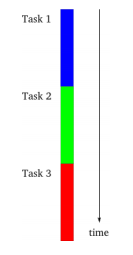
\includegraphics[scale=0.5]{syncprogramming-flow.png}
\end{minipage}

\begin{minipage}[b]{0.45\linewidth}
\label{fig:syncprogramming-threads}
  \caption[Programowanie synchroniczne - wątki]{Programowanie synchroniczne - wątki}
  \centering
    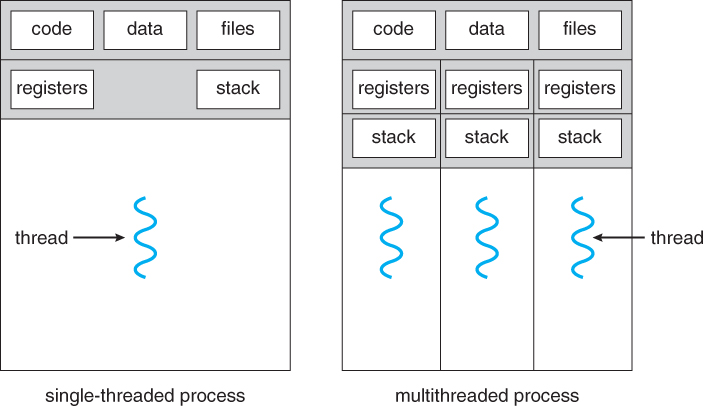
\includegraphics[scale=0.5]{syncprogramming-threads.jpg}
\end{minipage}

\begin{minipage}[b]{0.45\linewidth}
\label{fig:syncprogramming-waiting}
  \caption[Programowanie synchroniczne - operacje blokujące]{Programowanie synchroniczne - operacje blokujące}
  \centering
    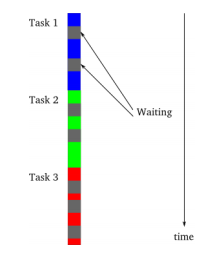
\includegraphics[scale=0.5]{syncprogramming-waiting.png}
\end{minipage}
\end{figure}

\subsubsection{Asynchroniczny model programowania}
\label{subsub:asyncprogramming}

Asynchroniczny model programowania oparty jest na programie uruchomionym w jednym wątku. Znany jest z frameworków graficznych interfejsów użytkownika GUI (na przykład WinApi). W uproszczeniu, budowa programu to nieskończona pętla oraz kolejka operacji odłożona na stos. Z każdym przebiegiem pętla sprawdza w kolejce operacji, czy możliwe są do wykonania jakieś operacje, jeżeli tak, uruchamiane są procedury obsługi (ang. \emph{handlers} lub \emph{callbacks}). Umożliwia to realizację wielu operacji, które oczekują na wyniki, bez blokowania pracy całego programu.

\begin{figure}[H]
  \caption[Event loop w asynchronicznym modelu programowania]{Event loop w asynchronicznym modelu programowania}
  \centering
    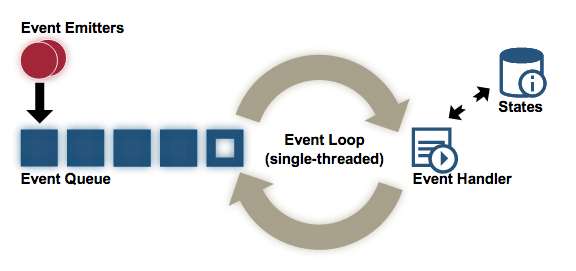
\includegraphics[width=\linewidth]{asyncprogramming-loop.png}
\end{figure}

Realizacja niskopoziomowa to użycie funkcji \lstinline{select()} (zarówno systemów POSIX jak i Windows), deskryptorów \lstinline{/dev/poll}, kqueue, poll i epool. Warta rozpoznania jest biblioteka \emph{libevent}\footnote{\url{http://libevent.org/}}, która zakłada abstrakcję na użyte mechanizmy z punktu widzenia programisty\cite{programming-async-sockets}.

Funkcja \lstinline{select()} przyjmuje za parametry deskryptory oraz maksymalny czas upływu. Zwraca wartość jeżeli a) upłynie zdefiniowany czas lub b) gdy w deskryptorze (reprezentującym plik, urządzenie, gniazdo sieciowe lub strumień danych) zajdą zmiany - będzie dostępny do zapisu lub są dostępne dane do odczytu:

\lstset{language=C}
\begin{lstlisting}
#include <sys/time.h>
#include <sys/types.h>
#include <unistd.h>

int select(int numfds, fd_set *readfds, fd_set *writefds,
           fd_set *exceptfds, struct timeval *timeout);
\end{lstlisting}

W przeciwieństwie do synchronicznego modelu w programowaniu imperatywnym, model asynchroniczny wypada korzystniej, gdy\cite{programming-async}:

\begin{enumerate}
  \item Zadania są zupełnie niezależne od siebie, nie jest konieczna komunikacja między nimi, ani oczekiwanie na rezultaty.
  \item Zadania wykonują wiele operacji wejścia/wyjścia (I/O) powodujących, że program synchroniczny zostaje zawieszony do momentu otrzymania rezultatu, wtenczas może wykonywać inne zadania.
\end{enumerate}

Zatem program napisany asynchronicznie blokuje swoje działanie tylko wtedy, gdy nie ma zadań do wykonania i nie jest możliwy dalszy postęp przebiegu programu (dlatego jest nazywany nieblokującym). Przy wykonaniu wielu blokujących zadań program napisany asynchronicznie może być znacznie szybszy spędzając mniej czasu na czekaniu na wyniki, a wykonując wiele pojedynczych zadań podczas przebiegu pętli.

\subsubsection{Zasada działania Node.js}
\label{sub:tool-server-nodejs}

Node.js jest środowiskiem używającym składni skryptowego języka JavaScript\footnote{Po kliku nieudanych próbach implementacji w C, Lua,  Haskell, twórca Node.js Ryan Dahl, po pojawieniu się Google JavaScript Engine V8 zdecydował się na jego użycie}, udostępniającym mechanizmy programowania asynchronicznego opartego o wywołania funkcji \emph{callbacks}. Node.js działa w pojedynczym wątku opartym o pętlę zdarzeń obsługiwanych przez procedury obsługi (callbacks). Środowisko oparte jest na projekcie opensource \emph{V8 Javascript Engine} wydanym przez Google, który (w odróżnieniu od innych) kompiluje JavaScript do kodu maszynowego\footnote{Obsługiwane platformy: IA-32, x86-64, ARM oraz MIPS ISAs} przed jego wykonaniem.

\begin{figure}[H]
  \caption[Model działania Node.js]{Model działania Node.js na przykładzie serwera HTTP}
  \centering
    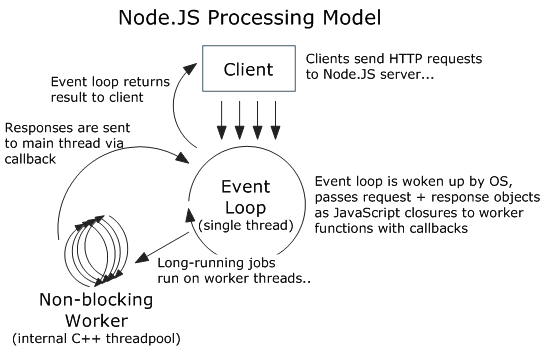
\includegraphics[scale=0.75]{nodejs-flow.png}
\end{figure}

\subsubsection{Socket.io}
\label{subsub:socketio}

Socket.io to biblioteka Node.js, która zapewnia komunikację dwukierunkową między przeglądarka użytkownika, a serwerem. Co ważne, sposób wykorzystania biblioteki zarówno po stornie serwera, jak i klienta jest taki sam. Komunikacja zapewniana jest przez wspierane sposoby opisane w podrozdziale \ref{sub:communication-methods})\footnote{http://socket.io/\#browser-support}:

\begin{enumerate}
  \item WebSocket
  \item Adobe® Flash® Socket
  \item AJAX long polling
  \item AJAX multipart streaming
  \item Forever Iframe
  \item JSONP Polling
\end{enumerate}

Przykładowy node.js kod po stronie serwera:

\lstinputlisting[language=JavaScript]{assets/src/socketio-example-server.js}

Powyższy kod uruchamia serwer nasłuchujący na porcie 8081, i przyjmuje zgłoszenia. Gdy klient się podłączy, dodawany jest callback na rzecz obiektu klienta \lstinline{socket} na wiadomość nazwaną \emph{the message from client}, który jest wykonywany, gdy wiadomość o takim identyfikatorze nadejdzie, za pomocą konstrukcji \lstinline{socket.on('the_message_from_client', function(data)}. Wysyłanie wiadomości podłączonemu klientowi odbywa się poprzez wywołanie metody emit na rzecz obiektu klienta socket \lstinline{socket.emit('the_message_from_server', function(data)} , która przyjmuje argument jako nazwę wiadomości \emph{the message from server} oraz drugi w postaci obiektu JavaScript, który zostanie zserializowany do formatu JSON i wysłany jako tekst, gdzie po stornie klienta zostanie zdeserializowany i zinterpretowany również jako obiekt JavaScript.

Przykładowy kod po stornie klienta:

\lstinputlisting[language=JavaScript]{assets/src/socketio-example-client.js}

Kod jest bliźniaczo podobny do kodu uruchamianego na serwerze. Klient ustanawia połączenie do adresu podanego jako argument funkcji \lstinline{connect}. Domyślnie używany jest protokół WebSocket ws://, można skorzystać z szyfrowanego protokołu wss://\footnote{analogiczny http:// do https://} wskazując go przed nazwę hosta. Istnieje możliwość skonfigurowania połączenia, np wskazać, czy ma zostać podjęta próba ponownego połączenia przy jego utracie.

\subsubsection{HAProxy}

Programowy serwer proxy służący do możliwie równego rozłożenia ruchu sieciowego w warstwie 7 modelu ISO/OSI pomiędzy skonfigurowane serwery.

\subsubsection{Varnish Cache}

Serwer reverse-proxy służacy do zapamiętywania odpowiedzi generowanych przez aplikacje w pamięci cache umieszczonej w RAM. Instalowany jako serwer, z którym klienci łączą się po dostarczenie treści, w przypadku, gdy Varnish nie posiada zapamiętanej odpowiedzi, połączenie jest przekazywane do docelowego serwera, aby przekazać i zapamiętać wygenerowaną przez niego odpowiedź.

\subsection{Wykorzystane technologie i narzędzia w serwerze zarządzającym infrastrukturą}

\subsubsection{SBT}

SBT (ang. \emph{Simple Build Tool}) to narzędzie służące do budowania projektów, rozwiązywanie zależności, podobne jest bardzo do bardziej znanych tego typu narzędzi jak Maven, czy Ant. Natomiast w przeciwieństwie do tych narzędzi cała konfiguracja odbywa się w jednym pliku i do tego napisanym w języku Scala. Nie jest również niezbędna dodatkowa integracja środowiska programistycznego. By dodać nową zależność do projektu, należy otworzyć plik \lstinline|Build.sbt| i dodać zależność według następującego schematu:

\begin{lstlisting}
//identyfikator grupy    %%     identyfikator artefaktu  %   wersja
"com.decodified"         %%     "scala-ssh"              %   "0.6.4"
\end{lstlisting}

Standardowo SBT korzysta tylko z publicznych standardowych repozytoriów, by dodać nowe (mogą to być repozytoria Maven czy Ivy), należy w tym samym pliku dodać je według następującego przykładu:

\begin{lstlisting}
resolvers += "spray repo" at "http://repo.spray.io"
\end{lstlisting}

\subsubsection{Akcje we frameworku Play}

W kontrolerach (które w scali są obiektami) definiowane są metody, każda z metod odpowiada za konkretną akcje, odpowiadając na żądanie użytkownika. Proszę przyjrzeć się następującemu kontrolerowi:

\begin{lstlisting}
object Application extends Controller {
  def index = Action {
    Ok("It works!")
  }
}
\end{lstlisting}

Obiekt \lstinline{Application} dziedziczy po cesze \lstinline{Controller}, która między innymi zapewnia szereg metod pomocniczych do zdefiniowania akcji. Metoda \lstinline{index} jest definiowana przez funkcję \lstinline{Action} (reprezentowana w Javie jako obiekt), która jako argument przyjmuje obiekt typu \lstinline{Request}, a zwraca z kolei obiekty typu \lstinline{Response}. 

\par

Tak zdefiniowana akcja definiuje blok kodu w sposób synchroniczny zwracający wynik, jednak aplikacje internetowe coraz częściej zorientowane są wokół usług internetowych (ang. \emph{Web Services}), które w sporej większości nie mają WSLA\footnote{ang. \emph{Web Service Legal Agreement} umowa utrzymania jakości usług. Pozwala autorom na wyszczególnienie wymagań co do usługi, oraz akcji, które powinny zostać podjęte podczas gdy te nie zostaną spełnione}.

\par

Framework Play w założeniu działa na bardzo małym zbiorze wątków, dlatego też podczas gdy dana akcja nie może odpowiedzieć natychmiastowo np. z powodu wykorzystywanej usługi internetowej czy długiego zapytania do bazy danych, wątek obsługujący daną akcje nie może zostać zablokowany, ale musi zostać zwolniony.

\begin{description}	
	\item[Future] \hfill \\
		Za pomocą zmiennej o tym typie, można uzyskać wartość, kiedy tylko będzie dostępna.
	\item[Promise] \hfill \\
		Typ Promise działa w przeciwną stronę tzn. jeżeli \lstinline{Future} jest typem konsumenta, tak \lstinline{Promise} jest typem charakterystycznym dla producenta. Za każdym razem gdy programista chcę obliczyć lub pobrać jakieś dane tworzy obiekt \lstinline{Promise}, który jest kontenerem na nowe dane. Z obiektu \lstinline{Promise} otrzymuje się obiekt typu \lstinline{Future}.
\end{description}

\begin{lstlisting}
def index = Action.async {
  val foo: Future[Foo] = getFoo()
  foo.map(f => Ok(f))
}
\end{lstlisting}

\par

W linii pierwszej powyższego listingu definiowana jest funkcja \lstinline{Action.async}. Funkcja ta powoduje, że wątek obsługujący tą akcje jest zwalniany, i system wraca do wykonania tej metody podczas gdy zmienna \lstinline{foo} zostanie pobrana/obliczona.

\par
Interesująca funkcjonalność jest zaprezentowana w linii trzeciej. Funkcja \lstinline{map} wywołana na obiekcie \lstinline{Future}, zwraca rezultat dopiero podczas gdy obiekt \lstinline{foo} zostanie uzupełniony. Mechanizm ten jest o tyle interesujący, że w innych językach programowania jest to wykonywane za pomocą funkcji \lstinline{onSuccess}. Takie rozwiązanie w przykładzie, który został przedstawiony byłoby jak najbardziej dopuszczalne natomiast rozważając inny bardziej skomplikowany przypadek, możemy dojść do wniosku, że nie jest to najlepsze rozwiązanie.

\begin{lstlisting}
val currencyValue = future {
  connection.getCurrencyValue(PLN)
}
currencyValue onSuccess { 
	case quote => val purchase = future {
		if (isProfitable(quote)) connection.buy(amount, quote)
		else throw new Exception("not profitable")
	}
  
	purchase onSuccess {
		case _ => println("Purchased " + amount + " PLN")
	 }
}
\end{lstlisting}

Powyższy kod odwołuje się do usługi internetowej by sprawdzić kurs waluty, i jeśli kurs waluty jest opłacalny, zadana ilość jest kupowana.
Używając metody \lstinline{onSuccess} zagnieżdżamy wykonanie kolejnej operacji. Przedstawione rozwiązanie nie jest najlepsze z dwóch powodów:
\begin{itemize}
	\item Każde kolejne zagnieżdżenie następnej operacji powoduje, że kod staję się nieczytelny (ang. \emph{Callback Hell})
	\item Kod wywołujący zagnieżdżoną operację jest zagnieżdżony co uniemożliwia wywołanie ponownie tego samego kodu z innego miejsca programu.
\end{itemize}

Dlatego zalecanym sposobem do rozwiązania tego problemu jest następujący sposób.

\begin{lstlisting}
val currencyValue = future {
  connection.getCurrencyValue(PLN)
}
val purchase = currencyValue map { quote => 
  if (isProfitable(quote)) connection.buy(amount, quote)
  else throw new Exception("not profitable")
}
purchase onSuccess {
  case _ => println("Purchased " + amount + " PLN")
}
\end{lstlisting}

W kodzie źródłowym zamieszonym powyżej zostały wyeliminowane wspomniane problemy. 


\newpage
\section{Specyfikacja zewnętrzna}

\subsection{Gra Pong}

Po pomyślnej instalacji serwera wraz z komponentem gry Pong, i otworzeniu zadanej strony w przeglądarce internetowej, na ekranie można będzie zobaczyć widok zapraszający do wzięcia udziału w grze (patrz rysunek ~\ref{fig:mobile_screens}). 
\begin{figure}
\begin{center}
	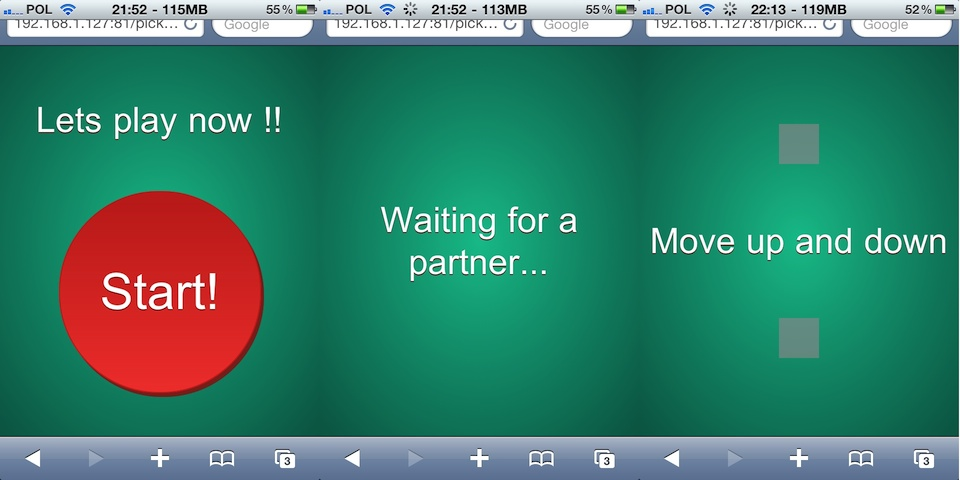
\includegraphics[width=\linewidth]{mobile_screens}
\end{center}
\caption{Zrzut ekranów pokazujący kolejne stany aplikacji od strony klienta}
\label{fig:mobile_screens}
\end{figure}

Po naciśnięciu przycisku Start, klient trafia do kolejki gry, jeśli istnieje możliwość podłączenia się do którejś z trwających gier, to klient zostaje przekierowany do kolejki oczekiwania odpowiedniego serwera. Następnie klient czeka na partnera do gry (co pokazuje drugi widok na rysunku ~\ref{fig:mobile_screens}), lub natychmiastowo zostaje przekierowany do gry i oczom ukazuję się gra której widok został przedstawiony na trzecim zrzucie ekranu. Całym zamysłem gry jest to, że tylko sterowanie grą odbywa się z przeglądarki internetowej klienta, natomiast przebieg gry można obserwować na dużym ekranie tak jak to pokazano na rysunku ~\ref{fig:pong-gameplay}

\begin{figure}
\begin{center}
    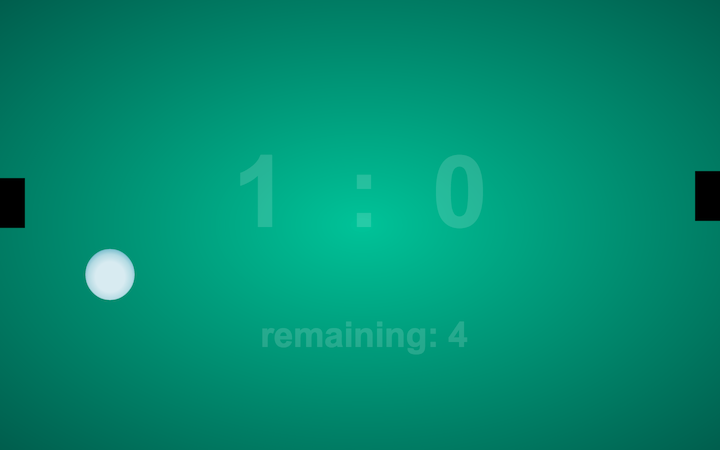
\includegraphics[width=\linewidth]{pong-remote-client-gameplay}
\end{center}
\caption{Zrzut ekranu z trwającej gry}
\label{fig:pong-gameplay}
\end{figure}



\subsection{Aplikacja internetowa zarządzająca infrastrukturą}

Stroną startową aplikacji zarządzającej jest ekran logowania przedstawiony na rysunku ~\ref{fig:managment_login}.

\begin{figure}
\begin{center}
    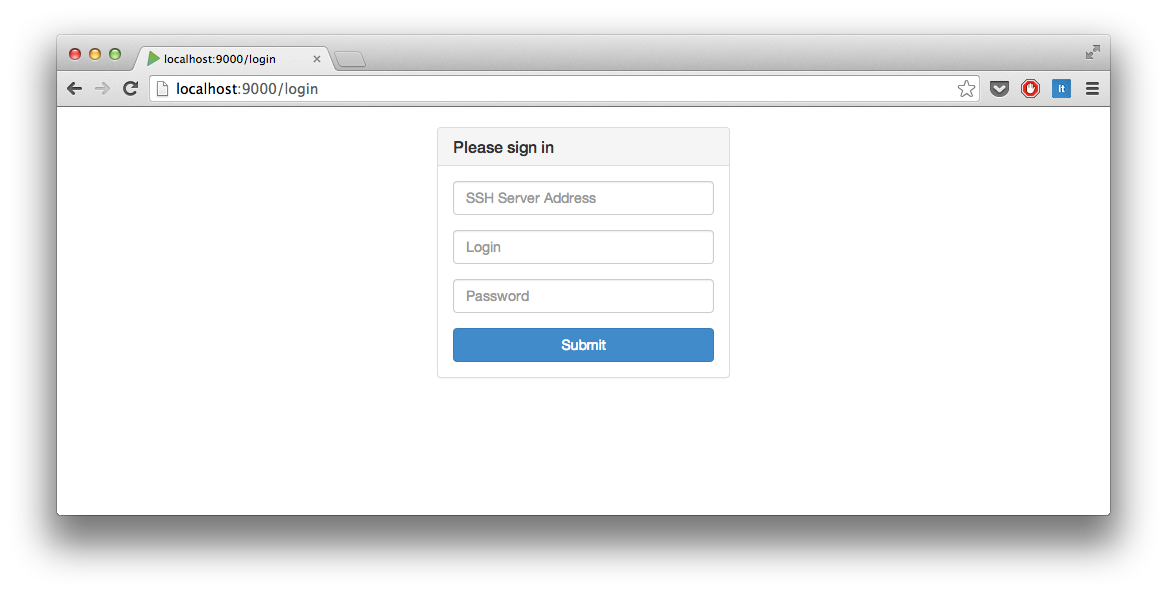
\includegraphics[width=\linewidth]{managment_login}
\end{center}
\caption{Ekran logowania aplikacji zarządzającej infrastrukturą}
\label{fig:managment_login}
\end{figure}

W zakładce Displays istnieje możliwość dodania nowego ekranu po podaniu nazwy, oraz adresu IP wraz z numerem ekranu komputera obsługującego dany wyświetlacz. Po poprawnym dodaniu nowego urządzenia, istnieje możliwość wybrania aplikacji, która będzie wyświetlana na ekranie.

\begin{figure}
\begin{center}
	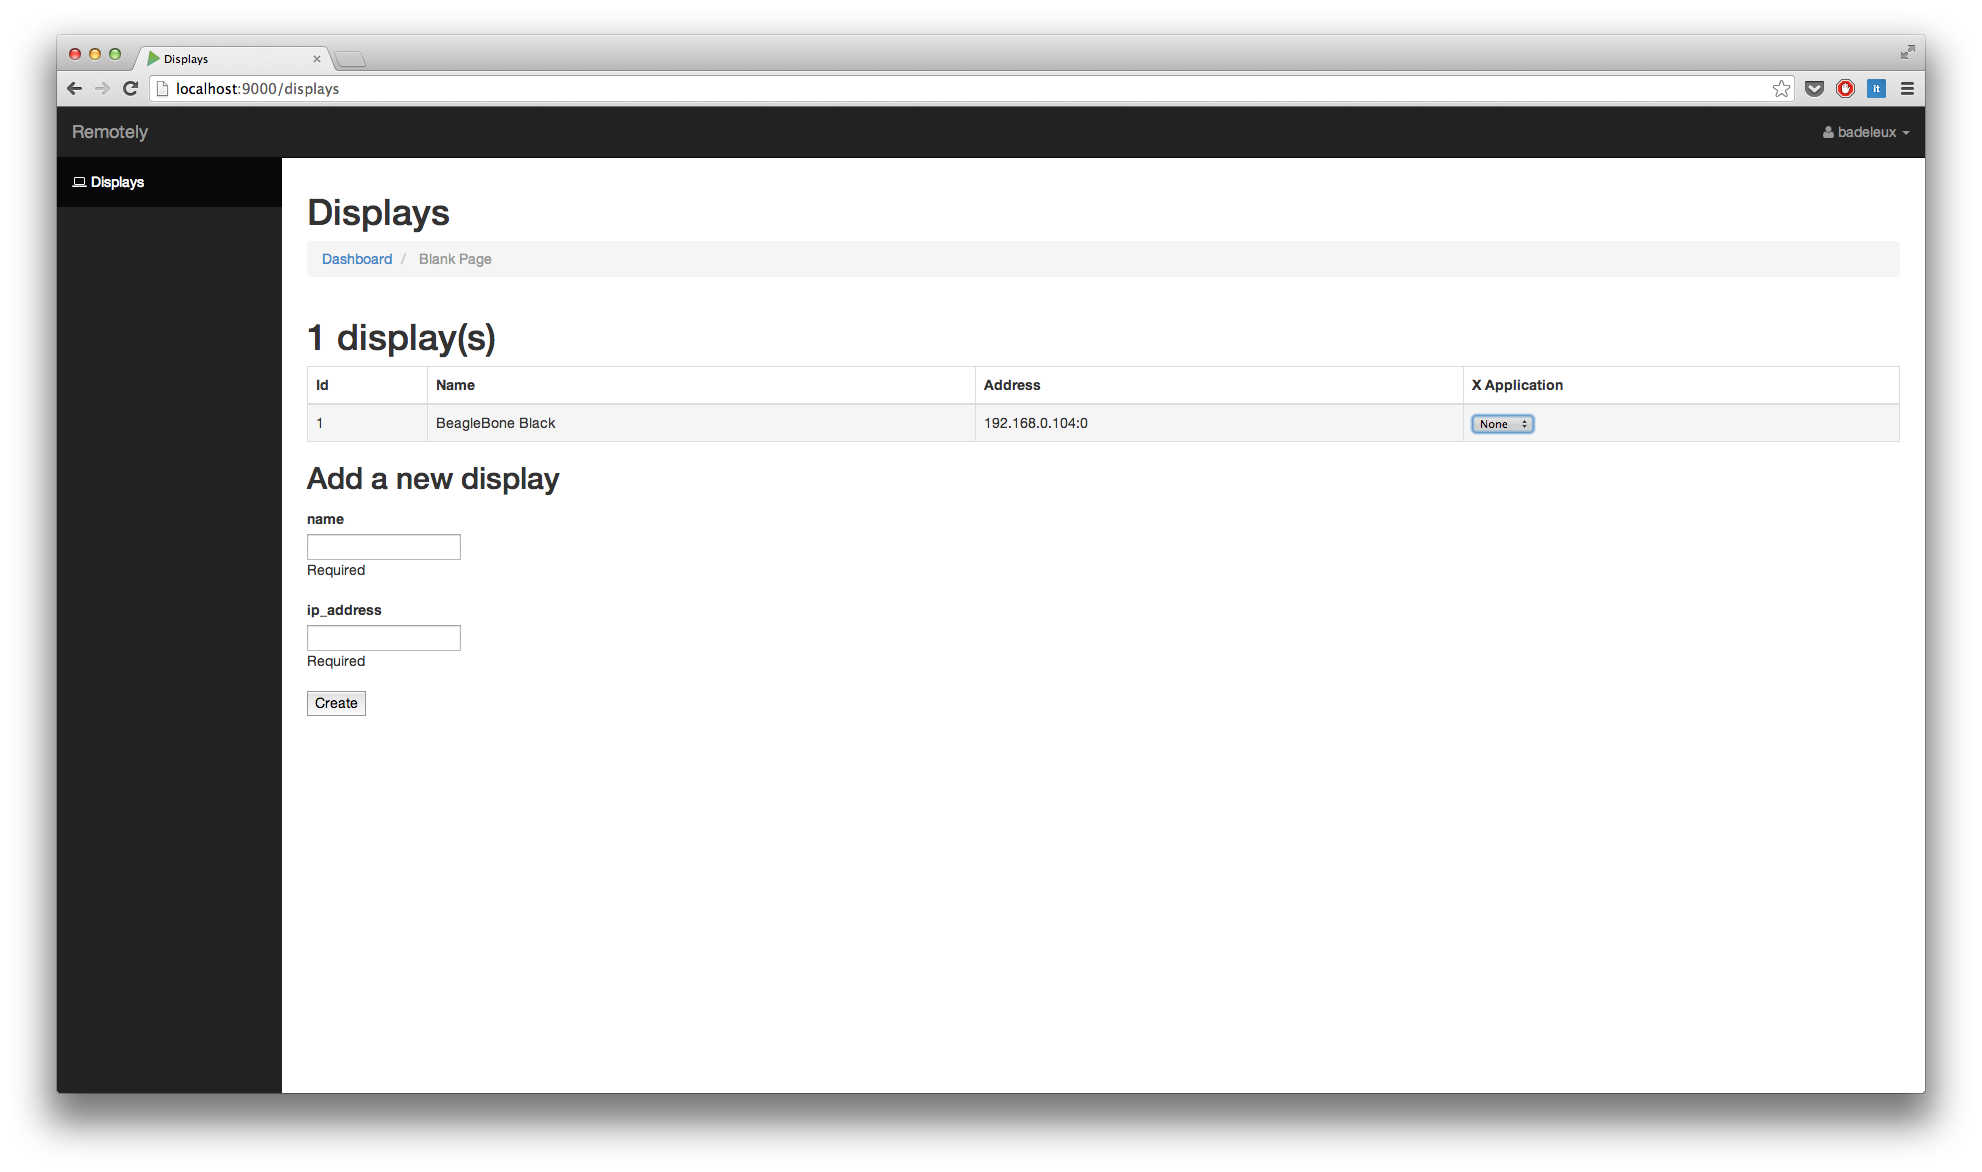
\includegraphics[width=\linewidth]{managment_display}
\end{center}
\caption{Widok zarządzania ekranami}
\label{fig:managment_display}
\end{figure}






\newpage
\section{Architektura systemu}

W ramach pracy dyplomowej stworzone zostaną dwa systemy, które za pomocą tej samej techniki komunikacji zrealizują dwa przykładowe zadania, aby zaprezentować możliwości wykorzystania nowo powstałych standardów. Pierwszym z nich jest pilot umożliwiający porusznie kursorem na ekranie komputera pracującego pod systemem Linux lub MacOSX (opisany szczegółowo w sekcji ~\ref{sec:component-controll-remote-screen}). Drugi system to implementacja gry PONG dla dwóch graczy z możliwością kolejkowania kandydatów do gry.


W załączniku ~\ref{app:network_diagram_app} przedstawiono sieć połączeń pomiędzy fizycznymi komponentami architektury. Rysunek pokazuje możliwość skalowalności systemu.


W niniejszej sekcji zostanie przedstawiona architektura systemu w postaci diagramu komponentów oraz interakcji pomiędzy nimi.

\subsection{Pilot do sterowania zdalnym monitorem}

System pilota do sterowania zdalnym monitorem złożony jest z trzech części:

\begin{enumerate}
  \item \textbf{Klienta webowego} w postaci strony internetowej uruchamianej na w przeglądarce internetowej na urządzeniu mobilnym użytkownika końcowego. Jego celem jest:
  \begin{enumerate}
    \item Podłączenie się do serwera za pomocą Web Socket, utrzymywanie połączenia w przeglądarce internetowej.
    \item Przechwytywania gestów wykonywanych na ekranie urządzenia mobilnego oraz translację współrzędnych punktu ich na absolutną, procentową pozycję kursora na płaszczyźnie dwuwymiarowej \( x, y \in \langle0, 1\rangle \).
    \item Przesyłania danych do serwera w trybie ciągłym przy każdej zmianie pozycji kursora przez przesunięcie palca na ekranie telefonu.
  \end{enumerate}
  
 \item \textbf{Serwera} obsługującego protokół Web Socket, który ma za zadanie obsługę połączeń klientów webowych oraz przekazanie danych do programu sterująego kursorem. Serwer łączy się do programu sterującego kursorem przez standardowe gniazdo systemu operacyjnego.
 
 \item \textbf{Programu sterującego kursorem}, który wystawia standardowe gniazdo systemu operacyjnego, przyjmuje dane od serwera, przetwarza je oraz steruje kursorem myszy na ekranie.
\end{enumerate}

\subsubsection{Diagram komponentów}

TODO: Kamil Badyla
insert as a image

\subsubsection{Diagram interackji}

TODO: Kamil Badyla
insert as a image

\subsection{Gra PONG wyświetlana na zdalnym monitorze}

System gry PONG dla dwóch graczy z możliwością kolejkowania chętnych złożony jest z trzech części:

\begin{enumerate}
  \item \textbf{Klienta webowego} w postaci strony internetowej uruchamianej na w przeglądarce internetowej na urządzeniu mobilnym użytkownika końcowego. Podobnie, jak w przypadku systemu pilota do sterowania zdalnym monitorem, klient ma za zadanie zapewnić komunikację, przechwytywać gesty wykonane na urządzeniu mobilnym oraz wyświetlać komunikaty i przyciski w zależności od stanu gry.
  \item \textbf{Serwera} obsługującego protokół Web Socket, który ma za zadanie obsługę połączeń klientów webowych, kolejkowanie ich zgłoszeń do gry, oraz uruchomienie gry na kliencie wyświetlającego grę. Serwer komunikuje się z klientem wyświetlającym grę za pomocą Web Socket, jako, że jest napisany jako aplikacja uruchamiana w przeglądarce internetowej.
  \item \textbf{Klient wyświetlający grę} - aplikacja stworzona jako strona internetowa uruchamiana w przeglądarce na ekranie LED. Wyświetla planszę gry w trakcie jej trwania, lub komunikaty zachęcające do podjęcia rozgrywki w trakcie, gdy nie trwa rozgrywka. Na ekranie można wyświetlać potencjalne reklamy.
\end{enumerate}



\newpage
\section{Implementacja}

\subsection{Klient webowy}
\label{subsub:impl-webclient}

Klient webowy został zaimplementowany w obu aplikacjach (pilota do sterowania zdalnym monitorem oraz grze PONG) jako statyczna strona internetowa, której kod JavaScript przechowany jest w Web Storage (podsekcja \ref{subsub:webstorage}) za pomocą basket.js (podsekcja \ref{subsub:tools-basketjs}). Komunikacja z serwerem została zrealizowana przy użyciu biblioteki Socket.io (podsekcja \ref{subsub:socketio}), odbywa się ona za pomocą protokołu Web Sockets (podsekcja \ref{subsub:websockets}) lub, w przypadku braku obsługi standardu przez przeglądarkę internetową, z jedną ze wspieranych metod przez bibliotekę Socket.io z modelu Comet (podsekcja \ref{sub:communication-methods}). W aplikacjach wykrywane są dotknięcia ekranu urządzenia mobilnego (sekcja \ref{sub:touch-detection}) przy użyciu biblioteki jQuery Mobile (podsekcja \ref{subsub:tool-jquery-mobile}).

\subsubsection{Reprezentacja kursora na płaszczyźnie}
\label{subsub:cursor-representation}

Kursor jest reprezentowany za pomocą punktu \(C(x_{c}, y_{c})\) o nieujemnych, całkowitych współrzędnych \emph{cursor coordinate} oznaczających jego pozycję od punktu \(P(0, 0)\) umieszczonego w lewym, górnym rogu ekranu, a wektor jest skierowany ku punktowi w prawym dolnym rogu ekranu.

\begin{figure}[h!]
  \centering
    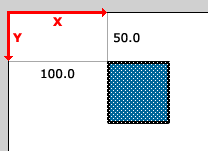
\includegraphics{wyznaczanie-pozycji-kursora}
  \caption{Sposób wyznaczania pozycji kursora myszy.}
\end{figure}

Uwzględniając różne proporcje \(p = \frac{szerokosc}{wysokosc}\) ekranu, na którym pojawia się zdalnie sterowany kursor oraz proporcje powierzchni ekranu urządzenia mobilnego, w implementacji pilota użyta została reprezentacja procentowa punktu na ekranie.

Pozycja kursora reprezentowana jest przez punkt \(P(x, y)\) na dwuwymiarowej płaszczyźnie w zakresie \( x\in \langle0, 1\rangle \), gdzie \(x = \frac{x_{c}}{w_{x}}\), \(y = \frac{x_{c}}{w_{y}}\), a \(w_{x}\) oraz \(w_{y}\) oznaczają kolejno szerokość i wysokość ekranu.

Wyznaczanie pozycji uwzględnia również zmianę orientacji (poziomej lub pionowej), szerokości i wysokości rzutni okna przeglądarki wyświetlanej na urządzeniu mobilnym.

\lstset{language=JavaScript}
\begin{lstlisting}
this.run = function() {
	
	var this = that
	this.windowX = 0
	this.windowY = 0
	
	$(document).on('vmousemove', function(e) {
		e.preventDefault(); // prevent scroll
		
		var x = e.pageX / that.windowX
		var y = e.pageY / that.windowY
		
		console.log(x, y) // wypisz punkty
	})
	
	var indicateWindowSize = function() {
		that.windowX = $(window).width()
		that.windowY = $(window).height()
	}
	
	// register window size changes listeners
	$(window).on('resize orientationchange', function() {
		indicateWindowSize()
	})
	indicateWindowSize()
}
\end{lstlisting}

\subsubsection{Pilot do sterowania zdalnym monitorem}

Logika aplikacji pilota jest trywialna. Przechwytuje punty zestyku użytkownika z urządzeniem mobilnym, przekształca reprezentację współrzędnych (podsekcja \ref{subsub:cursor-representation}) i wysyła do je do serwera w postaci współrzędnych x, y za pomocą metody \lstinline{emit()} biblioteki socket.io (podsekcja \ref{subsub:socketio}) wiadomością o temacie \emph{mouseMoveToPercent}:

\lstset{language=JavaScript}
\begin{lstlisting}
this.run = function() {
	// init socket connection
	that.socket = socketConnect(that.socket, that.serverAddress);
	
	that.socket.emit('connectToRemote', {
		host: that.serverRemoteHost,
		port: that.serverRemotePort
	})
	
	// register listeners
	$(window).on('resize orientationchange', function() {
		indicateWindowSize()
	})
	indicateWindowSize()
	
	$(document).on('vmousemove', function(e) {
		e.preventDefault(); // prevent scroll
		
		var x = e.pageX / that.windowX
		var y = e.pageY / that.windowY
		
		if(that.x == null || that.y == null || Math.abs(that.x - x) > that.minDelta || Math.abs(that.y - y) > that.minDelta) {
			that.x = x
			that.y = y
			
			var data = {
				x: x,
				y: y
			}
			
			that.socket.emit('mouseMoveToPercent', data)
		}
	})
}
\end{lstlisting}

Aplikacja posiada również zapisy konfiguracji (nazwa hosta oraz port) połączenia do serwera programu generującego zdarzenia urządzeń wejścia (podsekcja \ref{sub:impl-displayclient-events-dispatcher}), do którego ma być przekazywana pozycja, którą wysyła wiadomością o temacie \emph{connectToRemote}. Przykładowa konfiguracja\footnote{Pełen opis instalacji w podsekcji \ref{subsub:setup-server-nodejs}}:

\lstset{language=HTML}
\begin{lstlisting}
<body data-server="192.168.1.127:8080" data-server-remote-host="192.168.1.127" data-server-remote-port="8081">
</body>
\end{lstlisting}

Interfejs wyjściowy aplikacji obejmuje dwa komunikaty: \emph{mouseMoveToPercent} i \emph{connectToRemote}.

\begin{description}
	\item[mouseMoveToPercent] \hfill \\
	Komunikat wysyłany do serwera, informujący o pozycji kursora.
	\begin{enumerate}
		\item x (float)
		\item y (float)
	\end{enumerate}
\end{description}

\begin{description}
	\item[connectToRemote] \hfill \\
	Komunikat wysyłany do serwera, informujący o połączeniu do serwera programu generującego zdarzenia urządzeń wejścia.
	\begin{enumerate}
		\item host (string)
		\item port (float)
	\end{enumerate}
\end{description}

Interfejs wejściowy aplikacji:

Brak.

\subsubsection{Pilot gry PONG wyświetlanej na zdalnym monitorze}

Pilot do sterowania grą PONG wyświetlaną na zdalnym monitorze umożliwia zgłoszenie chęci uczestnictwa w grze oraz sterowanie paletką. Na ekranie startowym użytkownik widzi przycisk, dzięki któremu może zgłosić chęć uczestnictwa w grze, następnie pilot wyświetla komunikaty, aż wreszcie umożliwia sterowanie paletką. Aplikacja jest napisana w jQuery oraz ostylowana arkuszem napisanym w CSS 3.

Interfejs wyjściowy aplikacji obejmuje jeden komunikat: \emph{paddleMove}.

\begin{description}
	\item[paddleMove] \hfill \\
	Komunikat informujący serwer o zmianie położenia punktu zestyku użytkownika z ekranem:
	\begin{enumerate}
		\item positionX (float)
		\item positionY (float)
	\end{enumerate}
\end{description}

Interfejs wejściowy aplikacji (komunikaty wysyłane przez serwer do klienta) obejmuje cztery komunikaty: \emph{signalCurrentServerState}, \emph{signalWaitingForPartner}, \emph{welcome} i \emph{gameOver}.

\begin{description}
	\item[signalCurrentServerState] \hfill \\
	Komunikat informujący o stanie gry oraz kolejki. Odbierany jest za każdym razem, gdy zmienia się stan gry: ilość użytkowników oczekujących na grę, włączenie gry. Na podstawie otrzymanych danych wyświetla się komunikat, który w kolejce jest użytkownik.
	\begin{enumerate}
		\item count (int) liczba użytkowników oczekujących w kolejce do gry
		\item isGame (boolean) informacja, czy jest rozgrywana gra, czy nie
	\end{enumerate}
\end{description}

\begin{description}
	\item[signalWaitingForPartner] \hfill \\
	Komunikat oznaczający, że klient został przyjęty do kolejki oczekujących graczy i oczekuje na partnera do gry.
\end{description}

\begin{description}
	\item[welcome] \hfill \\
	Komunikat oznaczający, że klient rozpoczyna grę.
\end{description}

\begin{description}
	\item[gameOver] \hfill \\
	Komunikat wysyłany przez serwer informujący o zakończeniu gry. Na podstawie otrzymanych danych wyświetla się informacja, czy klient przegrał, czy wygrał.
	\begin{enumerate}
		\item score (int) wynik klienta
		\item scoreEnemy (int) wynik przeciwnika
	\end{enumerate}
\end{description}


\section{Serwer}

Klient webowy uruchamiany w przeglądarce internetowej na urzadzeniu mobilbym użytkownika końcowego łączy się z serwerem przez sieć\footnote{Diagram komponentów w dodatku \ref{app:netwo}}, który odpowiada za poprawne działanie systemu. Korzystając z nowych możliwości przeglądarek internetwoych zaimplementowano dwustronną komunikację (ang. \emph{full duplex communication}) przy uzyciu mechanizmu \emph{Web Sockets}\cite{websockets-rfc} opisaną w podsekcji \ref{subsub:websockets}. Dla urządzeń nie wspierających Web Sockets, przy użyciu biblioteki \emph{Socket.io} (opisanej w podsekcji \ref{subsub:socketio}) dostępne są inne mechanizmy (przegląd w podsekcji \ref{sub:communication}) dwustronnej komunikacji nie wykazujące tak szybkiego działania.

\subsection{Komunikacja między klientem webowym, a serwerem}
\label{sub:communication-methods}

W obu aplikacjach, zarówno grze PONG, jak i pilocie sterującym zdalnym monitorem komunikacja między rozproszonym systemem jest oparta o asynchroniczną wymianę komunikatów (ang. \emph{Asynchronous Message-oriented middleware - MOM})\cite{message-oriented-middleware}.

Dodatkowo przeprowadzano dywagację na temat skalowania stworzonego systemu opisaną w podsekcji \ref{subsub:scalability}. W obliczu skalowalności klienci łączą się do centralnego serwera, który rozdysponuje ruch sieciowy pomiędzy dostępne serwery (ang. \emph{nodes}) obsługujących żądania. W kontekście rozproszenia systemu, architektura MOM polega na asynchronicznem modelu wymiany komunikatów, w przeciwieństwie do modelu żądanie-odpowiedź (\emph{request-response model}). W asynchronicznych systemach kolejki komunikatów pełnią rolę tymczasowego bufora, kiedy odbiorca wiadomości jest zajęty lub niepodłączony do sieci. W dodatku istnieje możliwość stworzenia kolejek trwałych (ang. \emph{persistent queues}), w których wiadomości są zapisywane w pamięci trwałej (np. na dysku) zachowania ich kopii, dzięki czemu nadawca i odbiorca wiadomości nie musi być dostępny w sieci w tym samym czasie - mechanizm ten nazywany jest asynchroniczną dostawa (ang. \emph{asynchronous delivery}). Oznacza to, że gdy odbiorca wiadomości jest niedostępny, wysyłający wiadomości może pracować, a wiadomości zostaną odłożone w kolejce celem późniejszej dostawy, kiedy odbiorca będzie dostępny.

\begin{figure}[H]
  \caption[Model asynchronicznej interakcji w systemach opartych o wymianę komunikatów]{Model asynchronicznej interakcji w systemach opartych o wymianę komunikatów}
  \centering
    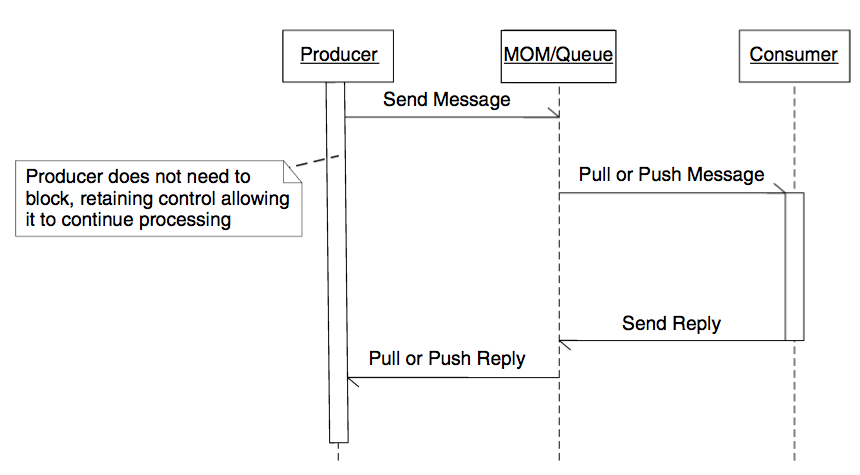
\includegraphics[width=\linewidth]{mom-flow.png} \\
    Diagram UML przepływu przedstawiający model producenta i konsumenta wiadomości połączonego przez system kolejek, źródło\cite{message-oriented-middleware}
\end{figure}

\begin{figure}[H]
  \caption[Schemat działania kolejki w systemach opartych o wymianę komunikatów]{Schemat działania kolejki w systemach opartych o wymianę komunikatów}
  \centering
    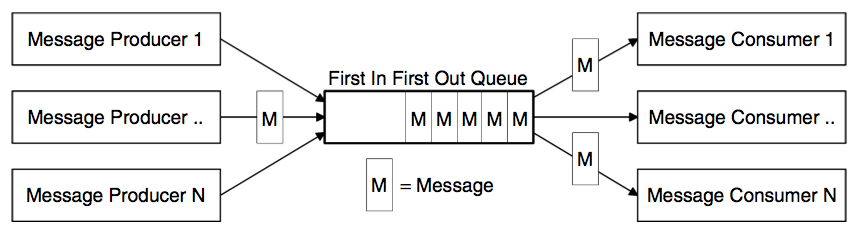
\includegraphics[width=\linewidth]{mom-queue.png} \\
    Diagram przedstawiający model producenta i konsumenta wiadomości połączonego przez system kolejek FIFO, źródło\cite{message-oriented-middleware}
\end{figure}

\subsection{Mechanizmy komunikacji}
\label{sub:communication-methods}

Protokół HTTP\footnote{Hypertext Transfer Protocol} przewiduje komunikację inicjowaną przez klienta do serwera\cite{http-rfc}. Klient wysyła żądanie (ang. \emph{request}) złożoną z nagłówków (ang. \emph{headers}) oraz treści (ang. \emph{body} lub \emph{content}), natomiast serwer zwraca odpowiedź również w postaci nagłówków oraz treści. Każde żądanie jest bezstanowe, swego rodzaju transakcją, to znaczy, że nie zależy od poprzedniego, ani kolejnego. Aby zapewnić transakcyjność stosuje się mechanizmy podtrzymania sesji użytkownika za pomocą przesyłania w nagłówkach ciasteczek zawierający unikatowy identyfikator sesji znany zarówno po stronie klienta, jak i serwera - tym sposobem serwer jest w stanie zidentyfikować następujące po sobie bezstanowe żądania. Istotnym minusem w kontekście prowadzenia komunikacji w protokole HTTP jest to, że serwer nie może zainicjować wysłania danych do przeglądarki, bowiem połączenie jest zamykane zaraz po odesłaniu odpowiedzi. Komunikacja jest jednostronna (ang. \emph{half-duplex communication}).

Przykładowe zapytanie:
\lstset{language=Octave}
\begin{lstlisting}
GET /path/file.html HTTP/1.1\r\n
Host: www.host1.com:80\r\n
\r\n
\end{lstlisting}

Przykładowa odpowiedź:
\lstset{language=Octave}
\begin{lstlisting}
HTTP/1.1 200 OK\r\n
Date: Fri, 31 Dec 1999 23:59:59 GMT\r\n
Content-Type: text/plain\r\n
Transfer-Encoding: chunked\r\n
\r\n \#\# oznacza pusta linie
TUTAJ TRESC
\end{lstlisting}

Aby zapewnić komunikację dwustronną (ang. \emph{full-duplex communication}) (tj. aby serwer mógł wysyłać wiadomości do przeglądarki internetowej w trybie \emph{server push}) stosuje się wiele zabiegów, znanych pod pojęciem komety (ang. \emph{Comet}), których przegląd jest zamieszczony poniżej. Inne znane nazwy tożsame z Comet: \emph{Ajax Push},\footnote{ICEfaces.org [Data dostępu: 27 grudnia 2013]} \emph{Reverse Ajax}\footnote{Crane, Dave; McCarthy, Phil (Lipiec 2008). \emph{Comet and Reverse Ajax: The Next Generation Ajax 2.0}. Apress. ISBN 1-59059-998-5}, \emph{Two-way-web}, \emph{HTTP Streaming}, \footnote{Mahemoff, Michael (Czerwiec 2006). \emph{Web Remoting}. Ajax Design Patterns. O'Reilly Media. s. 19; 85. ISBN 0-596-10180-5}, oraz \emph{HTTP server push}\footnote{Double, Chris (2005-11-05). \emph{"More on Ajax and server push". Different ways of doing server push.}}.

\subsubsection{Komunikacja HTTP persistent connection}
\label{subsub:http-persistent-connection}

Protokół HTTP w wersji 1.0 umożliwia tworzenie stałych połączeń (ang. \emph{persistent connection}) przez przesłanie nagłówka Connection: Keep-Alive, serwer w ramach odpowiedzi odsyła ten sam nagłówek, a od wersji protokołu 1.1 Keep-Alive jest uznawane za domyślne i nie jest konieczne wysłanie nagłówka. Otwarte połączenie przez przeglądarkę internetową nie zamyka go po tuż otrzymaniu odpowiedzi od serwera, a podtrzymuje je mogąc wysłać w ramach niego kilka żądań. Optymalizacja ma na celu zmniejszenia czasu wykonywania żądań o czas otwarcia połączenia po stronie przeglądarki internetowej oraz serwera. Korzyści jest znacznie więcej:

\begin{itemize}
	\item mniejsze zużycie procesora i pamięci operacyjnej,
	\item możliwość wykonania kilku żądań i odpowiedzi jedno po drugim (ang. \emph{pipelining}),
	\item zmniejszenie ruchu sieci (mniej połączeń TCP),
	\item zmniejszone opóźnienie (ang. \emph{latency}) związane z nawiązaniem połączenia z odległym hostem,
	\item w przypadku żądań HTTPS\footnote{Secured HTTP, połączenie podpisane certyfikatem SSL} zmniejsza się liczba obiegów sieci (ang. \emph{network round-trips}) celem wymiany kluczy publicznych oraz certyfikatu.
\end{itemize}

\begin{figure}[H]
  \caption[HTTP Persistent Connection]{HTTP Persistent Connection}
  \centering
    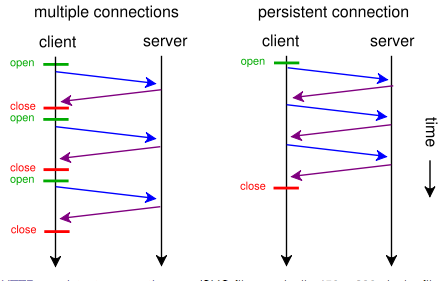
\includegraphics[scale=0.75]{http-persistent-connection.png} \\
    Rysunek przedstawia wysyłanie kolejnych żądań HTTP w ramach osobnych połączeń (domyślnie HTTP 1.0, po lewej stronie) oraz w ramach jednego połączenia (persistent connection, po prawej).
\end{figure}

\subsubsection{HTTP Server Push, Pushlet, JSONP Pooling oraz Script Tag long pooling, Hidden IFRAME}

Korzystając z możliwości użycia \emph{persistent connections} (opisanego w podsekcji \ref{subsub:http-persistent-connection}) powstały mechanizmy umożliwiające komunikację ze strony od serwera do klienta w trybie push:

\begin{description}
  \item[HTTP Server Push] \hfill \\
  Mechanizm polega na tym, że klient inicjuje żądanie, serwer natomiast podtrzymuje je w trybie zawieszonym (nie odsyła odpowiedzi, połączenie pozostaje otwarte), a gdy wystąpi zdarzenie, może zostać ono wysłane do klienta w trybie natychmiastowym. Jeżeli zachodzi zdarzenie, a klient nie jest podłączony, może zostać dodane do kolejki do wysłania przy następnym żądaniu klienta. Po otrzymaniu odpowiedzi i zerwaniu połączenia klient inicjuje nowe żądanie powtarzając cały proces w pętli. Zwalnia to z konieczności periodycznego sprawdzania, czy zaszły jakieś zdarzenia na serwerze poprzez odpytywania serwera (ang. \emph{pooling}).

  \begin{figure}[H]
    \caption[Zasada działania HTTP Server Push]{Zasada działania HTTP Server Push}
    \centering
      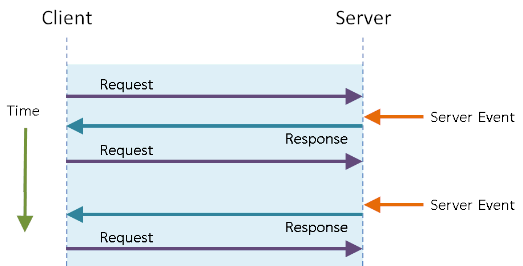
\includegraphics[scale=0.75]{http-server-push.png}
  \end{figure}

  \begin{figure}[H]
    \caption[Porównanie HTTP Pooling oraz HTTP Long Pooling]{Porównanie HTTP Pooling oraz HTTP Long Pooling}
    \centering
      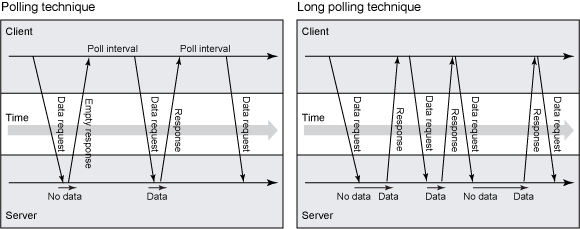
\includegraphics[scale=0.65]{http-pooling-vs-longpooling.jpg}
  \end{figure}

  \item[Pushlet] \hfill \\
  Podejście polegające na podtrzymaniu zainicjowanego połączenia przez klienta w trybie zawieszonym w stanie ciągłego ładowania odpowiedzi (serwer nigdy nie zamyka połączenia). Umożliwia to ciągłe dostarczanie treści do odpowiedzi, która jest interpretowana przez przeglądarkę, np w postaci kodu JavaScript osiągając w ten sposób możliwość wysyłania odpowiedzi z serwera do klienta. W ten sposób po stronie klienta nie jest konieczne uruchomienie appletu Java lub kodu Flash, które dostarczając opcję otwarcia połączenia, ale wymagają zezwolenia od użytkownika.

  \item[XHR Pooling] \hfill \\
  Możliwe jest wykorzystanie obiektu \lstinline{XMLHttpRequest} (\emph{XHR})\cite{xhr-rfc} wykorzystywane w aplikacjach AJAX (ang. \emph{Asynchronous JavaScript and XML}), który umożliwia asynchroniczne odbieranie framgmentow treści strony bez konieczności odświeżenia całej jej zawartości (ponowienia żądania i odpowiedzi). Dane mogą być odbierane w dowolnym formacie, co umożliwia wykorzystanie mechanizmu Comet.\\

  W 1995 roku przeglądarka Netscape Navigator wprowadziła mechanizm który umożliwił serwerowi odświeżanie zawartości obrazka lub kodu HTML wysyłając odpowiedź jako wieloczęściową (ang. \emph{multipart response}) oznaczając ją nagłówkiem

\lstinline{Content-type: multipart/x-mixed-replace}\cite{xhr-rfc}

  Po stornie serwera, każde zdarzenie, które ma być wysłane do klienta jest kolejną częścią odpowiedzi HTTP, odbierane po stronie klienta i interpretowane w wywoływanej funkcji wskazanej jako callback \lstinline{onreadystatechange} wykonywanej za każdym razem, gdy pojawią się nowe dane. Umożliwia to dosyłanie dowolnych porcji danych.

  \item[Hidden IFRAME] \hfill \\
  Technika znana również pod nazwą \emph{forever frame}, polegająca na umieszczeniu w kodzie strony www ukrytej ramki (umożliwiającej wstawienie dokument HTML pochodzący z innej strony internetowej) wykorzystującej mechanizm Pushlet. Gdy wystąpi zdarzenie na serwerze, może ono zostać wysłane jako treść odpowiedzi w postaci tagu HTML
  \lstinline{<script>}
  wypełnionego treścią wykonywalnego kodu JavaScript, który jest natychmiastowo interpretowany przez przeglądarkę. Dokument HTML przyrasta o nowe tagi \lstinline{<script>}. Podstawową zaletą tego rozwiązania jest to, że jest obsługiwane przez każdą przeglądarkę.

  \item[Script Tag long pooling] \hfill \\
  Wszystkie wcześniej wymienione sposoby komunikacji w trybie push od strony serwera wykorzystujące protokół HTTP nie są zdolne do wykonania żądania inicjującego przez klienta poza domenę ze względu na \emph{Same Origin Policy}, bowiem nie można wykonywać połączeń XHR poza domenę\footnote{SLDs - second-level domains} oraz przechwytywać zdarzeń JavaScript z ramki IFRAME z innej domeny. Istnieje sposób na wczytywanie danych spoza domeny za pomocą wczytywania kodu javascript tagiem \lstinline{<script>}, który może wskazywać dowolny adres url wykorzystując technikę Pushlet oraz doładowywać fragmentu kodu JavaScript natychmiastowo wykonywane po stronie przeglądarki.
  
  \item[JSONP Pooling] \hfill \\
  Oparta na technice \emph{Script Tag long pooling} polegająca na doładowywaniu kodu JavaScript zawierającego dane w postaci JSON\footnote{JSON - JavaScript Object Notation} przekazywane jako argument wskazanej wcześniej funkcji w postaci obiektu JavaScript.
  
  Przykład wywołania JSONP Pooling:
\lstset{language=HTML}
\begin{lstlisting}
  <script type="application/javascript"
     src="http://example.com/?functionName=parseResponse">
  </script>
\end{lstlisting}
  
  Jako argument zapytania zostanie wysłana nazwa funkcji, którą serwer umieszcza w odpowiedzi. Jako treść kodu JavaScript wywołuje wskazaną funkcję. Przykładowa odpowiedź serwera:

\lstset{language=JavaScript}
\begin{lstlisting}
   parseResponse({"Name": "Foo", "Id": 1234, "Rank": 7});
\end{lstlisting}

\end{description}

\subsubsection{Metody oparte o wykorzystanie Flash i Java Applets}

Wykorzystując możliwości osadzanych niewidocznych (lub małych, 1x1 pikseli\footnote{one-pixel element}) elementów Flash oraz appletów Java zapewnia się mechanizmy otwierające połączenie TCP bezpośrednio z tych elementów, a komunikacja z przeglądarką internetową odbywa się za pomocą wywoływania funkcji JavaScript z przekazywanymi danymi. Niestety, Flash oraz applety Java nie są wspierane przez przeglądarki na urządzeniach mobilnych, a każda interakcja często jest poprzedzona zgodą klienta.

\subsubsection{Web Sockets}
\label{subsub:websockets}

Opisane metody w sekcji \ref{sub:communication-methods} nie zapewniają komunikacji dwukierunkowej (ang. \emph{full-duplex} lub \emph{bi-directional communication}) za pomocą jednego połączenia TCP. Wychodząc na przeciw oczekiwaniom twórców witryn www czasu rzeczywistego wprowadzony został mechanizm \emph{Web Sockets} ustandaryzowany przez IETF\footnote{Internet Engineering Task Force} w dokumencie RFC-6455\cite{websockets-rfc} umożliwiający nawiązanie połączenia TCP wprost z przeglądarki internetowej. W chwili obecnej większość przeglądarek internetowych wspiera standard Web Sockets\cite{caniuse-websockets}, w tym przeglądarki na urządzeniach mobilnych.

\begin{figure}[H]
  \caption[Zasada działania protokołu Web Sockets]{Zasada działania protokołu Web Sockets}
  \centering
    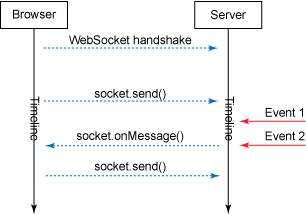
\includegraphics[scale=0.75]{websockets-flow.jpg}
\end{figure}

Protokół Web Sockets został zaprojektowany dla przeglądarek internetowych, natomiast może być użyty w jakiejkolwiek aplikacji. Opiera się na protokole HTTP, ale tylko do czasu przełączenia za pomocą \emph{Upgrade Request} na właściwą wymianę danych, by przystąpić do etapu \emph{handshake}. Aby ustanowić połączenie w protokole Web Sockets, klient wysyła żądanie w protokole HTTP:

\lstset{language=Octave}
\begin{lstlisting}
GET /chat HTTP/1.1
Host: server.example.com
Upgrade: websocket
Connection: Upgrade
Sec-WebSocket-Key: dGhlIHNhbXBsZSBub25jZQ==
Origin: http://example.com
Sec-WebSocket-Protocol: chat, superchat
Sec-WebSocket-Version: 13
\end{lstlisting}

Klient wysyła nagłówek \lstinline{Sec-WebSocket-Key} o wartości będącej wartością losową zakodowaną jako base64\footnote{Jeden ze sposobów kodowania ciągów bajtów}.

Serwer wysyła odpowiedź \emph{101 Switching Protocols}:

\lstset{language=Octave}
\begin{lstlisting}
HTTP/1.1 101 Switching Protocols
Upgrade: websocket
Connection: Upgrade
Sec-WebSocket-Accept: s3pPLMBiTxaQ9kYGzzhZRbK+xOo=
Sec-WebSocket-Protocol: chat
\end{lstlisting}

W odpowiedzi na nagłówek \lstinline{Sec-WebSocket-Key} serwer odsyła w odpowiedzi nagłówek \lstinline{Sec-WebSocket-Accept} o wartości będącą równą:

\vspace*{1\baselineskip}
\lstinline{base64(sha1( klucz ))}
\vspace*{1\baselineskip}

Gdzie klucz to sklejenie ciągu znaków pochodzących z wartości \lstinline{Sec-WebSocket-Key} oraz stałej, ustalonej wartości \lstinline{258EAFA5-E914-47DA-95CA-C5AB0DC85B11}.

Od tego momentu rozpoczyna się transmisja w protokole Web Socekts, grze przesyłane są ramki w trybie full-duplex:

\begin{figure}[H]
  \caption[Ramka protokołu Web Sockets]{Ramka protokołu Web Sockets}
  \centering
    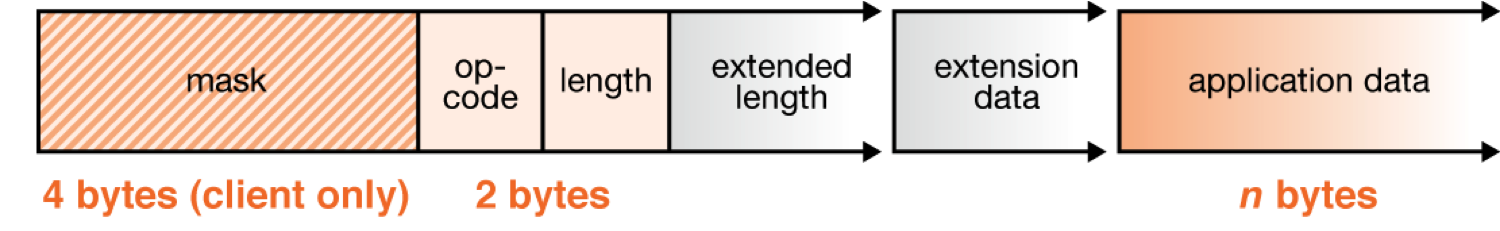
\includegraphics[scale=0.65]{WebSocketFrame.png}
\end{figure}

\subsection{Wykorzystana technologia}

Część serwerowa infrastruktury została napisana w środowisku \emph{Node.js}, stworzonego przez Ryana Dahla w 2009 roku. Node.js używa składni skryptowego\footnote{Kod języków skryptowych wykonywany jest wewnątrz jakiejś aplikacji/środowiska w odróżnieniu od programów napisanych w językach nieskryptowych, które kompilują się i stanowią aplikację} języka JavaScript znanego z tworzenia dynamicznych elementów stron internetowych. Kod JavaScript, choć wykonuje się w ramach przeglądarki internetowej, w Node.js uruchamiany jest po stronie serwera. Technologia umożliwia dużą przepustowość zapewniając nieblokujące operacje wejścia/wyjścia (ang. \emph{non-blocking I/O}) i pętli zdarzeń w pojedynczym wątku \emph{single-threaded event loop}. Podejście to nazywa się programowaniem asynchronicznym (opisanym w podsekcji \ref{subsub:asyncprogramming}).

Wybór platformy obsługującej programowanie asynchroniczne jest jednoznaczny ze względu na specyfikę aplikacji. Większość z nich to oczekiwanie na dane z sieci (ang. \emph{network I/O}). Jeżeli program byłby napisany w modelu synchronicznym, procesor przeznaczałby większość czasu na oczekiwanie na dane z sieci zawieszając (ang. \emph{idle}) jego pracę na funkcjach wejścia/wyjścia. Tymczasem, aby zwiększyć możliwości (uruchomienie tysięcy operacji I/O jednocześnie) korzysta się z asynchronicznego, nieblokującego podejścia pisania aplikacji za pomocą pętli zdarzeń uruchomionej w pojedynczym wątku. Podejście jest odpowiednie do czasu, gdy program nie wykonuje złożonych czasowo operacji, które to mogłyby zawiesić działanie pętli komunikatów uruchomionej w pojedynczym wątku. Większość operacji w stworzonej aplikacji to przekazywanie struktur danych i praca w sieci.

\subsubsection{Synchroniczny i imperatywny model programowania}

W porównaniu do programowania asynchronicznego przedstawione krótko zostanie programowanie imperatywne, będące paradygmatem programowania\cite{programming-paradigms} które opisuje kod programu jako sekwencyjnie wykonywany ciąg instrukcji zmieniający stan programu (rejestrów, pamięci). Takie wyobrażenie przepływu programu jest de facto tożsame z fizyczną realizacją kodu maszynowego na komputerze. W tym modelu przebieg programu możemy zdefiniować jako ciąg następujących po sobie instrukcji\ref{fig:syncprogramming-flow}, dzięki czemu jego przebieg jest przewidywalny, bowiem wykonując bieżącą instrukcję można założyć, ze poprzednia się zakończyła powodzeniem, a jej wyniki są dostępne do użycia. Implikuje to, że wykonywanie każdej operacji jest blokujące\ref{fig:syncprogramming-waiting}. Rozwiązaniem tego problemu jest uruchamianie przebiegu programu w wątkach\ref{fig:syncprogramming-threads} mogących komunikowanie się między sobą lub uruchomienie programu jako nowy proces w systemie operacyjnym\footnote{Te zabiegi powodują narzut czasowy związany z przełączaniem kontekstu pracy procesora w postaci odłożeniem stanu rejestrów, mapy pamięci, rejestrów stosu, FPU itd.}.

\begin{figure}[ht]
\centering
\begin{minipage}[b]{0.45\linewidth}
  \label{fig:syncprogramming-flow}
  \caption[Programowanie synchroniczne - przebieg instrukcji programu w czasie]{Programowanie synchroniczne - przebieg instrukcji programu w czasie}
  \centering
    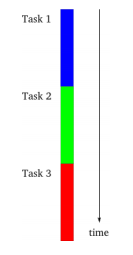
\includegraphics[scale=0.5]{syncprogramming-flow.png}
\end{minipage}

\begin{minipage}[b]{0.45\linewidth}
\label{fig:syncprogramming-threads}
  \caption[Programowanie synchroniczne - wątki]{Programowanie synchroniczne - wątki}
  \centering
    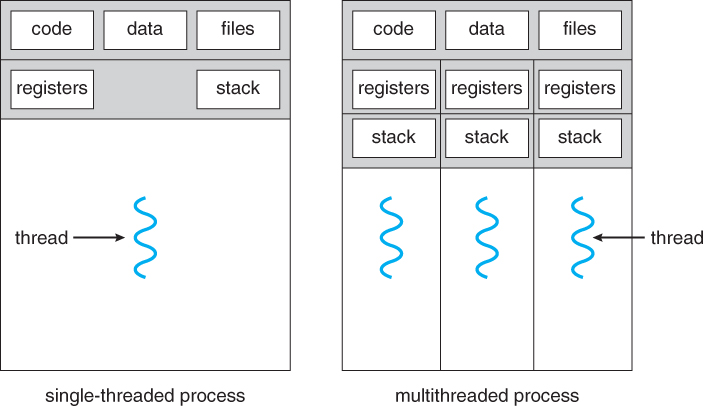
\includegraphics[scale=0.5]{syncprogramming-threads.jpg}
\end{minipage}

\begin{minipage}[b]{0.45\linewidth}
\label{fig:syncprogramming-waiting}
  \caption[Programowanie synchroniczne - operacje blokujące]{Programowanie synchroniczne - operacje blokujące}
  \centering
    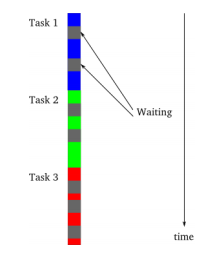
\includegraphics[scale=0.5]{syncprogramming-waiting.png}
\end{minipage}
\end{figure}

\subsubsection{Asynchroniczny model programowania}
\label{subsub:asyncprogramming}

Asynchroniczny model programowania oparty jest na programie uruchomionym w jednym wątku. Znany jest z frameworków graficznych interfejsów użytkownika GUI (na przykład WinApi). W uproszczeniu, budowa programu to nieskończona pętla oraz kolejka operacji odłożona na stos. Z każdym przebiegiem pętla sprawdza w kolejce operacji, czy możliwe są do wykonania jakieś operacje, jeżeli tak, uruchamiane są procedury obsługi (ang. \emph{handlers} lub \emph{callbacks}). Umożliwia to realizację wielu operacji, które oczekują na wyniki bez blokowania pracy całego programu.

\begin{figure}[H]
  \caption[Event loop w asynchronicznym modelu programowania]{Event loop w asynchronicznym modelu programowania}
  \centering
    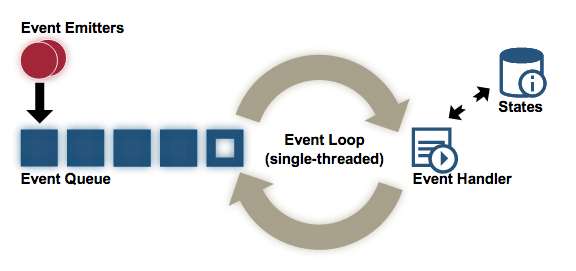
\includegraphics[width=\linewidth]{asyncprogramming-loop.png}
\end{figure}

Realizacja niskopoziomowa to użycie funkcji \lstinline{select()} (zarówno systemów POSIX jak i Windows), deskryptorów \lstinline{/dev/poll}, kqueue, poll i epool. Warta rozpoznania jest biblioteka \emph{libevent}\footnote{\url{http://libevent.org/}}, która zakłada abstrakcję na użyte mechanizmy z punktu widzenia programisty\cite{programming-async-sockets}.

Funkcja \lstinline{select()} przyjmuje za parametry deskryptory oraz maksymalny czas upływu. Zwraca wartość jeżeli a) upłynie zdefiniowany czas lub b) gdy w deskryptorze (reprezentującym plik, urządzenie, gniazdo sieciowe lub strumień danych) zajdą zmiany - będzie dostępny do zapisu lub są dostępne dane do odczytu:

\lstset{language=C}
\begin{lstlisting}
#include <sys/time.h>
#include <sys/types.h>
#include <unistd.h>

int select(int numfds, fd_set *readfds, fd_set *writefds,
           fd_set *exceptfds, struct timeval *timeout);
\end{lstlisting}

W przeciwieństwie do synchronicznego modelu w programowaniu imperatywnym, model asynchroniczny wypada korzystniej, gdy\cite{programming-async}:

\begin{enumerate}
  \item Zadania są zupełnie niezależne od siebie, nie jest konieczna komunikacja między nimi, ani oczekiwanie na rezultaty.
  \item Zadania wykonują wiele operacji wejścia/wyjścia (I/O) powodujących, że program synchroniczny zostaje zawieszony do momentu otrzymania rezultatu, wtenczas może wykonywać inne zadania.
\end{enumerate}

Zatem program napisany asynchronicznie blokuje swoje działanie tylko wtedy, gdy nie ma zadań do wykonania i nie jest możliwy dalszy postęp przebiegu programu (dlatego jest nazywany nieblokującym). Przy wykonaniu wielu blokujących zadań program napisany asynchronicznie może być znacznie szybszy spędzając mniej czasu na czekaniu na wyniki, a wykonując wiele pojedynczych zadań podczas przebiegu pętli.

\subsubsection{Zasada działania Node.js}

Node.js jest środowiskiem używającym składni skryptowego języka JavaScript\footnote{Po kliku nieudanych próbach implementacji w C, Lua,  Haskell, twórca Node.js Ryan Dahl, po pojawieniu się Google JavaScript Engine V8 zdecydował się na jego użycie}, udostępniającym mechanizmy programowania asynchronicznego opartego o wywołania funkcji \emph{callbacks}. Node.js działa w pojedynczym wątku opartym o pętlę zdarzeń obsługiwanych przez procedury obsługi (callbacks). Środowisko oparte jest na projekcie opensource \emph{V8 Javascript Engine} wydanym przez Google, który (w odróżnieniu od innych) kompiluje JavaScript do kodu maszynowego\footnote{Obsługiwane platformy: IA-32, x86-64, ARM oraz MIPS ISAs} przed jego wykonaniem.

\begin{figure}[H]
  \caption[Model działania Node.js]{Model działania Node.js na przykładzie serwera HTTP}
  \centering
    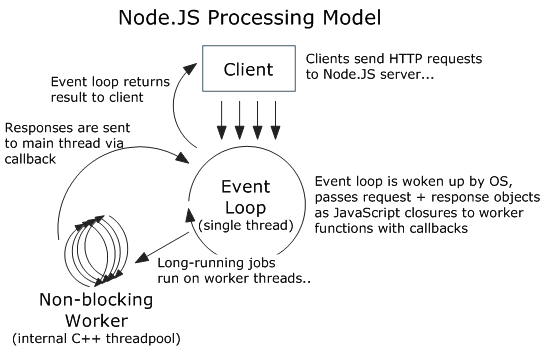
\includegraphics[scale=0.75]{nodejs-flow.png}
\end{figure}

\subsubsection{Socket.io}
\label{subsub:socketio}

Socket.io to biblioteka Node.js, która zapewnia komunikację dwukierunkową między przeglądarka użytkownika, a serwerem. Co ważne, sposób wykorzystania biblioteki zarówno po stornie serwera, jak i klienta jest taki sam. Komunikacja zapewniana jest przez wspierane sposoby opisane w podrozdziale \ref{sub:communication-methods})\footnote{http://socket.io/\#browser-support}:

\begin{enumerate}
  \item WebSocket
  \item Adobe® Flash® Socket
  \item AJAX long polling
  \item AJAX multipart streaming
  \item Forever Iframe
  \item JSONP Polling
\end{enumerate}

Przykładowy node.js kod po stronie serwera:

\lstinputlisting[language=JavaScript]{assets/src/socketio-example-server.js}

Powyższy kod uruchamia serwer nasłuchujący na porcie 8081, i przyjmuje zgłoszenia. Gdy klient się podłączy, dodawany jest callback na rzecz obiektu klienta \lstinline{socket} na wiadomość nazwaną \emph{the message from client}, który jest wykonywany, gdy wiadomość o takim identyfikatorze nadejdzie, za pomocą konstrukcji \lstinline{socket.on('the_message_from_client', function(data)}. Wysyłanie wiadomości podłączonemu klientowi odbywa się poprzez wywołanie metody emit na rzecz obiektu klienta socket \lstinline{socket.emit('the_message_from_server', function(data)} , która przyjmuje argument jako nazwę wiadomości \emph{the message from server} oraz drugi w postaci obiektu JavaScript, który zostanie zserializowany do formatu JSON i wysłany jako tekst, gdzie po stornie klienta zostanie zdeserializowany i zinterpretowany również jako obiekt JavaScript.

Przykładowy kod po stornie klienta:

\lstinputlisting[language=JavaScript]{assets/src/socketio-example-client.js}

Kod jest bliźniaczo podobny do kodu uruchamianego na serwerze. Klient ustanawia połączenie do adresu podanego jako argument funkcji \lstinline{connect}. Domyślnie używany jest protokół WebSocket ws://, można skorzystać z szyfrowanego protokołu wss://\footnote{analogiczny http:// do https://} wskazując go przed nazwę hosta. Istnieje możliwość skonfigurowania połączenia, np wskazać, czy ma zostać podjęta próba ponownego połączenia przy jego utracie.

\subsubsection{Skalowanie}
\label{subsub:scalability}

% http://book.mixu.net/node/ch13.html

\section{Sterowanie ekranem}
\label{sec:component-controll-remote-screen} % marker umożliwiający odwolanie z sekcji architektura

\subsection{Wstęp}

Klient to komputer podłączony bezpośrednio do ekranu wyświetlającego obraz. Istotnymi cechami takiego urządzenia są przede wszystkim:
\begin{itemize}
	\item niska cena
	\item wystarczająca moc obliczeniowa do uruchomienia przeglądarki, oraz prostej gry w technologi Flash, lub HTML5
	\item duża dostępność
	\item mały rozmiar
\end{itemize}

Głównym zadaniem klientów jest komunikacja serwerem poprzez sieć Ethernet w celu wyświetlania obrazu na podłączonym do klienta ekranie, oraz możliwość sterowania urządzeniami wejścia (klawiatura, myszka) poprzez udostępniony interfejs w sieci Ethernet.


\subsection{Hardware}

\subsubsection{Architektura procesora}
Jeśli chodzi o wybór architektury procesora wybór był całkiem prosty, za sprawą sporej liczby dostępnych urządzeń dostępnych w tej architekturze (32 bitowa architektura ARM\footnote{Advanced RISC Machine} jest najczęściej stosowaną architekturą w urządzeniach mobilnych\cite{acm}), jak i uzasadnioną ich popularnością. Architektura ARM cechuje cię niskim poborem energii, dużą niezawodnością w systemach wbudowanych, oraz dla praktycznie wszystkich dostępnych na rynku procesorów możliwością instalacji w pełni funkcjonalnego systemu operacyjnego.
Procesory oparte o architekturę ARM przetwarzają instrukcje z wykorzystaniem mechanizmu potokowania. Procesor może wykonywać trzy rodzaje instrukcji:
\begin{itemize}
	\item 32-bitowe ARM
	\item 64-bitowe ARM (Apple A7)
	\item 16-bitowe Thumb (oraz Thumb2)
\end{itemize}

\\
Firma ARM projektuje rdzenie procesorów i sprzedaje je producentom. Producenci z kolei tworzą urządzenia typu SoC\footnote{System on Chip} - dodawane są bloki funkcyjne, jednostki wektorowe czy procesory sygnałowe. Istnieje też spora lista firm, które projektują swoje rdzenie wykorzystujące zbiór instrukcji ARM m.in. Apple, XScale, czy Faraday.
\\
Istotną cechą, którą powinien posiadać procesor ARM jest jednostka MMU\footnote{Memory Managment Unit}. Jest to jednostka odpowiadająca za dostęp do zewnętrznej pamięci, translacje adresu wirtualnego na fizyczny, oraz kontroli uprawnień dostępu do pamięci. Wiele rdzeni ARM nie jest wyposażonych w tą jednostkę, która staje się obligatoryjna podczas gdy chcemy zainstalować system operacyjny Linux. 
\\

Po wyborze architektury procesora należy wybrać rodzinę procesora. Rodzina Cortex jest kolejną generacją procesorów po ARM7, ARM9, czy ARM11.

\begin{figure}
\begin{center}
	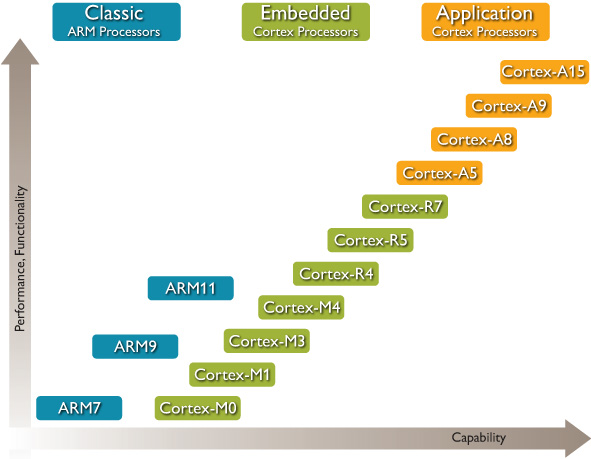
\includegraphics[scale=0.6]{ARM_Comparison}
\end{center}
\caption{Porównanie rodzin architektury ARM}
\label{fig:ARM_Comp}
\end{figure}

Zgodnie z tym co można zauważyć na rysunku~\ref{fig:ARM_Comp} architektura Cortex jest rodziną cechującą się wyższym od swoich poprzedników współczynnikiem wydajności na cykl zegara i niższym zużyciem energii.

Na rynku można wyodrębnić 3 główne chipy bazujące na architekturze ARM:
\begin{itemize}
	\item Allwinner (sunxi)
	Przykładowe produkty:
	\begin{itemize}
		\item Hackberry A10
		\item MK802
	\end{itemize}

	Chipy Allwinnera charakteryzują się stosunkowo najniższą ceną, oba przedstawione wyżej modele bazują na rdzeniu Cortex-A8 taktowane zegarem 1GHz, oraz dysponujące 1GB pamięci operacyjnej. Wyposażone są także w procesor graficzny ARM Mali 400
	
	\item Freescale i.MX6 (imx)
	Przykładowe produkty:
	\begin{itemize}
		\item MarS
		\item IMX53QSB
	\end{itemize}
	\item TI OMAP3/4
	Przykładowe produkty:
		\begin{itemize}
			\item Beaglebone Black
			\item Panda Board
		\end{itemize}
	Ta rodzina zyskała bardzo dużą popularność. Chipy OMAP3 wyposażone są w zmiennoprzecinkową jednostkę oraz zestaw instrukcji wektorowych NEON. Główną cechą tego rozwiązania jest dużo wydajność operacji przy zachowaniu prostoty ich programowania.
\end{itemize}



\subsection{System operacyjny Linux}

Nie dysponując zbyt dużą mocą obliczeniową, małą pamięcią operacyjną, oraz niewielką przestrzenią dyskową należy dobrze dobrać, oraz skonfigurować system operacyjny. Do tego celu wybrano dystrybucje linuksa - Debian. Cechuje się ona przede wszystkim wysoką stabilnością (bardzo często wybierana jako system serwerowy), oraz sporą społecznością programistów rozwijających tą dystrybucje co przekłada się na mnogość dostępnych pakietów przygotowanych specjalnie dla tej wersji systemu Linux. Wreszcie system Debian jest wysoce konfigurowalny - oparty o jądro Linux, daje użytkownikowi możliwość zbudowania systemu od podstaw.

Do zbudowania systemu Linux opartego o architekturę ARM posłużono się istniejącą instalacją Debian na komputerze osobistym. 

\subsubsection{Przygotowanie bazowej wersji systemu}

\begin{figure}
\begin{center}
    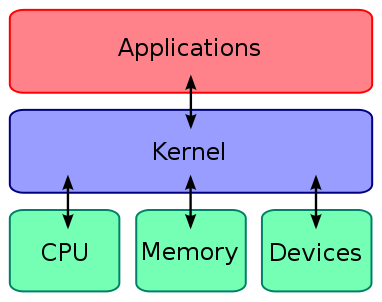
\includegraphics[scale=1]{kernel}
\end{center}
\caption{Działanie jądra systemu Linux}
\label{fig:kernel}
\end{figure}

Jądro \footnote{ang. \emph{Kernel}} systemu Linux jest centralnym miejscem systemu operacyjnego. Jak zaprezentowano na rysunku ~\ref{fig:kernel} jest ono najniżej usytuowaną warstwą systemu operacyjnego odpowiadającą za komunikację z procesorem, pamięcią, czy urządzeniami zewnętrznymi. Kernel m.in. przydziela odpowiednią ilość pamięci operacyjnej dla każdej aplikacji, obsługuje komunikaty i komunikacje między procesorową.

Pierwotnym twórcą jądra Linux jest programista pochodzenia duńskiego Linus Torvalds, natomiast obecnie jądro systemu Linux jest rozwijane przez programistów z całego świata. Jego aktualną wersje można pobrać z oficjalnego otwartego repozytorium github.

\\
\\


Instalując dystrybucję linuksa na komputerze PC zwykle nie ma większego sensu by kompilować jądro. Większość dystrybucji udostępnia gotowy obraz, który zawiera podstawowe programy i usługi niezbędne do instalacji systemu operacyjnego z środowiskiem graficznym. W przypadku systemu wbudowanego wygląda to nieco inaczej. Nie ma jednego gotowego obrazu pasującego do wszystkich jednoukładowych komputerów. Dlatego też w niniejszym rozdziale opisana zostanie instalacja systemu Linux od podstaw \footnote{ang. \emph{Linux From Scratch}}.
\\
\\

Na początku należy stworzyć sobie miejsce na dysku, w którym system będzie budowany - \lstinline|mkdir ~/ARM_DEBIAN && alias arm='cd ~/arm' && arm|.

\subsubsection{Przygotowanie karty SDHC}


System debian zostanie zainstalowany na karcie SDHC \footnote{ang. \em{Secure Digital High Capacity}}, po czym zostanie uruchomiony na urządzeniu Rickomagic MK802 II. Komputer ten opiera się o architekturę ARM Cortex-A8, bazuję na chipie firmy AllWinner sun4i.
\\
\\
	\begin{table}[t]
		\centering
		\caption{SD Card Layout}
		\label{tab:sd-layout}
	\begin{tabular}{|c|c|c|}
	\hline
	\textbf{Start} & \textbf{rozmiar} & \textbf{użycie} \\ 
	\hline
	0 & 8KB & Nieużywane, dostępne do układu partycji \\
	\hline
	8 & 24KB & SPL \footnote{ang. emph{Secondary Program Loader}} \\
	\hline
	32 & 512KB & u-boot \\
	\hline
	544 & 128KB & Środowisko \\
	\hline
	672 & 352KB & Zarezerwowana \\
	\hline
	1024 & - & Dostępne dla partycji \\
	\hline
	
	
\end{tabular}
\end{table}

\\
\\
Po włożniu karty SD do czytnika kart pamięci i podłączenia go do komputera, należy sprawdzić i upewnić się jak nazywa się podłączone urządzenie. Jest to o tyle ważne gdyż w systemach linux montowane jest w tym samym katalogu i zwykle z tym samym przedrostkiem co dysk twardy komputera. Gdyby karta pamięci zostałaby źle zidentyfikowana mogło być dojść do bezpowrotnego usunięcia danych z dysku twardego komputera. Po włożeniu karty do czytnika nazwę urządzenia w komputerze można sprawdzić za pomocą polecenia \lstinline|sudo dmesg| wyświetlając systemowy bufor komunikatów. 
\\
\\
Pierwszym krokiem w przygotowaniu systemu jest skasowanie pierwszych 2047 sektorów pamięci na karcie pamięci - zgodnie z tym co widzimy na tabeli ~\ref{tab:sd-layout} pierwszy MB pamięci (2048 sektorów * 512B) jest zarezerwowany dla danych potrzebnych do uruchomienia systemu z karty.
\\
\begin{lstlisting}[language=bash]
dd if=/dev/zero of=/dev/sdh bs=512 count=2047
\end{lstlisting}
\\
Następnie za pomocą programu do partycjonowania (np. fdisk) należy utworzyć dwie partycje - pierwszą zaczynającą się w 2048 sektorze bądź dalszym o wielkości 16MB w której będzie przechowywane jądro (uImage), plik boot.scr i script.bin, oraz drugą partycja zajmująca pozostałą część karty, która będzie przechowywała główny system plików.
\\

\begin{lstlisting}[language=bash]
mkdir mnt
sudo mkfs.vfat /dev/sdh1
sudo mount /dev/sdh1 mnt
\end{lstlisting}

W powyższym fragmencie tworzony jest katalog mnt w domowym folderze projektu, pierwsza partycja na karcie jest formatowana do systemu plików FAT, później montowana jest do katalogu mnt.


Niezbędnymi narzędziami do zainstalowania systemu są:
\begin{itemize}
	\item {\lstinline|gcc-x-arm-linux-gnueabi|}  - kompilator dla architektury ARM. Fraza eabi, znajdująca się na końcu nazwy tego pakietu to pewien standard opracowany przez firmę ARM. ABI  \footnote{ang. \emph{Application Binary Interface}} jest to zestaw reguł i ustawień kompilacji, które decydują o tym jak dany program współpracuje z innymi bibliotekami, czy aplikacjami. Programy skompilowane przy pomocy kompilatora używającego standardu EABI są przenośne pomiędzy systemami operacyjnymi (jedyną barierą są biblioteki z którymi współpracuje dany program).
	\item {\lstinline|build-essential|} - jak sama nazwa wskazuje jest to zbiór pakietów niezbędnych do budowania oprogramowania. Zależnościami tego pakietu to m.in. g++, libc, czy make.
	\item {\lstinline|git|} - system kontroli wersji
	\item {\lstinline|u-boot-tools|} - zestaw narzędzi do bootloadera, który zostanie opisany w dalszej części pracy.
\end{itemize}


\subsubsection{Bootloader}

W komputerach o architekturze ARM proces uruchamiania systemu operacyjnego oparty jest o program uruchomieniowy Bootstrap. Na samym początku szuka on programu uruchomieniowego w pierwszym sektorze pamięci NAND, następnie przeszukiwana jest karta SD/MMC (szukając pliku boot.bin na pierwszej partycji karty), pamięć Dataflash, i jako ostatnia pamięć EEPROM podłączona do magistrali I2C. Jeżeli w którejś z tych lokacji bootstrap znajdzie prawidłowy kod, to jest on kopiowany do wewnętrznej pamięci operacyjnej procesora (SRAM) i tam uruchamiany. W następnej kolejności uruchamiany jest bootloader pierwszego poziomu, jest to zwykle mały program, którego zadaniem jest inicjalizacja pamięci RAM, oraz jednej z pamięci nieulotnych, a następnie uruchomienie bootloadera drugiego poziomu.
Najpopularniejszym bootloaderem w systemach opartych o architekturę ARM jest u-boot. Głównym zadaniem bootloadera drugiego poziomu jest wczytanie pliku jądra systemu. Za pomocą u-boota można go wczytać z karty SD, czy nawet poprzez serwer ftp.
\\
\\
Aktualną wersję u-boota można pobrać i skompilować za pomocą poleceń:

\begin{lstlisting}[language=bash]
git clone https://github.com/linux-sunxi/u-boot-sunxi.git
cd uboot-allwinner
git checkout sun4i
make sun4i CROSS_COMPILE=arm-linux-gnueabi-
\end{lstlisting}

\\
\\
W pierwszej lini pobierane jest repozytorium, w linii 3 z kolei przełączamy pobrane repozytorium na odpowiednią gałąź, wreszcie w linii 4 kompilujemy bootloader na architekturę \lstinline|sun4i| używając do tego celu kompilatora \lstinline|arm-linux-gnueabi-gcc|.

Po skompilowaniu można wgrać niezbędny pliki na kartę SD:

\begin{lstlisting}[language=bash]
dd if=spl/sun4i-spl.bin of=/dev/sdh bs=1024 seek=8  (if sun4i-spl.bin not found, try sunxi-spl.bin)
dd if=u-boot.bin of=/dev/sdh bs=1024 seek=32
\end{lstlisting}
\\

Plik boot.cmd jest plikiem konfiguracyjnym, używanym przez program bootstrap:

\begin{lstlisting}[language=bash]
setenv console 'ttyS0,115200'
setenv root '/dev/mmcblk0p2'
setenv panicarg 'panic=10'
setenv extra 'rootfstype=ext4 rootwait'
setenv loglevel '8'
setenv setargs 'setenv bootargs console=${console} root=${root} loglevel=${loglevel} ${panicarg} ${extra}'
setenv kernel 'uImage'
setenv boot_mmc 'fatload mmc 0 0x43000000 script.bin; fatload mmc 0 0x48000000 ${kernel}; bootm 0x48000000'
setenv bootcmd 'run setargs boot_mmc'
\end{lstlisting}

Stworzony plik boot.cmd należy skompilować do formatu boot.scr i skopiować na kartę SD:

\begin{lstlisting}[language=bash]
mkimage -A arm -O u-boot -T script -C none -n "boot" -d boot.cmd boot.scr
sudo cp boot.scr mnt/
\end{lstlisting}


\subsubsection{Kompilacja jądra i przygotowanie plików konfiguracyjnych}

Jądro systemu wykrywa i inicjuje sprzęt, oraz uruchamia proces init, który może być procesem dowolnego programu, natomiast aby uzyskać funkcjonalny system proces ten powinien zająć się uruchamianiem m.in. skryptów startowych, czy odbieraniem kodów wyjścia z zakończonych procesów.

Pierwszym krokiem jest ściągnięcie kodu źródłowego jądra, z racji tego, że architektura ARM Allwinner sun4i nie jest oficjalnie wspierana przez repozytorium w którym znajduję się jądro linuksa posłużono się repozytorium wywodzącym się z niego przystosowanym do potrzeb tej architektury.

Aktualną wersję jądra można pobrać za pomocą polecenia: \lstinline|git clone https://github.com/linux-sunxi/linux-sunxi|, a następnie przełączyć się na odpowiednią gałąź kodu: \lstinline|git checkout sunxi-3.4|. By skompilować jądro należy wykonać polecenia:

\begin{lstlisting}[language=bash]
make ARCH=arm CROSS_COMPILE=arm-linux-gnueabi- sun4i_defconfig
make ARCH=arm CROSS_COMPILE=arm-linux-gnueabi- -j16 uImage modules
make ARCH=arm CROSS_COMPILE=arm-linux-gnueabi- INSTALL_MOD_PATH=output modules_install

arm
sudo cp linux-allwinner/arch/arm/boot/uImage mnt/
\end{lstlisting}

W pierwszej linii generowana jest standardowa konfiguracja jądra dla danej platformy. Parametr \lstinline|ARCH=arm| określa architekturę jądra. Parametr \lstinline|CROSS_COMPILE=arm-linux-gnueabi-| określa przedrostek cross kompilatora, używany przy budowaniu i przy instalacji (czyli cross kompilator dla poleceń w liniach 1-3 to arm-linux-gnueabi-gcc).
\\
\\
W linii drugiej budowane są moduły jądra, oraz plik z jądrem, następnie dodawana do niego jest suma kontrolna, oraz informacje wymagane przez bootloader. Parametr j16 jest parametrem programu \lstinline|make| określającym ile jednocześnie zadań może być uruchamianych, przez zadanie w przypadku programu \lstinline|make| rozumiane jest rozwiązanie jednej zależności. Program make za pomocą grafu zależności określa kolejność wykonywanych zadań.
\\
\\
Komenda z linii trzeciej instaluje moduły w zadanej lokacji.
\\
Plik script.bin jest plikiem konfiguracyjnym dla danej platformy. Można go wygenerować samemu, dokumentacja znajduję się na oficjalnej stronie architektury sunxi - http://linux-sunxi.org/Fex_Guide. a następnie skompilować plik konfiguracyjny do formatu bin za pomocą narzędzia \lstinline|fex2bin|. W pliku tym konfigurowane są wartości typowe dla urządzenia tj. adres MAC komputera, czy maksymalna rozdzielczość.  W internecie istnieje wiele gotowych plików konfiguracyjnych dla komputera MK 802 II, na potrzeby niniejszej pracy konfiguracja została pobrana ze strony - http://dl.miniand.com/gamboita/script-mk802ii-1080p60.7z. 

Po wygenerowaniu pliku należy go skopiować na kartę pamięci do pierwszej partycji \lstinline|sudo cp script.bin mnt/script.bin|. 

Tym sposobem zakończono modyfikacje na partycji pierwszej - przygotowano i skopiowano plik jądra, plik konfiguracyjny urządzenia, oraz plik konfiguracyjny bootloadera. 

By odmontować partycje należy wpisać \lstinline|sudo umount mnt|

\subsubsection{Przygotowanie głównego systemu plików}

Pakiet debootstrap jest to narzędzie, który pozwala zainstalować bazowy system debiana w podkatalogu na obecnie zainstalowanym systemie. Jest on dostępny w oficjalnych repozytoriach debiana.

\begin{lstlisting}[language=bash]
sudo apt-get install debootstrap
mkdir debian-rootfs
cd debian-rootfs
dd if=/dev/zero of=debian_rootfs.img bs=1M count=1024
sudo mkfs.ext3 -F debian_rootfs.img
mkdir mnt
sudo mount -o loop debian_rootfs.img mnt
sudo debootstrap --verbose --arch armel --variant=minbase --foreign squeeze mnt http://ftp.debian.org/debian
\end{lstlisting}

W liniach 4-8 powyższego listingu tworzony jest pusty obraz systemu sformatowany do formatu ext3, oraz zamontowany do katalogu mnt. Za pomocą wspomnianego wcześniej narzędzia debootstrap ściągnięto z oficjalnej strony dystrybucji bazowy system operacyjny, oraz zainstalowano go.


\begin{lstlisting}[language=bash]
sudo apt-get install -t testing qemu-user-static
sudo apt-get install binfmt-support
sudo modprobe binfmt_misc
sudo cp /usr/bin/qemu-arm-static mnt/usr/bin
sudo mkdir mnt/dev/pts
sudo mount -t devpts devpts mnt/dev/pts
sudo mount -t proc proc mnt/proc
sudo chroot mnt/
/debootstrap/debootstrap --second-stage
\end{lstlisting}

Pakiet \lstinline|quemu-user-static| pozwala na emulowanie binarek zbudowanych statycznie. Ogólnie rzecz biorąc pozwala na uruchamianie procesów linuksowych na procesorze pod który nie zostały one skompilowane. Pakiet binfmt-support pozwala na obsługe dodatkowych formatów binarnych. Za pomocą polecenia \lstinline|modprobe| moduł obsługi dodatkowych formatów binarnych zostaje włączony jako moduł do jądra. Polecenie z linii 4 kopiuje aplikacje do nowo stworzonego systemu. Linie 5-6 to przygotowaniu interfejsu tzw. pseudoterminala. Poprzez zamontowanie systemu plików \lstinline|/proc| do nowo powstającego systemu, po wykonaniu chroota będzie możliwość korzystania z informacji dostarczonych przez jądro systemu. Wreszcie wykonujemy polecenie \lstinline|chroot| \footnote{ang. \emph{change root}}, które jak sama nazwa wskazuje zmienia główny system plików. Po wykonaniu przed ostatniego polecenia linia poleceń powinna wyświetlić komunikat \lstinline|I have no name!@hostname:/#|, ostatnie polecenie uruchamia wszystkie skrypty konfiguracyjne, które muszą zostać wykonane na architekturze docelowej (dlatego właśnie skopiowany został do /usr/bin program qemu-user-static). Mając uruchomiony system na komputerze wykonano podstawową konfiguracje dla systemu debian.
\\
Edycja repozytoriów menadżera pakietów:
\begin{lstlisting}[language=bash]
cd /root
cat <<koniec > /etc/apt/sources.list
deb http://security.debian.org/ squeeze/updates main contrib non-free
deb-src http://security.debian.org/ squeeze/updates main contrib non-free
deb http://ftp.debian.org/debian/  squeeze main contrib non-free
deb-src http://ftp.debian.org/debian/  squeeze main contrib non-free
koniec
apt-get update
\end{lstlisting}

Konfiguracja języka i podstawowych narzędzi:
\begin{lstlisting}[language=bash]
export LANG=C
apt-get install apt-utils
apt-get install dialog
apt-get install locales
cat <<END > /etc/apt/apt.conf.d/71mele
APT::Install-Recommends "0";
APT::Install-Suggests "0";
END
dpkg-reconfigure locales
export LANG=pl_PL.UTF-8
apt-get install dhcp3-client udev netbase ifupdown iproute openssh-server \
    iputils-ping wget net-tools ntpdate uboot-mkimage uboot-envtools vim nano less X
\end{lstlisting}

Po skonfigurowaniu usług internetowych, i konta roota, należy wyjść z trybu \lstinline|chroot|, oraz odmontować partycję:

\begin{lstlisting}[language=bash]
exit
sudo umount mnt/proc
sudo umount mnt/dev/pts
\end{lstlisting}

Ostatnim elementem w przygotowywaniu drugiej partycji jest zainstalowaniu modułów jądra na głównym systemie plików, poleceniem: \lstinline|sudo make ARCH=arm CROSS_COMPILE=arm-linux-gnueabi- INSTALL_MOD_PATH=../debian-rootfs/mnt modules_install|.

Po zainstalowaniu modułów pozostaje tylko przygotować drugą partycje na karcie SD i zainstalować przygotowany system plików:
\begin{lstlisting}[language=bash]
cd /home/share/mele-hacking
mkdir mnt2
sudo mkfs.ext4 /dev/sdh2 
sudo mount /dev/sdh2 mnt2
sudo cp -a debian-rootfs/mnt/* mnt2/
sudo umount mnt2
sudo umount debian-rootfs/mnt
\end{lstlisting}

\subsubsection{Oprogramowanie klienckie dla systemu Linux}

Oprogramowanie klienckie składa się z następujących komponentów:
\begin{description}
	\item[serwer] \hfill \\
Kod źródłowy serwera znajduję się w załączniku ~\ref{app:server_c}, jest on wspólny dla wszystkich platform unixowych.		
	\item[generator zdarzeń wejścia] \hfill \\ 
		Program generujący zdarzenia urządzeń wejścia na podstawie danych otrzymanych z serwera. W platformie Linux wykorzystano moduł jądra \lstinline|uinput|. Uinput to moduł pozwalający na generowanie zdarzeń symulujących urządzenia wyjścia. Moduł ten tworzy specjalny plik urządzenia w katalogu \lstinline|/dev|. Plik ten jest wirtualnym interfejsem co znaczy, że nie jest połączony z żadnym fizycznym urządzeniem.

		Jednym z zadań generatora jest ustalenie rozdzielczości ekranu na którym wyświetlany jest obraz. Informacja ta jest niezbędna gdyż koordynaty wysyłane przez serwer są podawane absolutnie, oraz z przedziału od 0 do 1 (ze względu na to, że informacja ta nie może być uzależniona od rozdzielczości monitora). Na platformie Linux rozdzielczość uzyskiwana jest za pomocą następującego polecenia:
		\begin{lstlisting}[language=bash]
		"xdpyinfo -display :0 | sed 's/^ *dimensions: *\\([0-9x]*\\).*/\\1/;t;d'";
		\end{lstlisting}
		Program xdpyinfo jest to aplikacja służąca do wyświetlania informacji o serwerze X, z kolei za pomocą wyrażenia regularnego i programu sed wyłuskano tylko niezbędne informacje dotyczące rozdzielczości ekranu.

		Istotnym elementem w pisaniu programu generującego zdarzenia urządzeń wejścia jest odbiór danych z serwera, opisanego w załączniku ~\ref{app:server_c}. Program ten wysyła dane do deskryptora pliku o nazwie \lstinline|STDIN_FILENO|. Nie jest to bynajmniej to samo co wskaźnik do pliku o nazwie \lstinline|stdin| przez co nie jest możliwe użycie funkcji wysokiego poziomu jak lstinline|scanf| do wczytania danych. Niezbędne jest użycie funkcji \lstinline|read|, a następnie użycie funkcji \lstinline|sscanf| w celu sformatowaniu danych co pokazuje poniższy fragment kodu:

		\begin{lstlisting}[language=c]
			read(STDIN_FILENO, buffer, sizeof(buffer));
			int result = sscanf(buffer, "x:%lf:y:%lf;", &xTmp, &yTmp);
			int x = xTmp * dim[0];
			int y = yTmp * dim[1];
		\end{lstlisting}

		Wczytane koordynaty należy wysłać jako zdarzenia do modułu \lstinline|uinput|. 
		
		\begin{lstlisting}[language=c]
		#include <linux/input.h>
		#include <linux/uinput.h>
		int fd = open("/dev/input/uinput", O_WRONLY | O_NONBLOCK);
		ret = ioctl(fd, UI_SET_EVBIT, EV_ABS);
		
		...

		struct input_event ev, synEv;
	

		...
		memset(&ev, 0, sizeof(ev));
		ev.type = EV_ABS;
		ev.code = ABS_X;
		ev.value = x;
		if(write(fd, &ev, sizeof(struct input_event)) < 0)
            die("error: write");  

		memset(&synEv, 0, sizeof(struct input_event));
        synEv.type = EV_SYN;
        synEv.code = 0;
        synEv.value = 0;
        if(write(fd, &synEv, sizeof(struct input_event)) < 0)
            die("error: write");

		...
		//sending y coordinate


		\end{lstlisting}
		Na początku należy włączyć niezbędne nagłówki (linie 1-2), następnie otworzyć plik urządzenia \lstinline|uinput|, do którego będą wysyłane zdarzenia urządzeń wejścia. W linii 4 powyższego listingu, włączono możliwość wysyłania zdarzeń ruchów myszką podając koordynaty absolutne. Struktury zadeklarowane w linii 8 zawierają 3 pola 
		\begin{itemize}
			\item \lstinline|type| - typ zdarzenia (\lstinline|EV_KEY|, \lstinline|EV_ABS|, \lstinline|EV_REL|)		
			\item \lstinline|code| - dla zdarzeń klawiatury jest to kod klawisza, natomiast dla zdarzeń myszy jest to oś.
			\item \lstinline|value| - dla zdarzeń klawiatury 1 oznacza przyciśnięcie klawisza, a 0 puszczenie, dla zdarzeń myszy jest to z kolei wartość reprezentująca koordynatę.
		\end{itemize}
		Po wypełnieniu struktury odpowiednimi wartościami należy wysłać je do wcześniej otwartego deskryptora pliku (\lstinline|fd|), a następnie wypełnić i wysłać strukturę synchronizującą (\lstinline|evSyn|), której zadaniem jest zatwierdzenie, oraz realizacja wszystkich dotychczasowo wysłanych zdarzeń. 
	\item[serwer X] \hfill \\
		Moduł ten opisany jest bardziej szczegółowo w załączniku ~\ref{app:X Window System}.


\end{itemize}


\subsection{System operacyjny Mac OS X}
W niniejszym podrozdziale niezostanie omówiony proces instalacji systemu Mac OS X na żadnym z jednoukładowych komputerów gdyż jest to niemożliwe ze względu na to, że system Mac OS X jest dedykowanym oprogramowaniem dla komputerów firmy Apple. 
\subsubsection{Oprogramowanie klienckie dla systemu Linux}

Serwer odbierający zdarzenia jest wspólny dla wszystkich systemów unixowych i został opisany w załączniku ~\ref{app:server_c}.
\\
Kod generator zdarzeń dla systemu Mac OS X jest nieco prostszy aniżeli dla systemu Linux. Bazuje on na zdarzeniach z biblioteki CoreGraphics. Tak jak i dla systemu Linux istotnym elementem jest odczytanie rozdzielczości ekranu. Jest to wykonane za pomocą polecenia:
\begin{lstlisting}
system_profiler SPDisplaysDataType | grep Resolution | sed 's/[^0-9 ]*//g' | sed -e 's/^[ \t]*//' | sed 's/  */x/g'
\end{lstlisting}
Format wyniku powyższego polecenia jest dokładnie taki sam jak dla instrukcji analogicznej w systemie Linux.
\\
Kod programu odpowiadający za wygenerowanie zdarzenia na podstawie koordynatów znajduję się na poniższym listingu:
\begin{lstlisting}
		CGEventRef move1 = CGEventCreateMouseEvent(
		    NULL, kCGEventMouseMoved,
			CGPointMake(x, y),
			kCGMouseButtonLeft
		);

		CGEventPost(kCGHIDEventTap, move1);

		CFRelease(move1);
\end{lstlisting}

\\
Funkcja \lstinline|CGEventCreateMouseEvent| tworzy nowe zdarzenie, polegające na przesunięciu kursora myszy do zadanej lokacji.



\subsection{Serwer zarządzania infrastrukturą}

\subsubsection{Zdalne sterowanie programami}

Zgodnie z diagramem znajdującym się w załączniku ~\ref{app:network_diagram_app}, serwer www zarządzający infrastrukturą niekoniecznie musi być umieszczony na tym samym urządzeniu co serwer wyświetlania, z racji tego serwer www musi sterować tym serwerem przez protokół ssh\footnote{ang. \emph{Secure Shell} - to standard protokołów komunikacyjnych używanych w sieciach komputerowych TCP/IP, w architekturze klient-serwer.\cite{ssh-wiki}}.
Do logowania do zdalnej stacji roboczej na serwerze www użyto biblioteki \lstinline{scala-ssh}. Poniższy fragment kodu źródłowego przedstawia metode obsługującą logowanie do aplikacji webowej.

\begin{lstlisting}
def signin() = Action.async(parse.json) {
    implicit request =>
    {
      var login : String = ""
      var f = Future[Boolean] {
        var sshIPAddress = (request.body \ "ip_address").asOpt[String]
        var someLogin = (request.body \ "login").asOpt[String]
        var password = (request.body \ "password").asOpt[String]
        if (sshIPAddress.isEmpty || someLogin.isEmpty || password.isEmpty) {
          false
        }
        else {
          login = someLogin.get
          SSHUser.connect(sshIPAddress.get, someLogin.get, password.get)
        }
      }
      f.map(fut => {
        var res = Ok(toJson(Map("success" -> fut)))
        if (fut) {
          res.withSession(Security.username -> login)
        }
        else
          res
      })
    }
  }
\end{lstlisting}

Metoda odpowiada w formacie JSON\footnote{ang. \emph{JavaScxript Object Notation} - lekki format wymiany danych.}, gdyż żądanie, które wysyła przeglądarka internetowa, jest wysłane w technice AJAX \footnote{ang. \emph{Asynchronous JavaScript and XML.}}. Dane, które zostają wysłane do serwera, również są w formacie JSON, po wyłuskaniu danych do odpowiednich zmiennych w linii 14 wykonywana jest próba logowania do zdalnej stacji roboczej. Cała metoda \lstinline{signin} jest asynchroniczna, przez co wykonanie metody \lstinline{connect} nie blokuje wątku. Dzięki takiemu podejściu wątek, który obecnie czeka na odpowiedź z serwera, może obsłużyć kolejne żądanie.

\par

Po pomyślnym zalogowaniu użytkownik może dodać nowych klientów oraz uruchomić na nich aplikacje wybierając je z listy.

\begin{lstlisting}
  def runXApp(app: PNPProcessApp) {
    currentProcesses.foreach(p => p.kill)
    if (app.name != PNPProcessApp.none.name) {
      SSHUser.sshClient.exec(app.toString + " -display " + ip_screen_address)
    }
  }
\end{lstlisting}

Powyższa metoda jest wywołana za każdym razem gdy użytkownik przełączy aplikację. W linii drugiej 'zabijana' jest dotychczasowo uruchomiona aplikacja, a następnie przy pomocy biblioteki \lstinline{scala-ssh} wywoływana jest aplikacja wybrana z listy, z parametrem display określającym miejsce wyświetlenie aplikacji.






\newpage
\section{Testowanie i uruchamianie}

Testowanie i uruchamianie to konieczna część przebiegu prac. Z racji tego, że stworzony projekt nie ma specyfiki monolitycznego programu, a wręcz rozproszenie kodu pomiędzy systemami jest znaczne, w głównej mierze dział skoncentrowany jest zstępującym testom integracyjnym w punktach zestyku komponentów.

Wykonane testy zakładały zarówno poprawną, jak i niepoprawną konfigurację systemu.

Istotnym dla pilotów sterujących były testy funkcjonalne na urządzeniach mobilnych o ekranach różnej rozdzielczości oraz różnych systemach operacyjnych w starszych i nowszych wersjach. Urządzenia mobilne, na których zostały przeprowadzone testy:
\begin{itemize}
	\item iPhone 5, system operacyjny: iOS 7.0
	\item iPhone 4, system operacyjny: iOS 4.1 (brak obsługi Web Sockets)
	\item iPad, system operacyjny: iOS 3.1.2 (brak obsługi Web Sockets)
	\item Samsung Galaxy S III, system operacyjny: Android 4.1
	\item HTC Wildfire S, system operacyjny: Android 2.3.5 (brak obsługi Web Sockets)
\end{itemize}

\subsection{Pilot do sterowania zdalnym monitorem}

Przetestowana została:

\begin{itemize}
	\item poprawność wyświetlania się elementów strony internetowej pilota na urządzeniach mobilnych o różnych rozdzielczościach ekranu,
	\item poprawność przechwytywania i interpretacji punktów styku użytkownika z ekranem urządzenia mobilnego,
	\item poprawność działania komunikacji klienta pilota z serwerem i vice versa, sposób reagowania na otrzymywane komunikaty wg specyfikacji interfejsów,
	\item poprawność łączenia się serwera do programu generującego zdarzenia urządzeń wejścia oraz poprawność przesyłanych danych.
\end{itemize}

Wszystkie testy zostały pomyślnie zakończone.

\subsection{Gra PONG}

Przetestowana została:

\begin{itemize}
	\item poprawność wyświetlania się elementów strony internetowej pilota na urządzeniach mobilnych o różnych rozdzielczościach ekranu,
	\item poprawność przechwytywania i interpretacji punktów styku użytkownika z ekranem urządzenia mobilnego,
	\item poprawność działania komunikacji klienta z serwerem i vice versa, sposób reagowania na otrzymywane komunikaty wg specyfikacji interfejsów,
	\item poprawność łączenia się serwera do klienta wyświetlającego grę,
	\item poprawność działania klienta wyświetlającego grę, jego wyświetlania i logiki.
\end{itemize}

Wszystkie testy zostały pomyślnie zakończone, aczkolwiek sporo czasu zajęło dostosowanie wyglądu pilota pod wszystkie urządzenia mobilne. Urządzenia mobilne bez wsparcia protokołu Web Sockets generowały opóźnienia w komunikacji stosując alternatywne metody komunikacji HTTP Comet.

\subsection{Program generujący zdarzenia urządzeń wejścia}

\subsection{Serwer zarządzania infrastrukturą}

\newpage
\section{Instalacja i uruchamianie systemu}

\subsection{Uruchomienie serwera node.js}
\label{subsub:setup-server-nodejs}

Do uruchomienia serwera niezbędna jest instalacja platformy node.js w odpowiedniej wersji. W tym celu należy ściągnąć kod źródłowy z oficjalnego repozytorium (\url{https://github.com/joyent/node} oznaczony tagiem 0.10.12. Po ściągnięciu i rozpakowaniu paczki należy skompilować i zainstalować platformę poleceniami:

\begin{lstlisting}
./configure
make
make install
\end{lstlisting}

Po pomyślnej instalacji należy ściągnąć repozytorium projektu dostępne po adresem - \url{https://github.com/athlan/remotely}. By rozwiązać wszystkie zależności projektu należy w katalogu z projektem wykonać polecenie \lstinline{npm install}.
\par
Do uruchomienia aplikacji pozostaje jeszcze uruchomić serwer sieciowy. W załączniku ~\ref{app:apache} omówiona została instalacja, oraz konfiguracja serwera Apache.
\par
Przed ostatnim krokiem w konfiguracji serwera jest wyedytowanie pliku index.html w głównym katalogu projektu remotely. Atrybuty przy znaczniku body to:
\begin{description}
	\item[data-server] \hfill \\
		adres komputera wraz z numerem portu, na którym jest uruchomiony serwer sieciowy
	\item[data-server-remote-host] \hfill \\
		adres klienta na który wysyłane będą zdarzenia urządzeń wejścia.
	\item[data-server-remote-port] \hfill \\
		numer portu klienta
\end{description}
\par
Po skonfigurowaniu serwera pozostaje go tylko uruchomić poleceniem \lstinline{node server.js}.


\subsection{Przygotowanie bazowej wersji systemu Linux wyświetlającego obraz na ekranie}


Instalując dystrybucję linuksa na komputerze PC zwykle nie ma większego sensu by kompilować jądro. Większość dystrybucji udostępnia gotowy obraz, który zawiera podstawowe programy i usługi niezbędne do instalacji systemu operacyjnego z środowiskiem graficznym. W przypadku systemu wbudowanego wygląda to nieco inaczej. Nie ma jednego gotowego obrazu pasującego do wszystkich jednoukładowych komputerów. Dlatego też w niniejszym rozdziale opisana zostanie instalacja systemu Linux od podstaw \footnote{ang. \emph{Linux From Scratch}}.

\par


Na początku należy stworzyć sobie miejsce na dysku, w którym system będzie budowany - \lstinline{mkdir ~/ARM_DEBIAN && alias arm='cd ~/arm' && arm}.

\subsubsection{Przygotowanie karty SDHC}


System debian zostanie zainstalowany na karcie SDHC \footnote{ang. \em{Secure Digital High Capacity}}, po czym zostanie uruchomiony na urządzeniu Rickomagic MK802 II. Komputer ten opiera się o architekturę ARM Cortex-A8, bazuję na chipie firmy AllWinner sun4i.
\par
	\begin{table}[t]
		\centering
		\caption{SD Card Layout}
		\label{tab:sd-layout}
	\begin{tabular}{|c|c|c|}
	\hline
	\textbf{Start} & \textbf{rozmiar} & \textbf{użycie} \\ 
	\hline
	0 & 8KB & Nieużywane, dostępne do układu partycji \\
	\hline
	8 & 24KB & SPL \footnote{ang. emph{Secondary Program Loader}} \\
	\hline
	32 & 512KB & u-boot \\
	\hline
	544 & 128KB & Środowisko \\
	\hline
	672 & 352KB & Zarezerwowana \\
	\hline
	1024 & - & Dostępne dla partycji \\
	\hline
	
	
\end{tabular}
\end{table}

\par
Po włożniu karty SD do czytnika kart pamięci i podłączenia go do komputera, należy sprawdzić i upewnić się jak nazywa się podłączone urządzenie. Jest to o tyle ważne gdyż w systemach linux montowane jest w tym samym katalogu i zwykle z tym samym przedrostkiem co dysk twardy komputera. Gdyby karta pamięci zostałaby źle zidentyfikowana mogło być dojść do bezpowrotnego usunięcia danych z dysku twardego komputera. Po włożeniu karty do czytnika nazwę urządzenia w komputerze można sprawdzić za pomocą polecenia \lstinline{sudo dmesg} wyświetlając systemowy bufor komunikatów. 
\par
Pierwszym krokiem w przygotowaniu systemu jest skasowanie pierwszych 2047 sektorów pamięci na karcie pamięci - zgodnie z tym co widzimy na tabeli ~\ref{tab:sd-layout} pierwszy MB pamięci (2048 sektorów * 512B) jest zarezerwowany dla danych potrzebnych do uruchomienia systemu z karty.
\par
\begin{lstlisting}[language=bash]
dd if=/dev/zero of=/dev/sdh bs=512 count=2047
\end{lstlisting}
\par
Następnie za pomocą programu do partycjonowania (np. fdisk) należy utworzyć dwie partycje - pierwszą zaczynającą się w 2048 sektorze bądź dalszym o wielkości 16MB w której będzie przechowywane jądro (uImage), plik boot.scr i script.bin, oraz drugą partycja zajmująca pozostałą część karty, która będzie przechowywała główny system plików.
\par

\begin{lstlisting}[language=bash]
mkdir mnt
sudo mkfs.vfat /dev/sdh1
sudo mount /dev/sdh1 mnt
\end{lstlisting}

W powyższym fragmencie tworzony jest katalog mnt w domowym folderze projektu, pierwsza partycja na karcie jest formatowana do systemu plików FAT, później montowana jest do katalogu mnt.


Niezbędnymi narzędziami do zainstalowania systemu są:
\begin{itemize}
	\item {\lstinline{gcc-x-arm-linux-gnueabi}}  - kompilator dla architektury ARM. Fraza eabi, znajdująca się na końcu nazwy tego pakietu to pewien standard opracowany przez firmę ARM. ABI  \footnote{ang. \emph{Application Binary Interface}} jest to zestaw reguł i ustawień kompilacji, które decydują o tym jak dany program współpracuje z innymi bibliotekami, czy aplikacjami. Programy skompilowane przy pomocy kompilatora używającego standardu EABI są przenośne pomiędzy systemami operacyjnymi (jedyną barierą są biblioteki z którymi współpracuje dany program).
	\item {\lstinline{build-essential}} - jak sama nazwa wskazuje jest to zbiór pakietów niezbędnych do budowania oprogramowania. Zależnościami tego pakietu to m.in. g++, libc, czy make.
	\item {\lstinline{git}} - system kontroli wersji
	\item {\lstinline{u-boot-tools}} - zestaw narzędzi do bootloadera, który zostanie opisany w dalszej części pracy.
\end{itemize}


\subsubsection{Bootloader}

W komputerach o architekturze ARM proces uruchamiania systemu operacyjnego oparty jest o program uruchomieniowy Bootstrap. Na samym początku szuka on programu uruchomieniowego w pierwszym sektorze pamięci NAND, następnie przeszukiwana jest karta SD/MMC (szukając pliku boot.bin na pierwszej partycji karty), pamięć Dataflash, i jako ostatnia pamięć EEPROM podłączona do magistrali I2C. Jeżeli w którejś z tych lokacji bootstrap znajdzie prawidłowy kod, to jest on kopiowany do wewnętrznej pamięci operacyjnej procesora (SRAM) i tam uruchamiany. W następnej kolejności uruchamiany jest bootloader pierwszego poziomu, jest to zwykle mały program, którego zadaniem jest inicjalizacja pamięci RAM, oraz jednej z pamięci nieulotnych, a następnie uruchomienie bootloadera drugiego poziomu.
Najpopularniejszym bootloaderem w systemach opartych o architekturę ARM jest u-boot. Głównym zadaniem bootloadera drugiego poziomu jest wczytanie pliku jądra systemu. Za pomocą u-boota można go wczytać z karty SD, czy nawet poprzez serwer ftp.

\par

Aktualną wersję u-boota można pobrać i skompilować za pomocą poleceń:

\begin{lstlisting}[language=bash]
git clone https://github.com/linux-sunxi/u-boot-sunxi.git
cd uboot-allwinner
git checkout sun4i
make sun4i CROSS_COMPILE=arm-linux-gnueabi-
\end{lstlisting}

\par

W pierwszej lini pobierane jest repozytorium, w linii 3 z kolei przełączamy pobrane repozytorium na odpowiednią gałąź, wreszcie w linii 4 kompilujemy bootloader na architekturę \lstinline{sun4i} używając do tego celu kompilatora \lstinline{arm-linux-gnueabi-gcc}.

Po skompilowaniu można wgrać niezbędny pliki na kartę SD:

\begin{lstlisting}[language=bash]
dd if=spl/sun4i-spl.bin of=/dev/sdh bs=1024 seek=8  (if sun4i-spl.bin not found, try sunxi-spl.bin)
dd if=u-boot.bin of=/dev/sdh bs=1024 seek=32
\end{lstlisting}

\par

Plik boot.cmd jest plikiem konfiguracyjnym, używanym przez program bootstrap:

\begin{lstlisting}[language=bash]
setenv console 'ttyS0,115200'
setenv root '/dev/mmcblk0p2'
setenv panicarg 'panic=10'
setenv extra 'rootfstype=ext4 rootwait'
setenv loglevel '8'
setenv setargs 'setenv bootargs console=${console} root=${root} loglevel=${loglevel} ${panicarg} ${extra}'
setenv kernel 'uImage'
setenv boot_mmc 'fatload mmc 0 0x43000000 script.bin; fatload mmc 0 0x48000000 ${kernel}; bootm 0x48000000'
setenv bootcmd 'run setargs boot_mmc'
\end{lstlisting}

Stworzony plik boot.cmd należy skompilować do formatu boot.scr i skopiować na kartę SD:

\begin{lstlisting}[language=bash]
mkimage -A arm -O u-boot -T script -C none -n "boot" -d boot.cmd boot.scr
sudo cp boot.scr mnt/
\end{lstlisting}


\subsubsection{Kompilacja jądra i przygotowanie plików konfiguracyjnych}

Jądro systemu wykrywa i inicjuje sprzęt, oraz uruchamia proces init, który może być procesem dowolnego programu, natomiast aby uzyskać funkcjonalny system proces ten powinien zająć się uruchamianiem m.in. skryptów startowych, czy odbieraniem kodów wyjścia z zakończonych procesów.

Pierwszym krokiem jest ściągnięcie kodu źródłowego jądra, z racji tego, że architektura ARM Allwinner sun4i nie jest oficjalnie wspierana przez repozytorium w którym znajduję się jądro linuksa posłużono się repozytorium wywodzącym się z niego przystosowanym do potrzeb tej architektury.

Aktualną wersję jądra można pobrać za pomocą polecenia: \lstinline{git clone https://github.com/linux-sunxi/linux-sunxi}, a następnie przełączyć się na odpowiednią gałąź kodu: \lstinline{git checkout sunxi-3.4}. By skompilować jądro należy wykonać polecenia:

\begin{lstlisting}[language=bash]
make ARCH=arm CROSS_COMPILE=arm-linux-gnueabi- sun4i_defconfig
make ARCH=arm CROSS_COMPILE=arm-linux-gnueabi- -j16 uImage modules
make ARCH=arm CROSS_COMPILE=arm-linux-gnueabi- INSTALL_MOD_PATH=output modules_install

arm
sudo cp linux-allwinner/arch/arm/boot/uImage mnt/
\end{lstlisting}

W pierwszej linii generowana jest standardowa konfiguracja jądra dla danej platformy. Parametr \lstinline{ARCH=arm} określa architekturę jądra. Parametr \lstinline{CROSS_COMPILE=arm-linux-gnueabi-} określa przedrostek cross kompilatora, używany przy budowaniu i przy instalacji (czyli cross kompilator dla poleceń w liniach 1-3 to arm-linux-gnueabi-gcc).

\par

W linii drugiej budowane są moduły jądra, oraz plik z jądrem, następnie dodawana do niego jest suma kontrolna, oraz informacje wymagane przez bootloader. Parametr j16 jest parametrem programu \lstinline{make} określającym ile jednocześnie zadań może być uruchamianych, przez zadanie w przypadku programu \lstinline{make} rozumiane jest rozwiązanie jednej zależności. Program make za pomocą grafu zależności określa kolejność wykonywanych zadań.

\par
Komenda z linii trzeciej instaluje moduły w zadanej lokacji.
\par
Plik script.bin jest plikiem konfiguracyjnym dla danej platformy. Można go wygenerować samemu, dokumentacja znajduję się na oficjalnej stronie architektury sunxi - \url{http://linux-sunxi.org/Fex_Guide}. a następnie skompilować plik konfiguracyjny do formatu bin za pomocą narzędzia \lstinline{fex2bin}. W pliku tym konfigurowane są wartości typowe dla urządzenia tj. adres MAC komputera, czy maksymalna rozdzielczość.  W internecie istnieje wiele gotowych plików konfiguracyjnych dla komputera MK 802 II, na potrzeby niniejszej pracy konfiguracja została pobrana ze strony - \url{http://dl.miniand.com/gamboita/script-mk802ii-1080p60.7z}. 

Po wygenerowaniu pliku należy go skopiować na kartę pamięci do pierwszej partycji \lstinline{sudo cp script.bin mnt/script.bin}. 

Tym sposobem zakończono modyfikacje na partycji pierwszej - przygotowano i skopiowano plik jądra, plik konfiguracyjny urządzenia, oraz plik konfiguracyjny bootloadera. 

By odmontować partycje należy wpisać \lstinline{sudo umount mnt}

\subsubsection{Przygotowanie głównego systemu plików}

Pakiet debootstrap jest to narzędzie, który pozwala zainstalować bazowy system debiana w podkatalogu na obecnie zainstalowanym systemie. Jest on dostępny w oficjalnych repozytoriach debiana.

\begin{lstlisting}[language=bash]
sudo apt-get install debootstrap
mkdir debian-rootfs
cd debian-rootfs
dd if=/dev/zero of=debian_rootfs.img bs=1M count=1024
sudo mkfs.ext3 -F debian_rootfs.img
mkdir mnt
sudo mount -o loop debian_rootfs.img mnt
sudo debootstrap --verbose --arch armel --variant=minbase --foreign squeeze mnt http://ftp.debian.org/debian
\end{lstlisting}

W liniach 4-8 powyższego listingu tworzony jest pusty obraz systemu sformatowany do formatu ext3, oraz zamontowany do katalogu mnt. Za pomocą wspomnianego wcześniej narzędzia debootstrap ściągnięto z oficjalnej strony dystrybucji bazowy system operacyjny, oraz zainstalowano go.


\begin{lstlisting}[language=bash]
sudo apt-get install -t testing qemu-user-static
sudo apt-get install binfmt-support
sudo modprobe binfmt_misc
sudo cp /usr/bin/qemu-arm-static mnt/usr/bin
sudo mkdir mnt/dev/pts
sudo mount -t devpts devpts mnt/dev/pts
sudo mount -t proc proc mnt/proc
sudo chroot mnt/
/debootstrap/debootstrap --second-stage
\end{lstlisting}

Pakiet \lstinline{quemu-user-static} pozwala na emulowanie binarek zbudowanych statycznie. Ogólnie rzecz biorąc pozwala na uruchamianie procesów linuksowych na procesorze pod który nie zostały one skompilowane. Pakiet binfmt-support pozwala na obsługe dodatkowych formatów binarnych. Za pomocą polecenia \lstinline{modprobe} moduł obsługi dodatkowych formatów binarnych zostaje włączony jako moduł do jądra. Polecenie z linii 4 kopiuje aplikacje do nowo stworzonego systemu. Linie 5-6 to przygotowaniu interfejsu tzw. pseudoterminala. Poprzez zamontowanie systemu plików \lstinline{/proc} do nowo powstającego systemu, po wykonaniu chroota będzie możliwość korzystania z informacji dostarczonych przez jądro systemu. Wreszcie wykonujemy polecenie \lstinline{chroot} \footnote{ang. \emph{change root}}, które jak sama nazwa wskazuje zmienia główny system plików. Po wykonaniu przed ostatniego polecenia linia poleceń powinna wyświetlić komunikat \lstinline{I have no name!@hostname:/#}, ostatnie polecenie uruchamia wszystkie skrypty konfiguracyjne, które muszą zostać wykonane na architekturze docelowej (dlatego właśnie skopiowany został do /usr/bin program qemu-user-static). Mając uruchomiony system na komputerze wykonano podstawową konfiguracje dla systemu debian.
\\
Edycja repozytoriów menadżera pakietów:
\begin{lstlisting}[language=bash]
cd /root
cat <<koniec > /etc/apt/sources.list
deb http://security.debian.org/ squeeze/updates main contrib non-free
deb-src http://security.debian.org/ squeeze/updates main contrib non-free
deb http://ftp.debian.org/debian/  squeeze main contrib non-free
deb-src http://ftp.debian.org/debian/  squeeze main contrib non-free
koniec
apt-get update
\end{lstlisting}

Konfiguracja języka i podstawowych narzędzi:
\begin{lstlisting}[language=bash]
export LANG=C
apt-get install apt-utils
apt-get install dialog
apt-get install locales
cat <<END > /etc/apt/apt.conf.d/71mele
APT::Install-Recommends "0";
APT::Install-Suggests "0";
END
dpkg-reconfigure locales
export LANG=pl_PL.UTF-8
apt-get install dhcp3-client udev netbase ifupdown iproute openssh-server \
    iputils-ping wget net-tools ntpdate uboot-mkimage uboot-envtools vim nano less X
\end{lstlisting}

Po skonfigurowaniu usług internetowych, i konta roota, należy wyjść z trybu \lstinline{chroot}, oraz odmontować partycję:

\begin{lstlisting}[language=bash]
exit
sudo umount mnt/proc
sudo umount mnt/dev/pts
\end{lstlisting}

Ostatnim elementem w przygotowywaniu drugiej partycji jest zainstalowaniu modułów jądra na głównym systemie plików, poleceniem: \lstinline{sudo make ARCH=arm CROSS_COMPILE=arm-linux-gnueabi- INSTALL_MOD_PATH=../debian-rootfs/mnt modules_install}.

Po zainstalowaniu modułów pozostaje tylko przygotować drugą partycje na karcie SD i zainstalować przygotowany system plików:
\begin{lstlisting}[language=bash]
cd /home/share/mele-hacking
mkdir mnt2
sudo mkfs.ext4 /dev/sdh2 
sudo mount /dev/sdh2 mnt2
sudo cp -a debian-rootfs/mnt/* mnt2/
sudo umount mnt2
sudo umount debian-rootfs/mnt
\end{lstlisting}

\subsection{Uruchomienie oprogramowania generujące zdarzenia urządzeń wejścia dla systemów Mac OS X i Linux}


Aby uruchomić oprogramowanie klienta Linux należy pobrać repozytorium dostępne pod adresem: \url{https://github.com/athlan/remotely}, a następnie w folderze client wybrać dostępny system (macosx lub linux), i w odpowiednim podfolderze skompilować oprogramowanie poleceniem \lstinline{make}.
Po pomyślnej kompilacji należy uruchomić serwer poleceniem \lstinline{./bin/server}.


\subsection{Uruchomienie serwera www zarządzającego infrastrukturą}

W celu zainstalowania serwera www zarządzającego infrastrukturą należy zainstalować framework play, a następnie pobrać z repozytorium kod źródłowy aplikacji zarządzającej systemem dostępy pod adresem - \url{https://github.com/badeleux/remotely-web}. Uruchomienie serwera za pomocą polecenia \lstinline|play ~run|, rozwiąże wszystkie zależności, oraz skompiluje kod. 

\newpage
\section{Uwagi o przebiegu i wynikach prac}

// cos z czego jestesmy "dumni" lub cos co poszlo nie tak i omowic to
// plus wnioski o przebiegu, usrerce, rozwiazanym jakiegos hype problemu komus pomoze
// 

\newpage
\section{Podsumowanie}

// 1  - 1.5 strony,
// czy cel zostal osiagniety i w jakim stopniu
// czy produkt jest calosciowy niemodyfikowalny, czy sa pomysly na rozbudowe
// 


\section{Bibliografia, spis tabel i rysunków}

\begin{thebibliography}{1}

  \bibitem{touch-events-w3c} W3C Recommendation, {\em Touch Events}, \url{http://www.w3.org/TR/touch-events/} [Data uzyskania dostępu: 22 grudzień 2013]
  
  \bibitem{browser-ios-safari} {\em Safari Web Content Guide}, \url{https://developer.apple.com/library/ios/documentation/AppleApplications/Reference/SafariWebContent/HandlingEvents/HandlingEvents.html} [Data uzyskania dostępu: 22 grudzień 2013]
  
  \bibitem{browser-firefox} Mozilla Developers Network, {\em Web developer guide}, \url{https://developer.mozilla.org/en-US/docs/Web/Guide} [Data uzyskania dostępu: 22 grudzień 2013]
  
  \bibitem{browser-ie} Internet Explorer 10 Guide for Developers, \url{http://msdn.microsoft.com/en-us/library/ie/hh673557(v=vs.85).aspx} [Data uzyskania dostępu: 22 grudzień 2013]
  
  \bibitem{caniuse-touch-events} Compatibility tables for support of HTML5, CSS3, SVG and more in desktop and mobile browsers, {\em Touch Events}, \url{http://caniuse.com/\#feat=touch} [Data uzyskania dostępu: 22 grudzień 2013]
  
  \bibitem{browser-ie} Internet Explorer 10 Guide for Developers, http://msdn.microsoft.com/en-us/library/ie/hh673557(v=vs.85).aspx [Data uzyskania dostępu: 22 grudzień 2013]
 

  \bibitem{caniuse-touch-events} Compatibility tables for support of HTML6, CSS3, SVG and more in desktop and mobile browsers, {\em Touch Events}, http://caniuse.com/\#feat=touch [Data uzyskania dostępu: 22 grudzień 2013]
  
  \bibitem{jquery-mobile} jQuery Mobile 1.4 API Documentation, http://api.jquerymobile.com/category/events/ [Data uzyskania dostępu: 22 grudzień 2013]
  \bibitem{acm}Fitzpatrick, J.: An interview with Steve Furber: Communications of the ACM, 2011, t.54, s34-39.
\bibitem{arm-mmu}MMU: ARM Architecture Documentation, http://infocenter.arm.com/help/index.jsp?topic=/com.arm.doc.ddi0198e/Babegida.html
  \bibitem{jquery-mobile} jQuery Mobile 1.4 API Documentation, \url{http://api.jquerymobile.com/category/events/} [Data uzyskania dostępu: 22 grudzień 2013]
  
  \bibitem{websockets-rfc} IETF, RFC-6455, \emph{The WebSocket Protocol}, \url{http://tools.ietf.org/html/rfc6455}
  
  \bibitem{http-rfc} IETF, RFC-2616, \emph{Hypertext Transfer Protocol - HTTP/1.1} , \url{http://www.ietf.org/rfc/rfc2616.txt}
  
  \bibitem{webstorage} W3C Recommendation, {\em Web Storage}, \url{http://www.w3.org/TR/webstorage/}
  
  \bibitem{webstorage-benchmark} Peter McLachlan, \emph{Smartphone Browser localStorage is up to 5x Faster than Native Cache (New Research)}, \url{http://www.mobify.com/blog/smartphone-localstorage-outperforms-browser-cache/} [Data uzyskania dostępu: 23 grudzień 2013]

  \bibitem{http-cache-mobile-benchmark} Tammy Everts, \emph{Mobile browser cache persistence and behaviour}, \url{http://www.webperformancetoday.com/2012/07/12/early-findings-mobile-browser-cache-persistence-and-behaviour/} [Data uzyskania dostępu: 23 grudzień 2013]

  \bibitem{caniuse-webstorage} \emph{Compatibility table for support of Web Storage in desktop and mobile browsers}, http://caniuse.com/namevalue-storage [Data uzyskania dostępu: 25 grudzień 2013]


\end{thebibliography}
\listoftables

\listoffigures












\begin{appendices}

\section{Zawartość CD}

The contents...

\end{appendices}


\end{document}
